\documentclass{thesisclass}
\usepackage[english]{babel}
\usepackage[numbers,sort]{natbib}
%\usepackage[backend=bibtex,
%                style=authoryear,
%                natbib=true, 
%                style=numeric-comp
%                ]{biblatex}
%\usepackage{subfigure}
%\usepackage{subfig}
\usepackage{subcaption}
\usepackage[loose,nice]{units}
\usepackage[rightcaption]{sidecap}
\usepackage{pdfpages}
\usepackage{pifont}
\usepackage{listings}
\lstset{language=sh}

\setcounter{secnumdepth}{2}
\setcounter{tocdepth}{3}

% Based on thesisclass.cls of Timo Rohrberg, 2009
% ----------------------------------------------------------------
% Thesis - Main document
% ----------------------------------------------------------------

%TEST

%% -------------------------------
%% |  Information for PDF file   |
%% -------------------------------
\hypersetup{
 pdfauthor={Your Name},
 pdftitle={Dissertation},
 pdfsubject={Dissertation},
 pdfkeywords={Dissertation,AMS02,Anisotropie}
}


%% ---------------------------------
%% | Information about the thesis  |
%% ---------------------------------

\newcommand{\myname}{Leo Bosse}
\newcommand{\mytitle}{Testing different explanations for the Fermi GeV-excess}
\newcommand{\myinstitute}{Institut for experimental particle physics\\
													(ETP)}

\newcommand{\reviewerone}{Prof. Dr. Wim de Boer}
\newcommand{\reviewertwo}{Prof. Dr. Second Advisor}

\newcommand{\timestart}{1. March 2017}
\newcommand{\timeend}{28. February 2018}


%% ---------------------------------
%% | ToDo Marker - only for draft! |
%% ---------------------------------
% Remove this section for final version!
\setlength{\marginparwidth}{20mm}

\newcommand{\margtodo}
{\marginpar{\textbf{\textcolor{red}{ToDo}}}{}}

\newcommand{\todo}[1]
{{\textbf{\textcolor{red}{(\margtodo{}#1)}}}{}}

%% Remark Marker
\newcommand{\margmark}
{\marginpar{\textbf{\textcolor{blue}{Remark}}}{}}

\newcommand{\remark}[1]
{{\textbf{\textcolor{blue}{(\margmark{}#1)}}}{}}

%% ------------------------
%% |    Including files   |
%% ------------------------
% Only files listed here will be included!
% Userful command for partially translating the document (for bug-fixing e.g.)
\includeonly{%
%abstract,
titlepage,
declaration,
introduction,
theory,
method,
results,
discussion,
conclusion,
appendix
acknowledgements
}


%%%%%%%%%%%%%%%%%%%%%%%%%%%%%%%%%
%% Here, main documents begins %%
%%%%%%%%%%%%%%%%%%%%%%%%%%%%%%%%%
\begin{document}

% Remove the following line for German text
\selectlanguage{english}

\frontmatter
\pagenumbering{roman}
%% titlepage.tex
%%

% coordinates for the bg shape on the titlepage
\newcommand{\diameter}{20}
\newcommand{\xone}{-15}
\newcommand{\xtwo}{160}
\newcommand{\yone}{15}
\newcommand{\ytwo}{-253}

\begin{titlepage}
% bg shape
\begin{tikzpicture}[overlay]
\draw[color=gray]  
 		 (\xone mm, \yone mm)
  -- (\xtwo mm, \yone mm)
 arc (90:0:\diameter pt) 
  -- (\xtwo mm + \diameter pt , \ytwo mm) 
	-- (\xone mm + \diameter pt , \ytwo mm)
 arc (270:180:\diameter pt)
	-- (\xone mm, \yone mm);
\end{tikzpicture}
	\begin{textblock}{10}[0,0](4,2.5)
		
\includegraphics[width=.3\textwidth]{logos/KITLogo_RGB.pdf}
	\end{textblock}
	\changefont{phv}{m}{n}	% helvetica	
	\begin{flushright}
		\Large{IEKP-KA/2013-8}
	\end{flushright}
	\vspace*{1.5cm}
	\begin{center}
		\Huge{\mytitle}
		\vspace*{2cm}\\
		\Large{
			\iflanguage{english}{Master Thesis of}			
												  {Diplomarbeit\\von}
		}\\
		\vspace*{1cm}
		\huge{\myname}\\
		\vspace*{1cm}
		\Large{
			\iflanguage{english}{At the Department of Physics}			
													{An der Fakult\"at f\"ur Physik}
			\\
			\myinstitute
		}
	\end{center}
	\vspace*{1cm}
\Large{
\begin{center}
\begin{tabular}[ht]{l c l}
  % Gutachter sind die Professoren, die die Arbeit bewerten. 
  \iflanguage{english}{Reviewer}{Erstgutachter}: & \hfill  & \reviewerone\\
  \iflanguage{english}{Second reviewer}{Zweitgutachter}: & \hfill  & \reviewertwo\\
%  \iflanguage{english}{Advisor}{Betreuender Mitarbeiter}: & \hfill  & \advisor\\
%  \iflanguage{english}{Second advisor}{Zweiter betreuender Mitarbeiter}: & \hfill  & \advisortwo\\
  % Der zweite betreuende Mitarbeiter kann weggelassen werden. 
\end{tabular}
\end{center}
}


\vspace{2cm}
\begin{center}
\large{\iflanguage{english}{Duration}{Bearbeitungszeit}: \timestart \hspace*{0.25cm} -- \hspace*{0.25cm} \timeend}
\end{center}


\begin{textblock}{10}[0,0](4,16.8)
\tiny{ 
	\iflanguage{english}
		{KIT -- University of the State of Baden-Wuerttemberg and National Research Center of the Helmholtz Association}
		{KIT -- Universit\"at des Landes Baden-W\"urttemberg und nationales Forschungszentrum in der Helmholtz-Gemeinschaft}
}
\end{textblock}

\begin{textblock}{10}[0,0](14,16.75)
\large{
	\textbf{www.kit.edu} 
}
\end{textblock}

\end{titlepage}

\blankpage
%\include{abstract}
\vspace*{36\baselineskip}
\hbox to \textwidth{\hrulefill}
\par
\iflanguage{english}{I declare that I have developed and written the enclosed thesis completely by myself, and have not used sources or means without declaration in the text.}{Ich versichere wahrheitsgem\"a\ss, die Arbeit selbstst\"andig angefertigt, alle benutzten Hilfsmittel vollst\"andig und genau angegeben und alles kenntlich gemacht zu haben, was aus Arbeiten anderer unver\"andert oder mit Ab\"anderungen entnommen wurde.}

\textbf{Karlsruhe, \today}
\vspace{1.5cm}

\dotfill\hspace*{8.0cm}\\
\hspace*{2cm}(\textbf{\myname}) %center name with hspace

\thispagestyle{empty}
\blankpage


%% -------------------
%% |   Directories   |
%% -------------------
\setcounter{tocdepth}{2}

\tableofcontents
\blankpage


%% -----------------
%% |   Main part   |
%% -----------------
\mainmatter
\pagenumbering{arabic}
%% ==============================
\chapter*{Introduction}
\addcontentsline{toc}{chapter}{Introduction}
\label{ch:introduction}
%% ==============================



History of CR  and GR detection.
	-> 20th century to today
Why are they so important
	-> highest particle energy, we are not able to recreate that
	-> good understanding of their origin and evolution can inform on the sources, the galaxy, all that we havn't thought of yet (DM?)
GC excess in GR
	-> problem in our understanding of CR
	-> Something is missing : DM, MSP or MCs
Lets compare the 3 main hypothesis
	-> fitting the latest observations with current theory

Problem : Which of these hypothesis works better ?
	
Plan:
	-> theory
	-> method
	-> results and discussion


	
	

Conclusion

Resume what I did
	-> fit
	-> method

Results
	-> MCR is the fit winner
	-> DM and MSP also work, but do not follow their predictions

Opening
	-> Put limit on DM mass and cross-section
	-> Find other ways to study DM


%% ================================================================================
\chapter{Theory}
\label{ch:theory}
%% ================================================================================
%The theory chapter. These are references \cite{aPaper}, \cite{aThesis}, \cite{aWiki}. Figure \ref{fig:dummy} shows a placeholder. 
%
%\begin{figure}
%  \centering
%  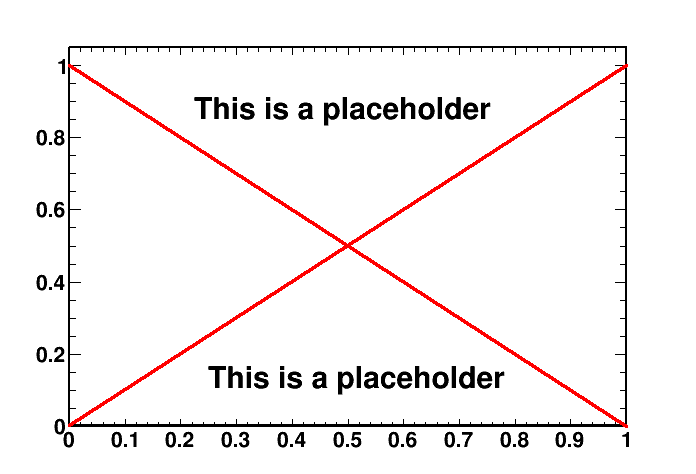
\includegraphics[width=.9\linewidth]{pic/dummy.png}
%  \caption{This is a dummy plot.}
%  \label{fig:dummy}
%\end{figure}
%
%\section{A section}
%\label{sec:section}
%Here we have Section \ref{sec:section}. \todo{This is a TODO marker} You might need this.

\section{Our Milky Way}

\subsection{General properties}


\begin{figure}[h]
  \centering
  \begin{minipage}[h]{0.45\textwidth}
  	\centering
	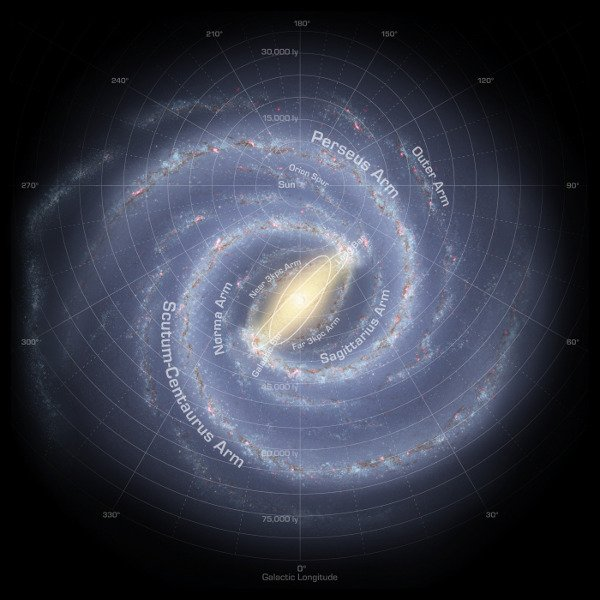
\includegraphics[width=1.\linewidth]{pic/theory/top_galaxy_map.jpg}
  	\subcaption{source: http://galaxymap.org/drupal/node/171}
  	\label{fig:top_gal_map}
  \end{minipage}
  \hfill
  \begin{minipage}[h]{0.45\textwidth}
	  \centering
	  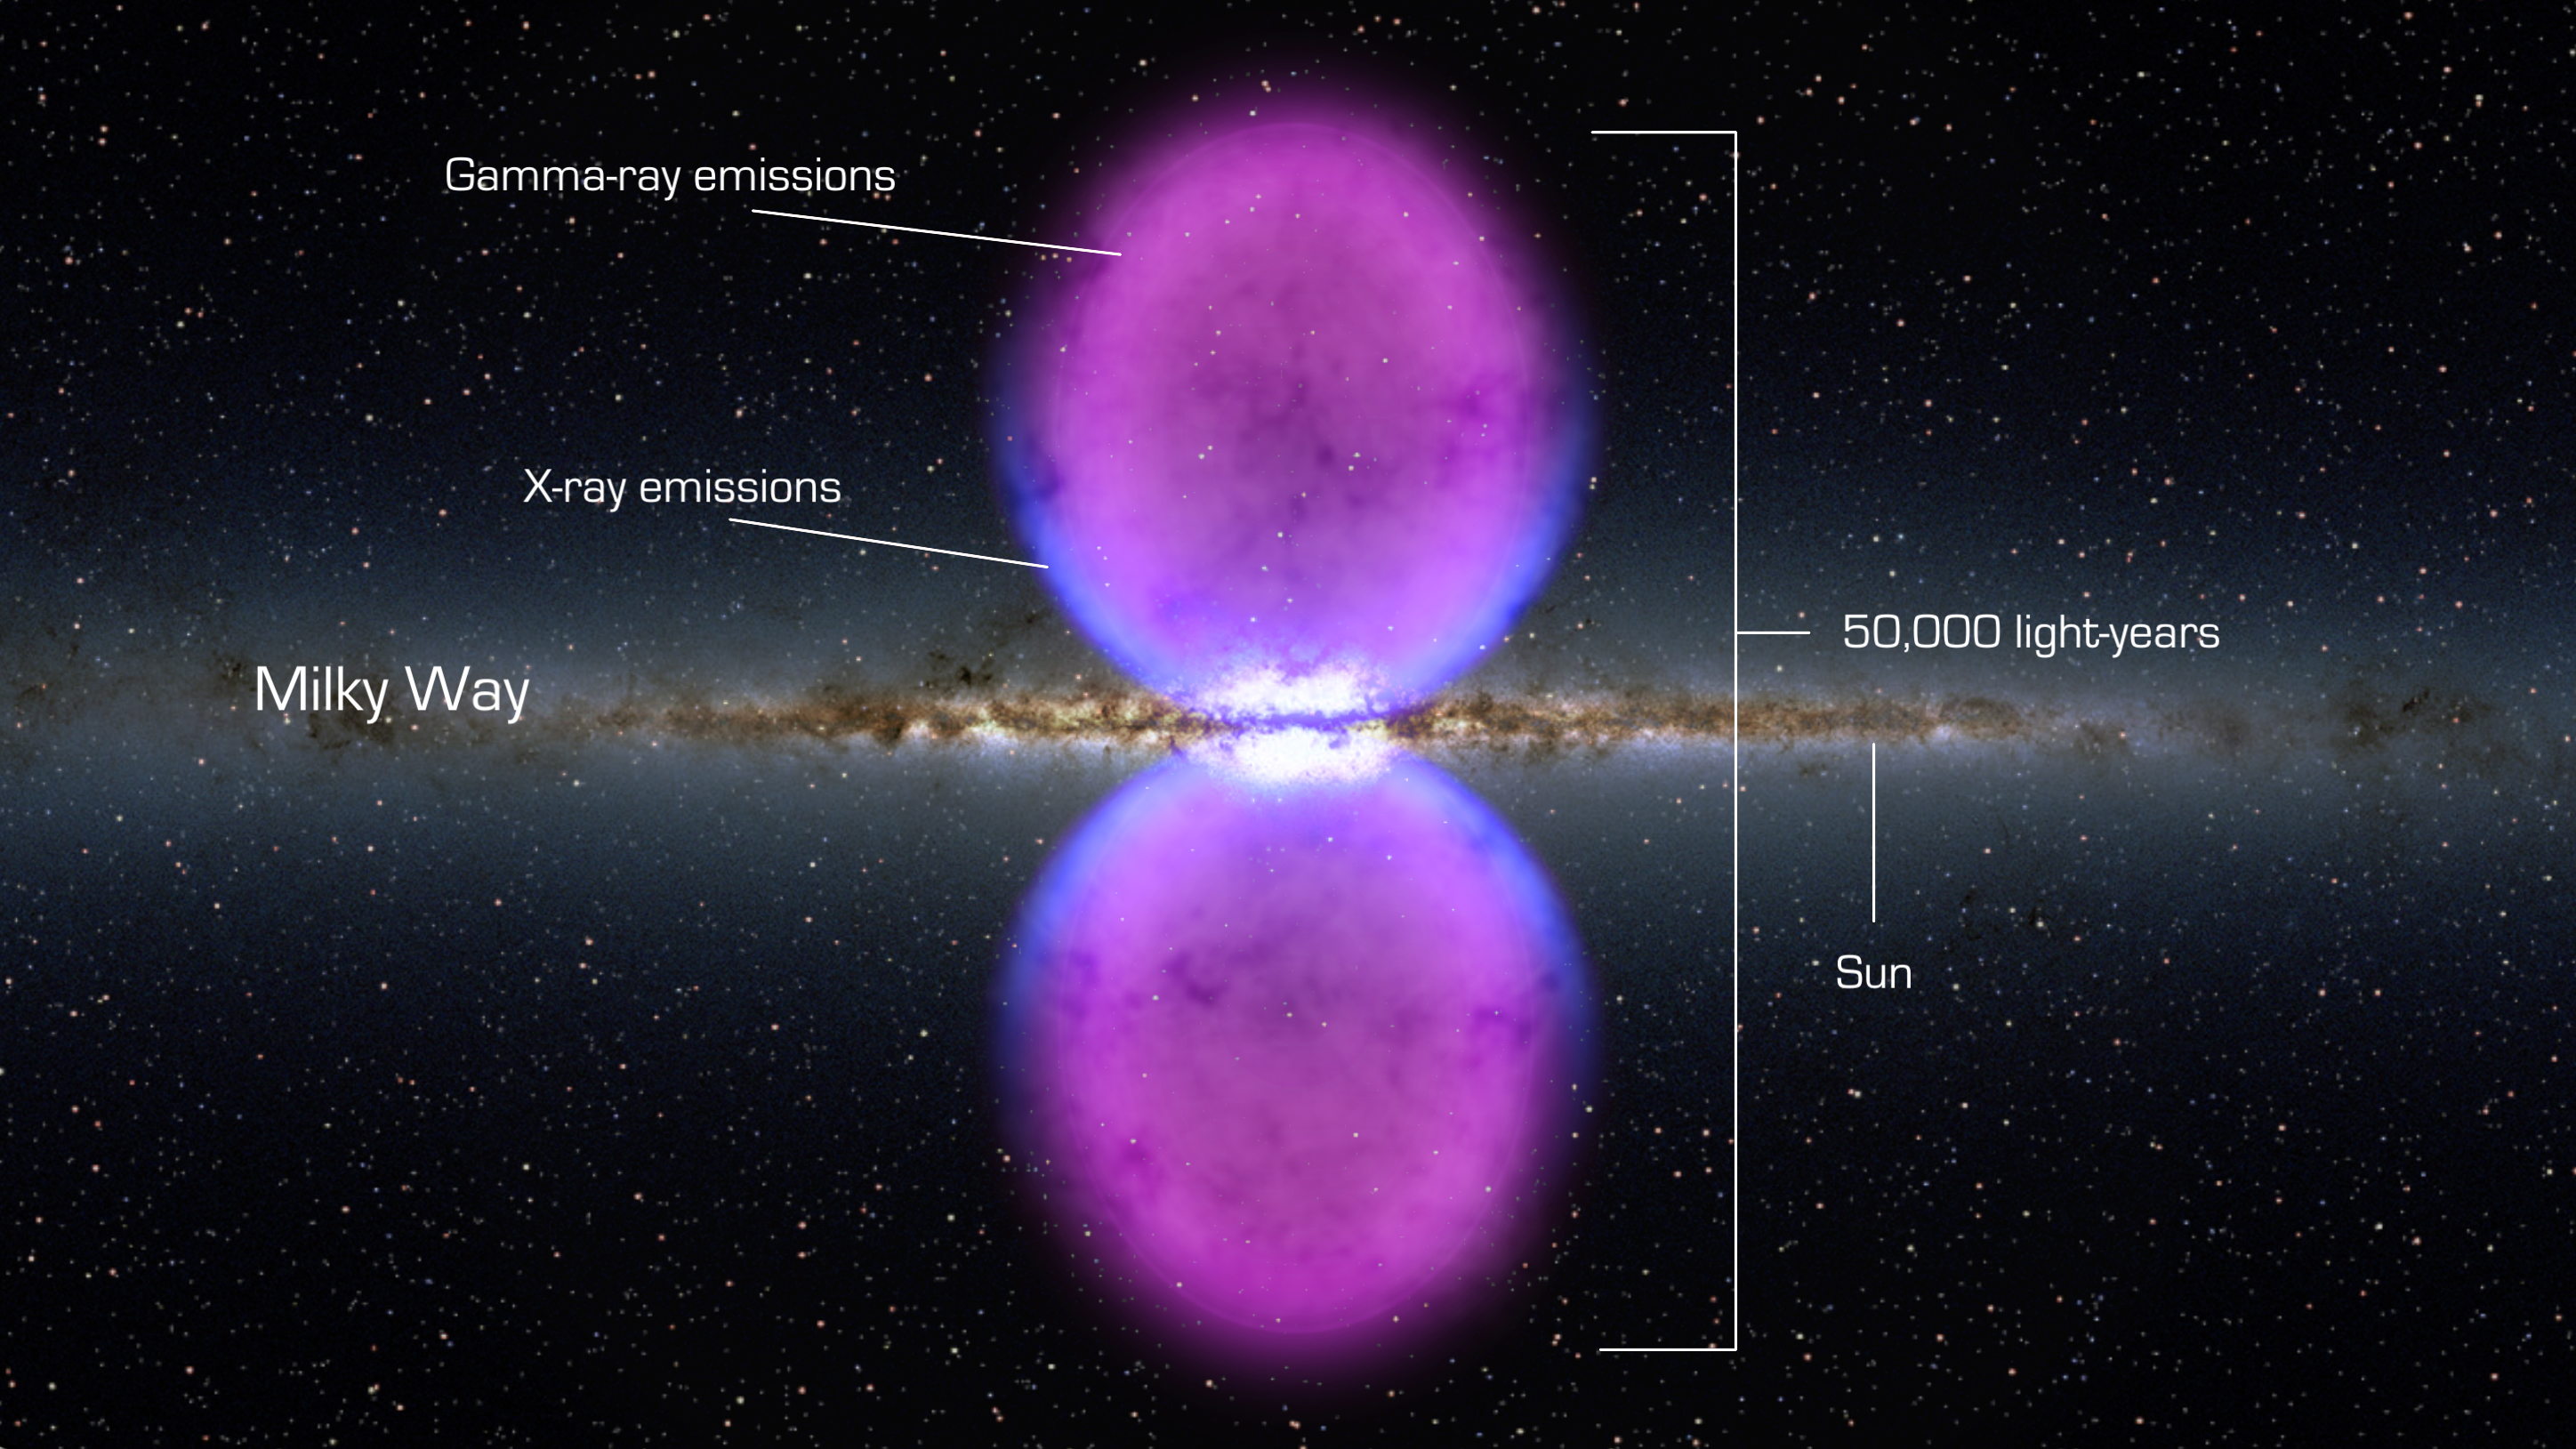
\includegraphics[width=1.\linewidth]{pic/theory/Fermi_bubble.jpg}
	  \subcaption{source: NASA's Goddard Space Flight Center}
	  \label{fig:fermi_bubbles}
  \end{minipage}
  \caption{The Milky Way, as seen from two different angles.}
  \label{fig:Galaxy_maps} 
\end{figure}

For a long time, people thought the universe was constituted of only one galaxy, the Milky Way, the one in which the Sun and the Earth orbit. The discoveries of other galaxies in the universe came only in the 20's thanks to Edwin Hubble. There is still a lot of unknown  around those objects, but the Milky way is pretty well known and will play a major role in the following chapters. Its shape, density and composition are three main factors playing a role in cosmic ray physics and can not be avoided.

First of all, the Milky Way is a barred spiral arm galaxy, meaning it has two main spiral arms, connected in their center by a straight galactic bar. Those arms and bar have higher matter concentration than the rest due to the way stars orbit around the center. Its diameter exceeds 40 kpc for a mass of around $10^{12} M_\odot$ and a thickness under 1 kpc. The Sun and the Earth are rotating 8 kpc from its center in 240 Myr.
All the different objects of the galaxy can be found in this thin disk of matter, mainly in the spiral arms. It includes the stars, planets and over massive objects, but also all the dust and gas clouds. As seen from the Earth, the disk looks like a narrow band of a few degrees in latitude, but with a very high concentration of gas and dust.
In 2010, two large scale structures were detected to the north and the south of the GC. With a diameter of 7kpc, these two "bubbles" extend up to 40 degrees in latitude and 20 in longitude. They are a source of high energy gamma-rays and were detected by the Fermi Large Area Telescope (LAT).

The disk of the Milky way is composed of matter in different forms, like stars, gas or dust. Stars are one of the first source of the interstellar radiation field (ISRF). They can be compared to black body radiating at different energies depending on their temperature. They are the main source of UV photons, that play a major role in the gas evolution. Stars are forming inside gas and dust clouds, collapsing on themselves under their own gravitational pressure.
The gas is composed in the vast majority of hydrogen, but heavier elements and even molecules can be found at the center of large clouds where ultra-violet light can not penetrate. One of these is the CO molecule, often used to as a tracer of molecular clouds. Even if molecules can only be found where the UV starlight can not break them apart, molecular clouds (MC) will designate large region of gas and dust, that can possibly contain stars inside.
\todo{add gas/dust ratio} Dust is also present in the galactic disk. It can be warmed by the starlight, and cooled via infrared light emission. This IR source is also part of the ISRF.

Electromagnetic field runs all across the milky way, taking its source in rotating stars, molecular clouds, or any moving charged particle. It has been observed and measured, but it is very complex and has no favourite direction at small scales (interstellar scale).

\subsection{Dark Matter}

\begin{figure}[h]
 \centering
 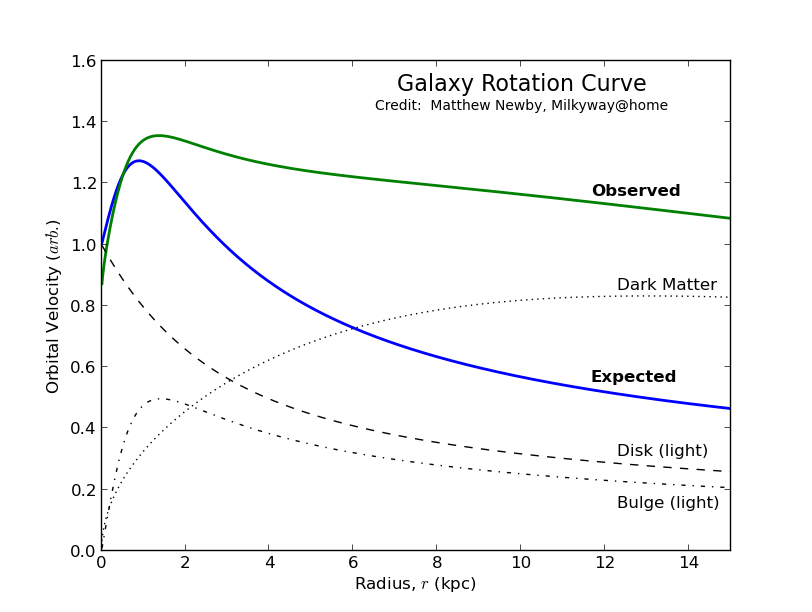
\includegraphics[width=.5\linewidth]{pic/theory/gal_rotation_curve.png}
 \caption{Orbital velocity of the Milky Way as a function of the radius. A clear discrepancy between the theory and the observation can be seen above a 2 kpc radius. Source: Matthew Newby, Milkyway@home}
 \label{fig:gal_rotation_curve}
\end{figure}


The shape of spiral galaxies is well known today, with thousands of examples throughout the universe. This knowledge can be used to mathematically simulate them, and in particular their rotation speed as a function of the distance to the center. It was a big surprise when the observed angular speed did not match the theory. One of the solution to explain this difference was the introduction in the standard model of dark matter (DM), which was suppose to bring a lot of invisible mass into the system. It still has not been observed and a few theories exist on its exact nature. But even without knowing exactly what it is, its mass distribution can still be deduced from the observed rotation curve of the galaxy. The predicted distribution is a spherical halo extending way beyond the 40 kpc of the galactic matter disk. It's density peaks in the GC, and decrease with the radius following a particular density profile. The exact profile is not known, but a popular one is the Navarro-Frenk-White (NFW) profile defined as follows :

\begin{equation}
\rho (r) \propto \frac{1}{\left( r/r_S \right) \left( 1 + r/r_S \right)^2 }
\end{equation}

where $r_S$ is the scale radius.

One of the most popular is the Weakly Interacting Massive Particles (WIMP). They are supposed to be non standard particles with a large mass, neutral, and only sensitive to the weak force, making them very difficult to observe. But no particles of the standard model has the right properties. 


\section{Tools}
%Energy spectra
%Intensity, Flux

To speak about cosmic-rays, one often speaks about their spectral shape, or energy spectrum. These terms refer to the particle flux ($\Phi$ in $GeV^-1.s^-1.cm^-2.sr^-1$) as a function of their energy (in $GeV$).  In other terms, how many particles of a given energy would a one centimeter square instrument observe in one second. This can often be modeled by a power law of the form $\Phi \propto E^{-\alpha}$  where $\alpha$ is called the spectral index. If $\alpha$ is small, the spectrum is said to be "hard", because there are an important proportion of high energetic particles. On the contrary, a "soft" spectrum has a bigger spectral index and describe a lower density of high energy particles compared to low energies.

In the following chapter though, the preferred representation of the energy distribution is via the energy flux (in $GeV.s^-1.m^-2.sr^-1$), simply obtained by multiplying the particle flux by its energy square ($E^2 \times \Phi(E)$). In other terms, how much energy does the instrument receive every second for particles of a given energy E. This is only done to facilitate the reading of the graphs and does not affect the underlying physics.

The terms of "soft" and "hard" can be applied to any kind of energy spectrum, even if it is not a power law, it will only describe the relative proportion of high and low energy particles.




\section{Physic of cosmic rays}

\subsection{Creation of CR}
\label{sec:creation_of_CRs}
%		-supernovae (SNR)
%		-AGN (activ galactic nuclei)
%		-pulsars, quasars

Several sources of cosmic rays exist in the universe. Cosmic rays are very energetic and thus can only be produced by very energetic phenomena. Particularly powerful events are supernovae, ejecting relativistic particles during the burst. The dying star will eject a lot of its mass to form a supernova remnant (SNR) surrounding either a white dwarf, a neutron star or a black hole depending on the initial mass of the star. These SNR could also play a role after the explosion via the Fermi process. An already energetic particle would bounce in the shock wave created by the explosion, and gain energy via hydrodynamic or magneto-hydrodynamic before escaping when the energy is sufficient.
An other important source of cosmic rays are the pulsars. These rapidly rotating neutron stars and their intense electromagnetic field create high energy particles such as protons and electrons. This can last as long as the pulsar rotates fast enough, but it can takes 10 to 100 Myrs before the turn-off occurs.
A third source are the actives galactic nuclei (AGN), also known as quasars. These objects consist of a super-massive black hole at the center of a galaxy. First discovered thanks to their radio emission, they are also able to eject CR, certainly via Fermi or centrifugal acceleration.


\subsection{Propagation of CR}
%Propagation through the galaxy
%	-random B field -> no way to backtrace a CR
%	-interaction, shocks in MC
%	-Diffusion coefficient
%		-Can be different in disk, bubbles, or outside
%	-different diffuse coef mean different densities
%		-in MC, bubbles, outside
%		-can observe this inhomogeiniies via gamma rays

Once they are emitted, the cosmic rays propagate through the galaxy under the influence of different interactions.
The first thing to consider is the very complex magnetic field created by all sorts of objects, from stars to molecular clouds or any distribution of charged particles. It is not particularly strong \todo{put values} compared to the heliosphere or what can be created on Earth, but its very large scale suffice to bend the CR's path in all direction until the point where it is impossible to backtrack their origin without exact knowledge of every detail of the galaxy.
An other possible interaction is the collisions with other particles. It will obviously depends on the density distribution of those colliders along the path of CRs. For example, we can expect a higher number of collision in the disk, where the density of molecular clouds is the highest.

All these influences can be modelled by a diffusion model, mainly defined by its diffusion coefficient D, which describes the average distance travelled by the particles during a certain time. The higher the coefficient, the faster a particle will diffuse in the galaxy. On the contrary if D is small, the particle's path will be bent in every direction so often that it might stay close from its source for a longer time. Each phenomenon can be attributed one of those coefficient to describe its effect on the cosmic rays, and adding them up gives the effective coefficient. \todo{give values for Dmag, Dcoll...}
While the diffusion coefficient for the galactic magnetic field can be taken as constant throughout the milky way, the diffusion coefficient due to collision is proportional to the particles density. We can then expect a smaller coefficient in molecular clouds, where the density can reach \todo{value!}.

This coefficient will also define the cosmic ray densities in various locations of the galaxy. Indeed, the more a particle's path is twisted and convoluted, the harder it will be to move away from its origin. This way, a higher density of cosmic rays can be found in low diffusion coefficient areas like molecular clouds. In comparison, the region outside the galactic disk has a low density of CR due to a weak electromagnetic field and small gas and dust density. 
However, the bubble region is outside the disk and has a higher concentration of high energy CR than other regions outside the disk. This is due to a direct outward emission of CR from the GC region. With a high diffusion coefficient, these CR are ejected light years away (see Fig. \ref{fig:fermi_bubbles}), forming two symmetric regions extending north and south up to 40 degrees in latitude.

The consequences of such diffusion processes is an isotropic cosmic-ray sky on Earth. In whatever direction the instruments look at, they measure the same CR flux. This complicate a lot their study, since no information about their origin or their journey can be learned from direct observation. 
%It is where gamma-rays enter the scene to play a major role in the indirect detection methods.

\subsection{Energy losses}

Travelling through the galaxy tedious, even for a high energetic particle if not more. In fact, every time a particle collides with another less energetic, or is deflected by a magnetic field, it looses energy. And depending on its energy and its surroundings, a particle will not always loose energy at the same rate.
If the particle has a particularly large energy, it will mainly encounter lower energy particles and will loose energy very fast. But if the particle is in a molecular clouds where all the others are around the same energy, every collision will only change its energy a little up or down, and it will basically stay the same.
This process is important to explain changes in CR spectral index. Indeed, the high energy particles emitted directly at the source, will loose energy faster than the less energetic ones, and then become itself a low energetic particle, populating the lower part of a spectrum. This way, a hard spectrum of a source can soften over time to resemble a propagated spectrum. The theoretical index values for a propagated spectrum is 3.85, against 2.1 for a source spectrum. \todo{cite}
This phenomenon can happen more or less quickly depending if the source emits in the disk where a lot of collision happen; or perpendicular to it, where the density of particle is not so high and the energy losses are more rare.



\subsection{CR as observed from Earth}

\begin{figure}[h]
 \centering
 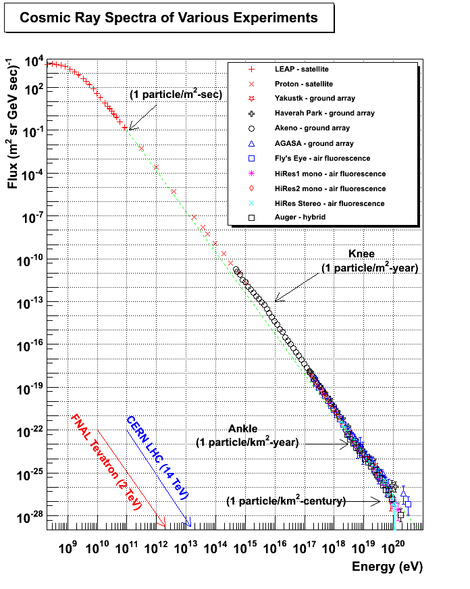
\includegraphics[width=.5\linewidth]{pic/theory/CR_spectrum.png}
 \caption{Cosmic ray spectrum as seen by several experiments. The "leg" can be seen with a "knee" around $5.10^{15} eV$ and two different spectral indices on both sides. Two of the best human attempts to recreat very high energetic particles are shown and give an idea how powerful CR can be.
 Source: http://www.physics.utah.edu/~whanlon/spectrum.html}
 \label{fig:CR_spectrum}
\end{figure}

The one and only CR spectrum that can be obtain from observations on Earth is shown on Figure \ref{fig:CR_spectrum}. It is the same in every direction as far as the measurement uncertainties can tell. The isotropic arrival direction of CR is measured with great care and any anisotropy, if existing, is below the instrument precision.
The CR spectrum is composed of three main features that form a "leg". The "knee" around $10^{7} GeV$ marks the separation between two different power laws in $E^{-\alpha}$. A slightly harder one below that is thought to be composed of galactic CRs, and a softer one above that is supposed to be of extra-galactic origin. The spectral index does not change much, from 2.7 below to 3 above, due to different production mechanism.
As indicated on Figure \ref{fig:CR_spectrum}, the corresponding flux of particle is very low and statistical fluctuations are not negligible at high energies. Especially at the "ankle", above $10^9 GeV$, where only very few particles were detected.


\subsection{Gamma-ray creation}
%		-pion decay
%		-bremmstrahlung
%		-inverse compton

Since the cosmic rays we observe on Earth can not give us a clue about their origin, some indirect detection methods are required. Luckily, cosmic rays interact in a lot of ways with their environment, as described in the previous section. These interactions can leave detectable traces that can be observed. The most common is the production of light, via creation of high energy photon in the GeV range. Once created, these gamma rays can be blocked or absorbed, but not deflected. Linking the gamma-ray and cosmic ray requires to know the processes in play. Here is a list of the main phenomena.

\subsubsection{Pion decay}
%Explain phenomenon
%Explain expected gamma ray spectrum, propagated proton distribution.

%The high energy protons can produce $\pi^{0}$ which decay almost immediately in 2 gammas of equal energy.

The hadronic cosmic rays  particles interact with the interstellar medium and can lead to pion $\pi^0$ production. Any CR nuclei can result in pion production, but since protons are the most abundant particles, they will dominate the production. 
These newly created pion can rapidly decay into a pair of gamma-rays (99\% of the time) or e+e- pair (negligible).




\subsubsection{Bremsstrahlung}
%Explain phenomenon
%Explain expected gamma ray spectrum


The charged CR passing near an other charged particle of the ISM or in a magnetic field will be deflected by the electromagnetic interaction. In the process, the CR will lose energy via the emission of photons. The energy of the latter will depend on the energy of the electron and the intensity of the electromagnetic field. The more the electron is deflected, the higher the energy of the emitted photons.
Even though proton CR are charged, the main source of bremsstrahlung gamma-rays is electrons and positrons. This is due to the much lower mass of the electrons, making them easier to deflect.

\todo{give numbers for B field and proton in MC}


\subsubsection{Inverse Compton}
%Explain phenomenon
%Explain expected gamma ray spectrum


A third process can take create gamma-rays when the CR electrons interact with a photon of the interstellar radiation field (ISRF). When a high energy electron collides with a low energy photon, the electron can transfer some of its kinetic energy to the photon, giving him enough energy to enter the gamma range.

So number of gamma rays coming from inverse Compton is directly linked to the electron distribution and the ISRF of the galaxy. The latter is composed of three major components, the starlight, the dust emission and the cosmological microwave background (CMB). The first component is directly linked to the star distribution, and will be dominant in the disk, where all the star are concentrated. The starlight emits as a black body, peaking in the UV range. The dust emission comes from the infra-red emission of warm dust. It will also be mainly present in the disk, since the dust clouds are pretty flat. Finally, the CMB is peaking in the microwave range but is uniformly present everywhere in the universe, and therefore in the galaxy. It will be dominant where the two others are negligible, namely outside the galactic disk.


\todo{talk about synchrotron and ionization losses}

\subsubsection{Other sources}
%Gamma-ray burst
%Pulsars

The three previously described processes are general processes that can happen everywhere at any energy. But even though the process might always be the same, two class of sources can be defined: the diffuse and the point sources. 
The first correspond to all the CR propagating through the ISM and interacting with its components. It will be the object of study of the following chapters. 
The second are the gamma-rays produced directly at the CR origin (in SNR, AGN or pulsars as described in section \ref{sec:creation_of_CRs}). Every one of these event should be studied separately and are still not understood perfectly. Since these sources are very far away and can not be resolved by the instruments, they will be referred to as point sources in the following chapters. The spectral shape of these events is generally known and categorized as a function of the event type. This makes the recognition easier and both emissions can be separated 
this way.


%Other sources of gamma-rays exist in the universe that will complicate the observations. Gamma-rays are very energetic and thus can only be produced by very energetic phenomena. The gamma-ray bursts for example were discovered in the late 60's when U.S. satellites were build to detect nuclear weapon tests. These two events produce gamma-rays, but the first one is much more powerful, sometimes emitting more energy than the Sun will in its entire life-time. It is thought to be emitted by supernovae in distant galaxies or the merging of two neutron stars. These events are short (from milliseconds to hours) and will not be dominating the observations.
%An other source is the pulsar gamma-ray emission, and even though they are less energetic, their long-term production make them one of the first sources of observed gamma-rays. It can be said the same about quasars or active galactic nuclei (AGN).
%All these sources produce high energetic cosmic-rays that will lose energy via the different processes described earlier, and produce gamma-rays. 


\subsection{Gamma-ray observations}

Gamma-rays are not easy to observe from Earth, simply because they are absorbed by the atmosphere. It is a chance for life to develop, but complicates their observation. To measure them, the instrument has to be launched in orbit above the atmosphere, where gamma-rays are not yet absorbed. For example the Fermi Large Area Telescope (LAT) mounted on the ISS do the job with a lot of success. This instrument maps the gamma ray sky between 20 MeV and 300 GeV \todo{cite}, detecting all the point sources emission, but also the diffuse background emission.


%The diffuse cosmic ray emission that we are interested in can be obtained after modeling and subtracting the contribution of the over sources. This allows us to compare the observation with the models we obtain from the previous three interactions.


In theory, the knowledge of the processes that generate gamma-rays from cosmic-rays and the precise composition of the Milky Way should allow to explain the observations. Propagation models and simulations are able to output the expected energy spectrum of gamma-rays reaching Earth from an initial distribution of cosmic-rays (not taking the point sources into account). But some problems show up when confronting the theory and the observations, as will be discussed in the following section.



\section{What are the unresolved problems of the precedent chapter}
%What are the unresolved problems of the precedent sections:
%	-Bad fits in bubbles and disk	
%	-Spherical gamma-ray excess in GC when fitting spatial templates
%		-DM studies
%			-Hooper
%			-others...
%		-MSP studies
%			-Fermi
%			-Hooper
%			-Weniger
%	-High energy tail flux too hard
%	
%
\begin{figure}
 \centering
 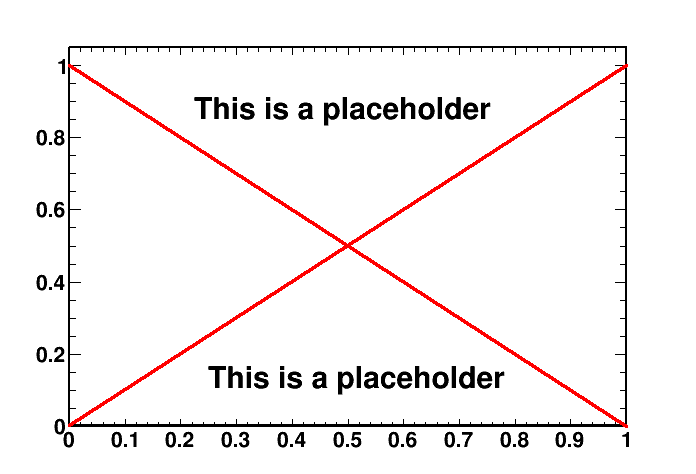
\includegraphics[width=.9\linewidth]{pic/dummy.png}
 \caption{chi2 distribution of first fits (not mines)}
 \label{fig:first_BKGonly_fits}
\end{figure}



\begin{figure}
 \centering
 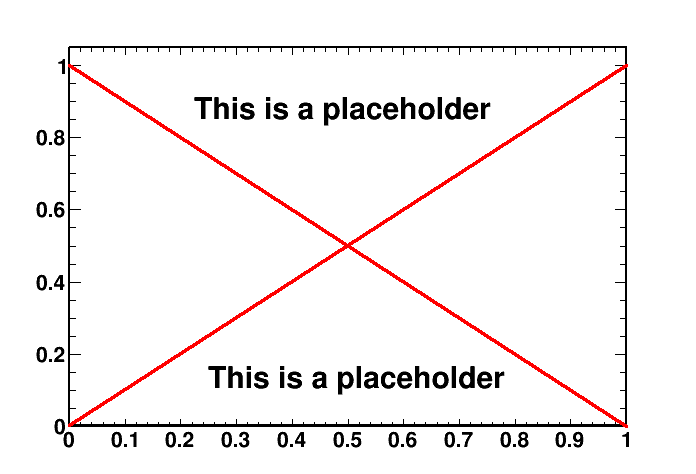
\includegraphics[width=.9\linewidth]{pic/dummy.png}
 \caption{shape of the excess}
 \label{fig:first_BKGonly_fits}
\end{figure}

Several studies have already tried to see how the predictions of the gamma rays emission and the observations compare. The three main phenomena were modelled to try to recreate the spectrum observed here on Earth. The results are clear, they do not always match.
Even though the observations of the poles or any high latitude regions can be well explained by a PCR, BR and IC component, the models have troubles to reproduce the surroundings of the galactic disk, and in particular the GC or the Bubbles. 
Two main problems can be identified. A high energy deficit in the models, where the high energy tail (> 50 GeV) observed can not be reproduced, and a spherical excess centred in the GC around 2 GeV.

The first one shows a lack of high energy cosmic-rays in the models. A mean of injecting more relativistic particles has to be found in order to fill this gap. One explanation could be that we do not observe only diffuse emission in the disk. The point source emission could not be totally subtracted due to the high density of sources. The CR that do not have the time to propagates have a harder spectrum, thus providing a higher ratio of high energy gamma-rays.

Two main ideas have emerged to explain the spherical excess.
First is the presence of dark matter in the galaxy in the form of weakly interacting massive particles (WIMP). The spatial distribution of these particles would follow a Navarro-Frank-White (NFW) profile centred at the GC. They are also expected to produce gamma rays when annihilating with each other via hadrons production. In theory, if the mass of a WIMP particle is around 50 GeV, the expected gamma spectrum would peak around 2 GeV, where the excess is observed. \todo{cite}
The study of the excess could put strong limits on the mass and annihilation cross section of such WIMP and confirm, or infirm the theory.
The second theory does not involve new physic, but unobserved millisecond pulsars. They would also be spherically distributed around the GC and their gamma spectrum peaks around 2 GeV. A few thousands of them would be needed to recreate the intensity of the excess. The main default of this explanation resides in the fact that we have observed only a few hundreds pulsars so far when we expect ten times more.








































%% ================================================================================
\chapter{Method}
\label{ch:method}
%% ================================================================================

\section{Data origin}
\label{sec:Data_origin}
%	-Data origin
%		-Fermi collaboration
%		-LAT
%		-Fermi FTOOLS
%		-point source subtraction
%		-pass7 vs pass8
%			-wider energy range
%			-better statistical and systematic errors
%			-better event selection




%(Maybe also some spectrum with pass7 and pass8 to see the differences.)

%\begin{figure}
% \centering
% 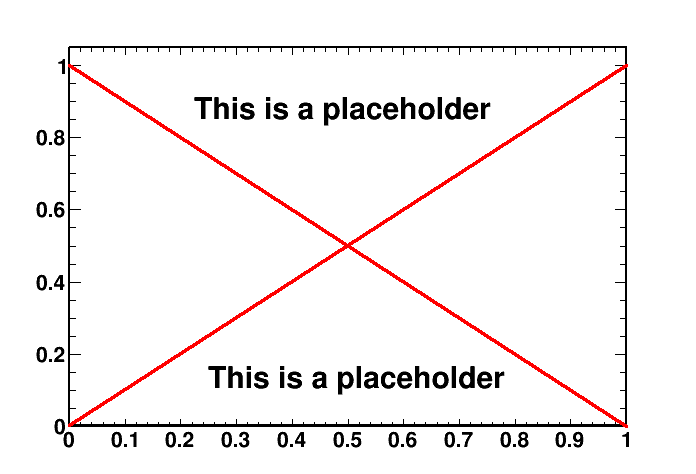
\includegraphics[width=.9\linewidth]{pic/dummy.png}
% \caption{Images of the exposure map}
% \label{fig:proton_spec}
%\end{figure}

\begin{figure}[h]
  \centering
  \begin{minipage}[h]{0.45\textwidth}
  	\centering
	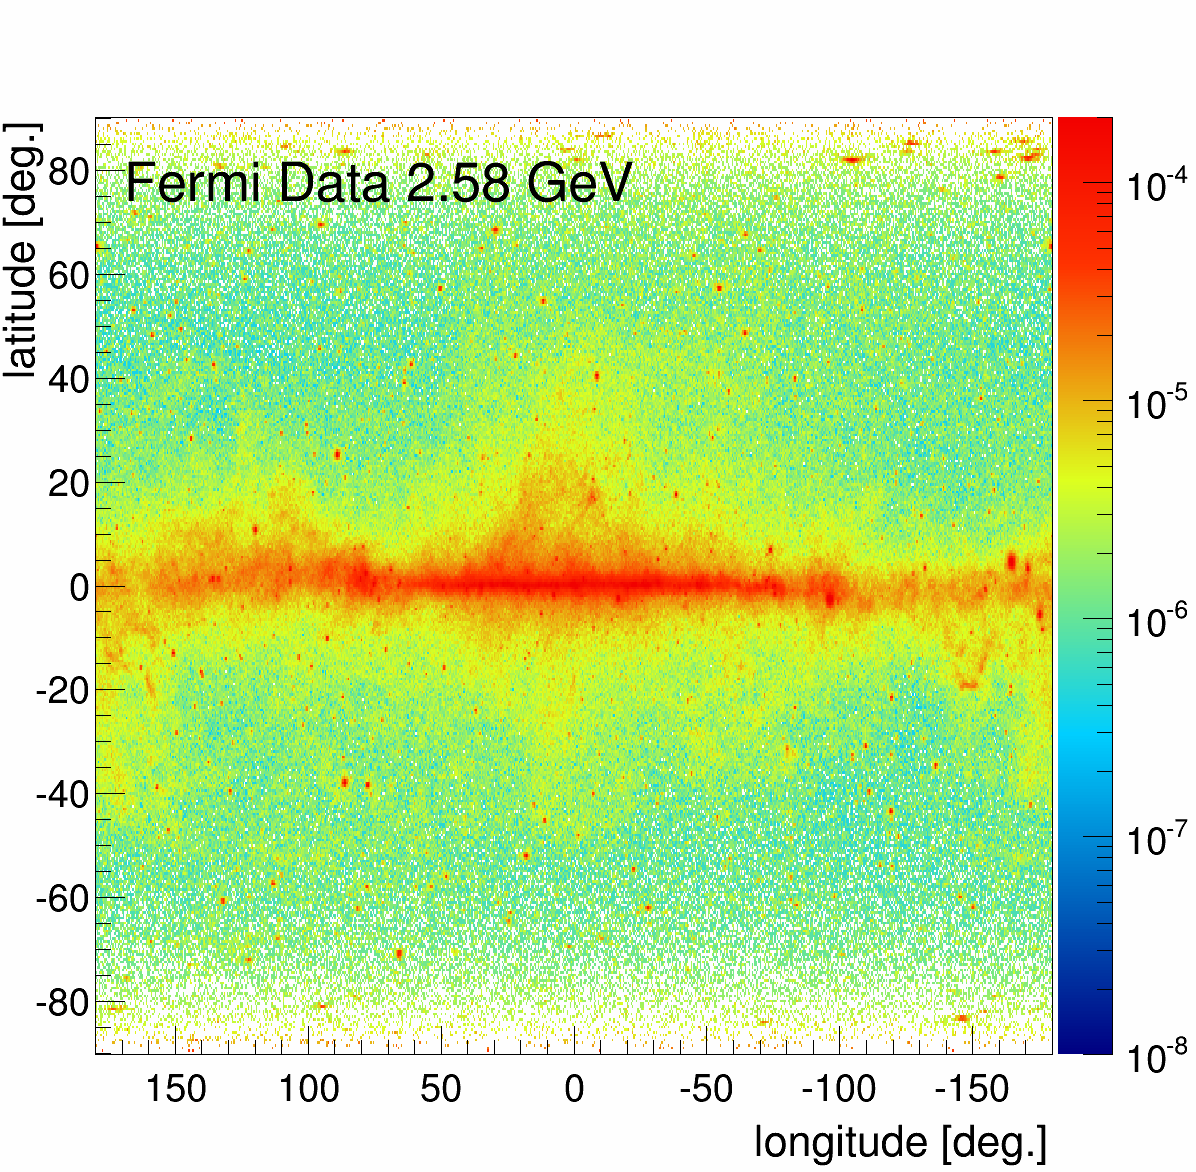
\includegraphics[width=1.\linewidth]{pic/method/Flux_FermiData_raw_E12.png}
  	\subcaption{}
  	\label{fig:raw_data}
  \end{minipage}
  \hfill
  \begin{minipage}[h]{0.45\textwidth}
	  \centering
	  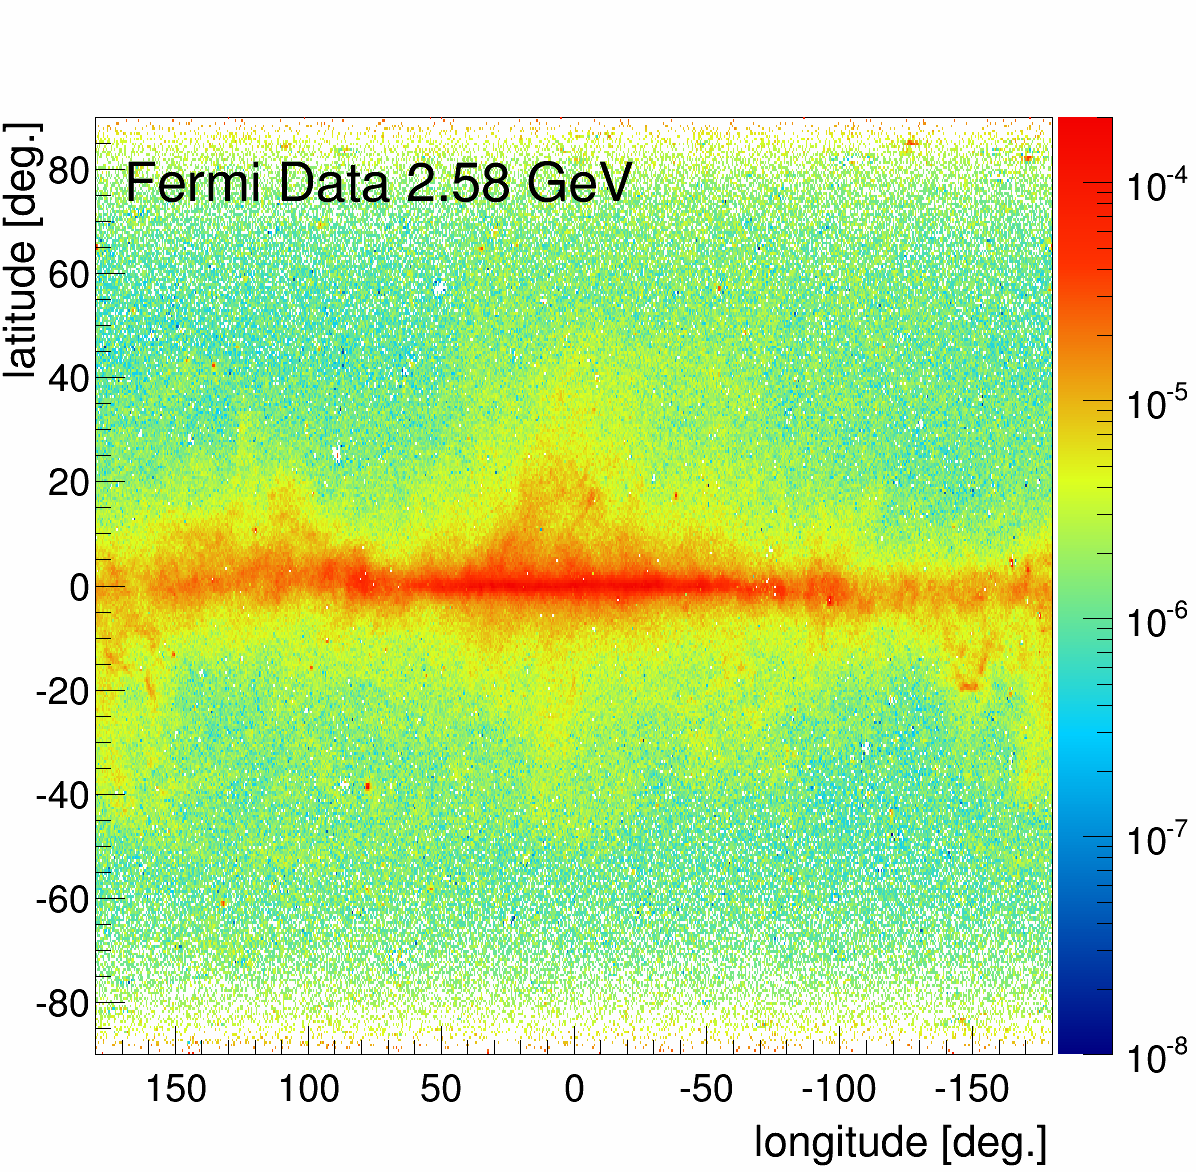
\includegraphics[width=1.\linewidth]{pic/method/Flux_FermiData-3FGL_E12.png}
	  \subcaption{}
	  \label{fig:data_ptsrc_subtracted}
  \end{minipage}
  \caption{Map of the gamma ray sky as seen by the Fermi telescope around 2 GeV. Measured gamma ray flux before (left) and after (right) point source subtraction in $GeV/s/m^2/sr$. Most of the spots formed by point sources have disappeared, leaving only the diffuse background emission from CR. The subtraction does not remove all point sources, and can create artificial "holes" in the map (for example at coordinates (90, 25) or (50, 60)). These can be disregarded as relevant data, or can also disappear when using a larger binning.}
  \label{fig:method_pass8} 
\end{figure}

All the following work is based on the measurement of gamma rays coming from intra- and extra-galactic sources. The quality and accuracy of the data is one of the most important points that will determine the general quality of the results. Thus it is capital to be certain that the gathering and treatment were done properly.

The Fermi Large Area Telescope (LAT) observes the gamma-ray sky since 2008 and provides all the data of this work. \todo{cite}
All the information and data are available on the web and anybody can access them, using the tools given by Fermi. \todo{cite}

The reconstruction method and data set of Fermi LAT is improved regularly, improving the statistics, the systematic errors and the point source subtraction. The latest data set to date, called Pass 8, is used for this work.
One of the most important steps in the treatment process is the selection of the events. Every photon measured is saved along with all its properties in a data file. Then this list is filtered to keep only the relevant observations. The filter can be based on the incoming direction, the energy or the time of observation, but also on the quality of the event reconstruction. This last cut can be critical. It will determine the chances that the measured event is in fact a gamma ray, and not some background noise polluting the data. The more strict the filter is, the less events are kept for analysis and the statistical errors increase. This work uses the CLEAN class recommended by the Fermi team for diffuse emission analysis. \todo{cite Fermi sciencetools}

The main parameters of the selection can be found in Tab \ref{tab:fermi_selection_parameters}.

\begin{center}
\begin{table}[h]
\centering
\begin{tabular}{|c|c|p{6.5cm}|}
\hline
\multicolumn{1}{|c|}{\textbf{Parameter name}} & \textbf{Parameter value} & \multicolumn{1}{c|}{\textbf{Description}}                                                                   \\ \hline
Event class                         & 256 (CLEAN)              & Quality parameter. Varies the level of background noise.                                                    \\ \hline
Event type                          & 3                        & Back+front event.                                                                                           \\ \hline
Time boundaries                     & INDEF                    & Selecting all events since beginning of observation.                                                        \\ \hline
Minimum energy (MeV)                & 58.4731                  & Minimum energy of the event.                                                                                \\ \hline
Maximum energy (MeV)                & 513056                   & Maximum energy of the event.                                                                                \\ \hline
zmax (degrees)                      & 90                       & Maximum zenith angle to get rid of the Earth contaminations, as recommended by the LAT instrument team. \\ \hline
\end{tabular}
\caption{List of the main parameters used for data selection. The exact script can be found in the appendix.}
\label{tab:fermi_selection_parameters}
\end{table}
\end{center}
\todo{add code in appendix and ref}


Another important point is the creation of the exposure map. It tells how long the telescope spent observing a given part of the sky. After dividing the count map by the exposure, a flux map is obtained that does not depends on the observation time of particular regions. For example, if the telescope observed the galactic center ten times more often than the Orion nebula , there is no way to know at first if the higher counts in the GC is due to the longer exposition time or a higher flux from this region.
%It is used to correct an observation bias. 

The goal of this work is to study the diffuse sources of gamma-rays from inside and outside the Milky Way. Of course, the LAT does not differentiate them from point source gamma-rays. This has to be done manually as the last step in the treatment process. A catalog of gamma ray point sources (3FGL) is available on-line on NASA website \todo{cite site}. This catalog lists most of the known and identified point sources, along with their spectral shape and flux. This information can then be used to model the number of counts coming from point sources and their spatial and energetic distribution. To achieve this, the point sources properties must be combined with the instrument properties. The point source flux is multiplied by the LAT exposure time corresponding to its position. This flux must also pass through the instrument and its defaults will deform the initial shape of the source. For a point source, the final image obtained by the detector is the Point Spread Function (PSF) of the telescope and is given with the Fermi tools. Every point source is convoluted by the PSF corresponding to the initial event selection, creating the final point source map as would be observed by the instrument.
Once this model map is obtained, it is subtracted from the data to only keep the diffuse emission (see Fig. \ref{fig:method_pass8}). Since the models are never perfect and all point sources are not listed, errors or anomalies in the observations can appear. Keeping the dataset up-to-date allows to use the latest catalogs and best reconstruction.


Once all the data treatment is done, a flux map of the entire sky in $counts/s/m^2/GeV/sr$ is produced. The map is divided in bins of $0.5 \times 0.5$ degrees on a Cartesian projection, also called cones. Every bin contains 30 logarithmic energy bins ranging from 60 MeV to 513 GeV with a 1.2 multiplicative step. Thus the final data cube is of dimension $720 \times 360 \times 30$. For visibility purposes, every energy bin is multiplied by its energy squared, becoming an energy flux in $GeV/s/m^2/sr$. This will be the default units used for the rest of this work.

The errors on the data are coming from two sources. First are systematic errors introduced by the instrument or the treatment process. They are around 3\%, but can increase for low or high energies (Fig. \ref{fig:LAT_sys_err}). These errors have multiple causes, mainly the PSF and the energy resolution (or energy dispersion) of the instrument. The plot shows how the systematic errors vary when correcting, or not, for these effects. The treatment shown in appendix accounts for energy dispersion.
The second source is the statistical errors, proportional to the square root of counts. This property will make them decrease when the acquisition time will increase. They are dominant at high energy (above 50 GeV) where fewer events are observed. On contrary at low energies (around 100 MeV), the systematic errors dominate. The final equation is the following :

\begin{equation}
\sigma_{tot} =\sqrt{\sigma_{sys}^2 + \sigma_{stat}^2} = \sqrt{\sigma_{sys}^2 + \frac{1}{N}}
\end{equation}


\begin{figure}[h]
 \centering
 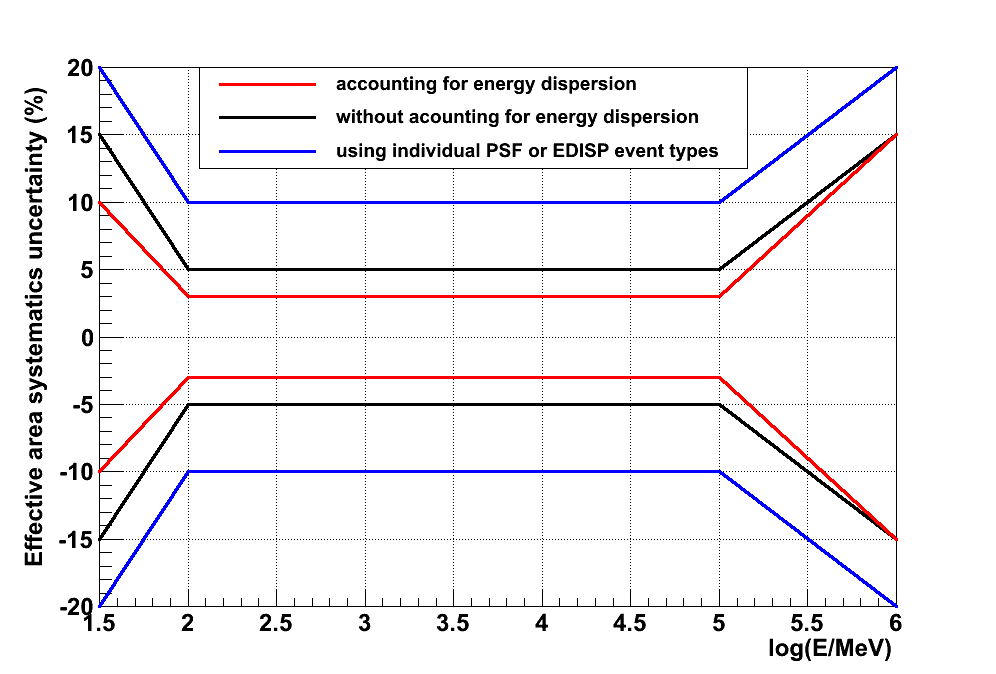
\includegraphics[width=.6\linewidth]{pic/method/LAT_sys_error.png}
 \caption{Systematic error for Pass 8 data as a function of the energy and the treatment procedure. The energy dispersion is the energy resolution of the instrument; this effect is known and can be corrected (in red), lowering the systematic errors. This is what was done for this study. The black line does not account for energy dispersion. The blue line shows the systematics for specific event types, and is used only for specific that can be ignored. The few percent gained with the energy dispersion treatment at very low energies (below a few hundred MeV), where the statistical uncertainties are not dominant any more, can be critical.}
 \label{fig:LAT_sys_err}
\end{figure}




\newpage
\section{Model components}
\subsection{From CRs to gamma-rays}
%Add subsection on how the gamma spectra are calculated. Don't forgt to explain how the 3 IC comps are managed}

The gamma-ray spectra used in this study are directly calculated from the CR spectra. The next section describes the CR distribution used to get the gamma-ray spectra corresponding to the modeled processes. Once the CR spectrum is defined, a propagation software \todo{cite}, DRAGON, is used to determine the emitted gamma-ray spectrum. For most of the components, the spectral shape does not vary depending on the direction, only its normalization does, but that does not play a role in the fitting method (cf \todo{section on fitting method}).
DRAGON uses a model of the galaxy (ISRF, matter distribution, etc...) and the input CR spectra for protons and electrons to produce gamma-ray spectra as an output for pion decay, bremsstrahlung and inverse compton scattering.


\subsection{Basic components}
%	-3 Basic components
%		-PCR
%			-proton CR follow power-law E^-2.849
%			?-try with break at 5-10GeV with index ~ -2.7 ?
%		-IC and BR
%			-electron CR spectrum E^-3.21
%			-break at 1GeV, index E^-3.21 + 2.4 below break

\begin{figure}[h]
  \centering
  \begin{minipage}[h]{0.45\textwidth}
  	\centering
	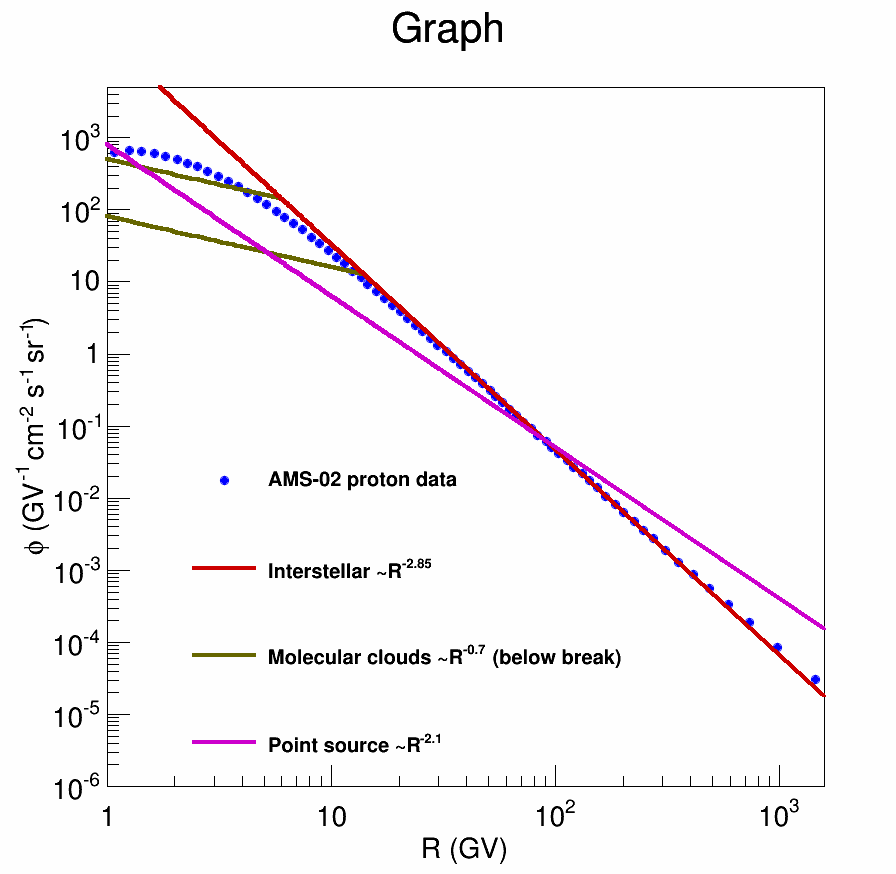
\includegraphics[width=1.\linewidth]{pic/method/./CR_protons_spectra.png}
  	\subcaption{}
 	\label{fig:proton_spec}
  \end{minipage}
  \hfill
  \begin{minipage}[h]{0.45\textwidth}
	  \centering
	  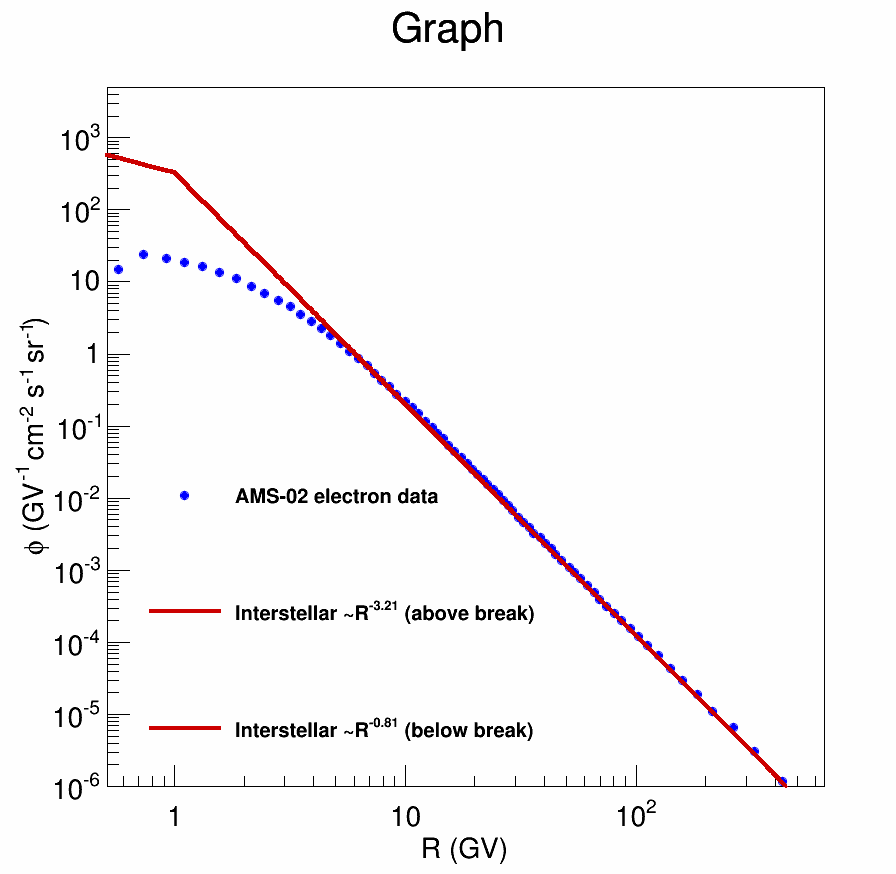
\includegraphics[width=1.\linewidth]{pic/method/./CR_electrons_spectra.png}
	  \subcaption{}
	  \label{fig:electron_spec}
  \end{minipage}
  \caption{Cosmic Ray spectra used to determine the gamma-ray templates. (a) Power-law proton spectra used to produce the proton based templates. In comparison, the measured data by AMS-02. The MC spectrum breaks are varying between the two shown here. Above the break, the index is the same than or propagated CR. (b) Power-law electron spectrum used to produce the IC and BR templates, compared once again with AMS-02 data. This time a break is introduced at 0.2 GeV.}
  \label{fig:cosmic_ray_spec}
\end{figure}


\subsubsection{$\pi^0$ production by propagated cosmic rays (PCR)}

%%% ARTICLE
The initial propagated proton spectrum for the PCR template is obtained from the observed proton data from AMS-02 \todo{cite[55]}. A good approximation is an unbroken power law ($R-\alpha$) with a spectral index ($\alpha$) of 2.85 at rigidities above 45 GV. At lower rigidities, the flux is not described by the power law because of solar modulations \todo{cite[56]}, as seen in Fig. \ref{fig:proton_spec}. %To find the best parametrization, several indexes and breaks were tested. The optimal parametrization was found by interpolation between the fits with the best test statistic. Finally, the gamma-ray data are well described by an unbroken power law for the protons with a spectral index ($\alpha$) of 2.85 at all rigidities.\\
%%% ARTICLE

%There is also the possibility to introduce a break around a few GeV, to have a slightly harder spectrum at lower energies.\\


\subsubsection{Inverse Compton (IC) and bremsstrahlung (BR)}

\begin{figure}[h]
  \centering
  \begin{minipage}[h]{0.45\textwidth}
  	\centering
	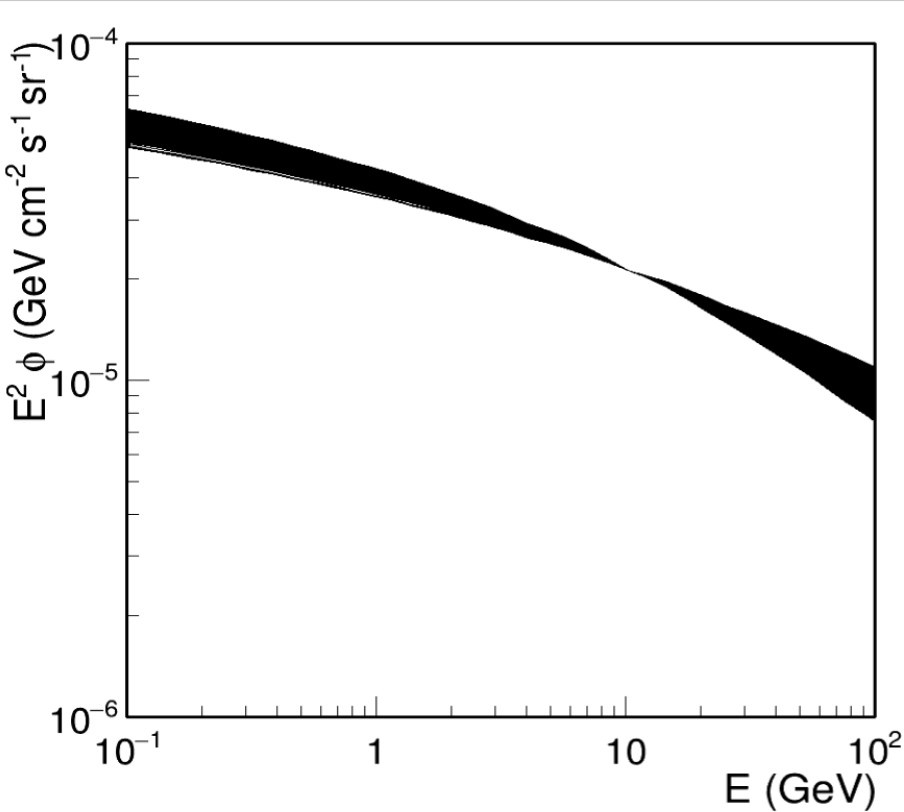
\includegraphics[trim={0 0cm 0 0.2cm}, clip, width=1.\linewidth]{pic/method/IC_variations.png}
 	\subcaption{}
 	\label{fig:IC_variations}
  \end{minipage}
  \hfill
  \begin{minipage}[h]{0.45\textwidth}
	  \centering
	  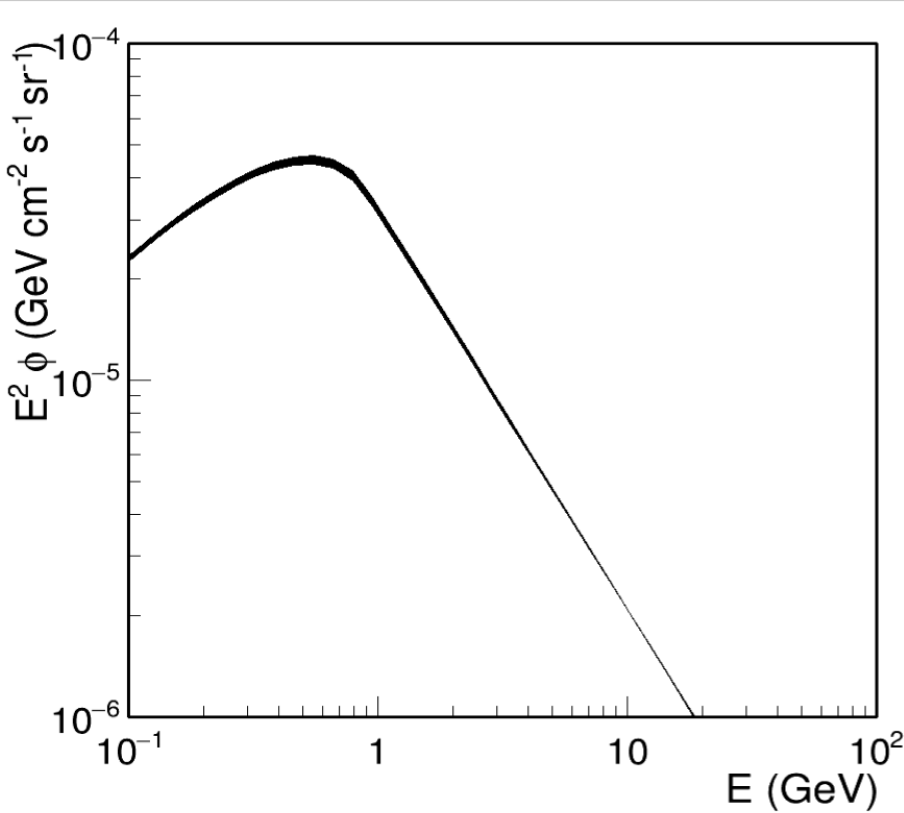
\includegraphics[trim={0 0cm 0 0.2cm}, clip, width=1.\linewidth]{pic/method/BR_variations.png}
	  \subcaption{}
	  \label{fig:BR_variations}
  \end{minipage}
  \caption{(a): Superposition of the inverse compton scattering template in every sky direction, normalized arbitrarily at 10 GeV. (b): Superposition of the bremsstrahlung template in every sky direction, normalized at 10 GeV. The CR electron spectrum use here has a break at 1 GeV, but its position does not influence the spatial variations. The variations of BR are very small and can be neglected.}
  \label{fig:IC_BR_variations} 
\end{figure}


The interstellar electron spectra need a break around 0.2 GeV with a spectral index of 3.21 above. This is compatible with the locally observed electron spectrum (see Fig. \ref{fig:electron_spec}). Below the break the optimal spectral index is 0.81, which implies a suppression of electrons. %The break point might be related to the fact that around 0.2 GeV electrons have the smallest energy losses, since above this energy synchrotron, BR and IC dominate the energy losses, while below this energy ionization losses become strong, thus depleting the electron spectrum below 1 GeV. A similar break in the electron spectrum was needed in the Fermi diffuse model \todo{cite[46]}.\\
The targets for the production of gamma-rays are the interstellar gas for BR and the interstellar radiation field (IRF) for IC, which are both strongly dependent of position%The latter consists of photons from the cosmic microwave background, the infrared radiation from hot matter, like dust and the star light
, so the photon composition varies with sky direction.
For this reason, the IC and BR templates are calculated for each sky direction. The variation over the sky is about $\pm 10\%$, as shown in \ref{fig:IC_variations}. 
The BR template only depends on the interstellar gas distribution, decreasing the variations considerably compared to IC, as shown in \ref{fig:BR_variations}.
%Note that the intensity of photons in the interstellar radiation field nor the gas density play any role in a template analysis, since the intensity of each contribution to the gamma-ray sky is determined by the fitted normalization factors in Eq. 1.



%The IC and BR spectra are both obtained from the interstallar electron distribution, taken here as a broken powerlaw with a break \todo{at 1GeV}. The index is 3.21 over the break and 0.8 below.
%The IRF is composed in the mostly by starlight (UV), and in with smaller contribution dust emission (IR) and the cosmic microwave background. The first two components of the IRF are position dependant, and this is why we have to calculate the IC spectrum for every sky direction.
%The BR component is directly linked to the gas, and charged particles distribution. This is also a reason too calculate the BR component in every sky directions. The variations are not too large.




\subsection{Additional components}
%	-2 or more additional components:
%		-SCR
%			-proton CR follow power-law E^-2.1
%		-MCR
%			-proton CR follow power-law E^-2.849
%			-break between 6 and 14GeV, index E^-2.849 + 2.149 below break
%		-DM
%			-Dark Susy
%			-Determination of Mass using best fit in CMZ
%		-MBR
%			-electron CR spectrum E^-3.21
%			-break between 6 and 14 GeV, index E^-3.21 + 2.4 below break
%	-Isosky
%		-Calculated from fermi model and adjusted in our fit

\begin{figure}[h]
  \centering
  \begin{minipage}[h]{0.45\textwidth}
  	\centering
	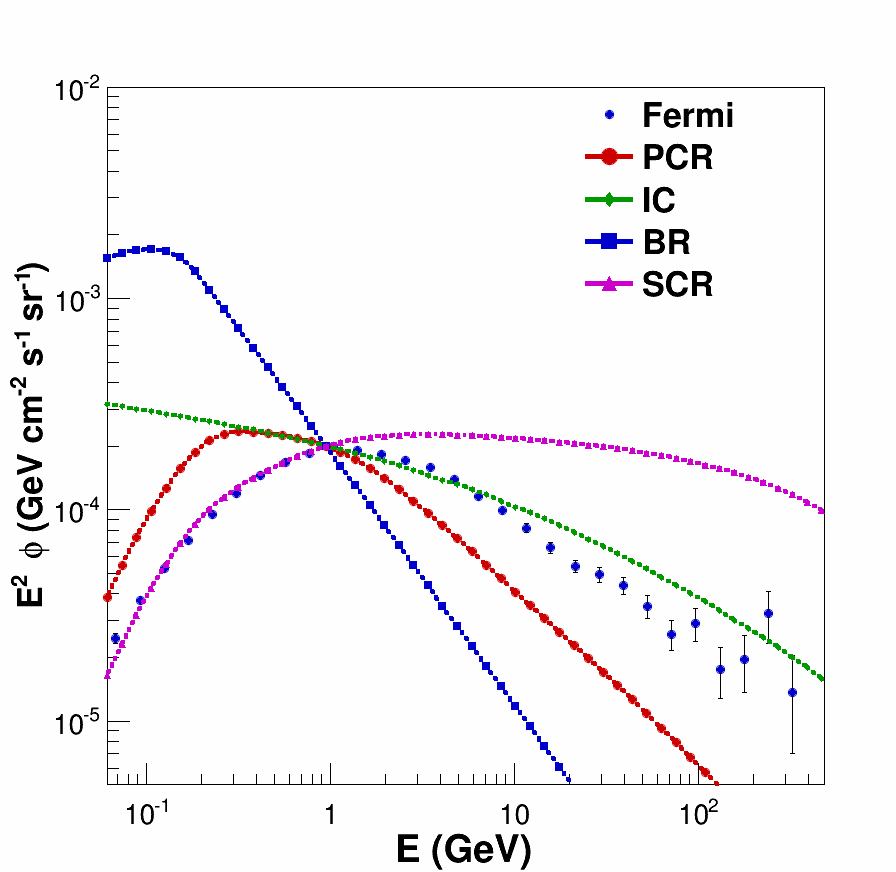
\includegraphics[width=1\linewidth]{pic/method/norm_bkg_comp.png}
  	\subcaption{}
 	\label{fig:norm_bkg_component}
  \end{minipage}
  \hfill
  \begin{minipage}[h]{0.45\textwidth}
	  \centering
	  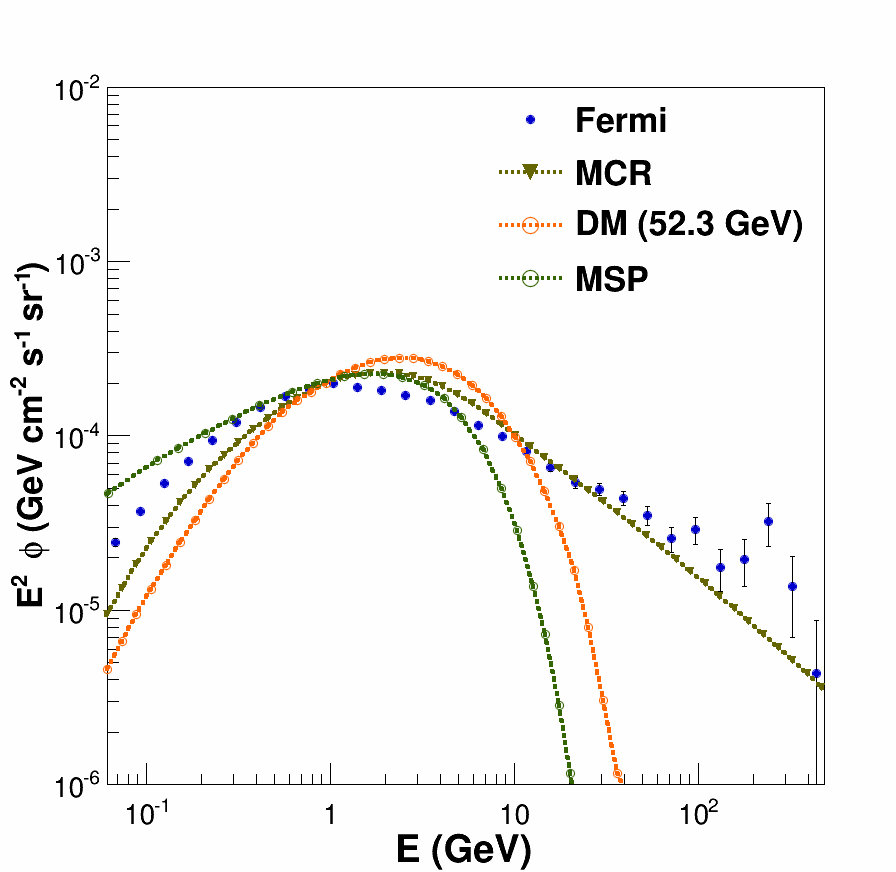
\includegraphics[width=1\linewidth]{pic/method/norm_excess_comp.png}
 	  \subcaption{}
 	  \label{fig:norm_excess_component}
  \end{minipage}
  \caption{(a) Comparison of PCR, IC, BR and SCR templates, normalized at 1 GeV. Measured data from the central molecular zone is shown as well. All four components have very different spectrum and index that make them easily identifiable by the fit. (b) Comparison of the three excess components, along with the data from the CMZ.}
  \label{fig:norm_spectra} 
\end{figure}




%
%\begin{figure}
% \centering
% 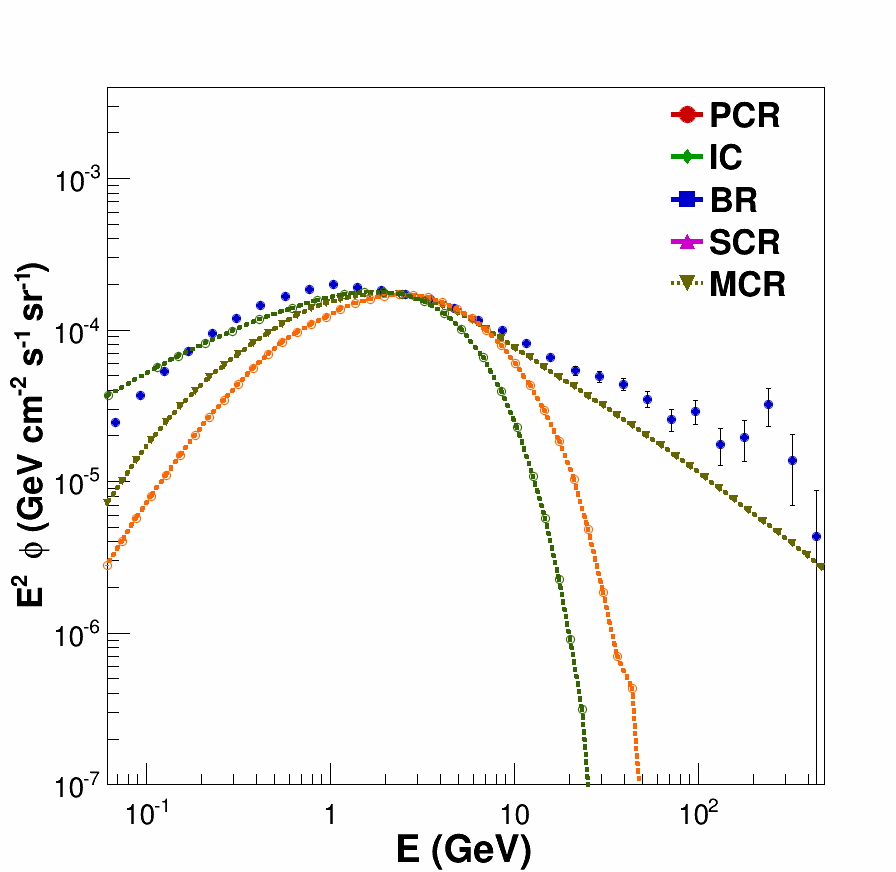
\includegraphics[width=.5\linewidth]{pic/method/excess_comp.png}
% \caption{The three excess component, compared with the data from the central molecular zone.}
% \label{fig:excess_component_comp}
%\end{figure}

\subsubsection{$\pi^0$ production by source cosmic rays (SCR)}

%%% ARTICLE
The proton spectra producing the SCR template can be described by a power law with a spectral index of 2.1, as obtained from the best gamma-ray template fit. The index 2.1 for the SCR template %agrees with the data from the Fermi Bubbles, shown by the data points inside the shaded band in Fig. \ref{fig:proton_spec}; the index 2.1 
is expected from diffuse shock wave acceleration. \todo{cite[60, 61]} 
The source CRs are accelerated, or escape from the galaxy, hence a harder spectrum at high energies compared with propagated CR spectrum is expected.

%The fact that the Fermi Bubbles and the cosmic rays inside sources have the same spectrum strongly suggests that they are connected by point sources providing advective outflows of gas in the Galactic center. \todo{cite[44]}
%%% ARTICLE

\subsubsection{$\pi^0$ production by molecular clouds cosmic rays (MCR)}

%%% ARTICLE
A proton spectrum with broken power-law can be used to parametrize the decreasing gamma-ray emissivity from MCs below 2 GeV. The break can vary from 6 to 14 GeV for different clouds according to the fit. Above the break an optimal spectral index of 2.85 was found to be the same as for the PCR spectrum, as expected if the high energy propagated protons are above a certain magnetic cutoff. Below the break, the spectral index is 0.7, thus providing a significant suppression of protons below the break, as can be seen from Fig. \ref{fig:proton_spec}. This lower break spectral index does not have a strong influence on the fit and therefore is taken to be 0.7.
%Energy losses alone cannot reproduce such a suppression of the proton spectrum below the break, but magnetic cutoffs are able to do so. Such a cutoff is well known from cosmic rays entering the Earth's magnetic field: particles below typically 20 GV entering near the magnetic equator do not reach the Earth, but are repelled into outer space by the geomagnetic cutoff. \todo{cite[62]} The rigidity cutoff of 20 GV is proportional to the magnetic moment. Although the magnetic field near the Earth (0.5 G) is orders of magnitude higher than the typical magnetic fields in dense MCs \todo{cite[63]}, the much larger sizes of MCs - or its substructure of filaments and cloudlets \todo{cite[64]} - yield magnetic moments of the same order of magnitude as the Earth's magnetic moment, so similar magnetic cutoffs are plausible. 
Variations in the magnetic cutoff in MCs are expected from the variations in size and in magnetic field, the latter increasing with MC density. \todo{cite[63]} 
These variations, between 6 and 14 GeV, make the position of the gamma-ray spectrum maximum vary around a few GeV.
%The fit prefers a constant spectral index below the break for all sky directions. Such a constant spectral index is plausible with regular magnetic fields oriented in the disk %\todo{cite[65, 66]} 
%and the "cloudlets" inside MCs %\todo{cite[64]} 
%form magnetic dipole fields. Then the largest cutoff occurs for cosmic rays entering from the halo perpendicular into the cloud for any orientation of the magnetic dipole. For a given entrance angle the cutoff would provide a sharp break, but for an isotropic distribution of entrance angles the break points are smeared. A distribution of break points will provide a slope below the maximum break determined largely by the isotropic distribution of the entrance angles into the disk. Since this distribution is the same for all MCs the slopes below the break will be similar for all MCs, even if the maximum break varies.
%%% ARTICLE

%
%The MCR component is produced by the same process than for PCR, but with a different proton distribution. Due to the magnetic cut-off in MCs, we introduce a break in the proton spectrum between 6 and 14GeV. We leave the index above to 2.85 as for PCR as expected, but we reduce it to 0.7.\\
%
%The magnetic fields around such clouds are not as strong than what we have in the solar system, but the spatial scales are much bigger and could produce such a break. Of course it position may vary from clouds to clouds and it is why we choose to free its position when fitting.\\
%
%This gives us a spectrum peaking around 2GeV.


\subsubsection{Dark matter annihilation (DM)}

%%% ARTICLE
Dark matter particles are expected to annihilate and produce hadrons of roughly twice the WIMP mass, just like in electron-positron annihilation. This would be a large contribution to gamma-rays via $\pi^0$ decays. A smaller fraction of WIMP annihilation can lead to $\tau$ lepton pairs, which can lead to $\pi^0$ production in the hadronic $\tau$ decays. This contribution is expected to be small and is neglected. The DM template can be calculated with the DarkSusy software. \todo{cite[67, 68]} 
An annihilation signal peaking around 2-3 GeV requires a WIMP mass around 50 GeV, as shown in Fig. \ref{fig:norm_excess_component}. 
The DM template falls down to zero for energies above twice the WIMP mass, which make it a softer spectrum than MCR. 
%%% ARTICLE

%
%The DM spectrum is calculated using the DarkSUSY software. Since the initial WIMP mass is not known, we chose to let the fit decide in the CMZ region and fix it to this value in the other regions. The value generally turns around 50GeV, which make the gamma-ray spectrum peak around 2GeV.


\subsubsection{Milli-second pulsars gamma-ray production (MSP)}

The MSP template is directly taken from the Fermi study \todo{cite paper}. It simulates the emission of 1700 milli-second pulsars with different energies around the galactic center.
The high energy shape of the spectrum closely resemble the DM template, but the main difference with DM and MCR is for low energies. Indeed, below 1 GeV, the MSP template is a lot softer and this feature makes it discernible from MCR and DM.

\subsubsection{Isotropic component}

\begin{figure}
 \centering
 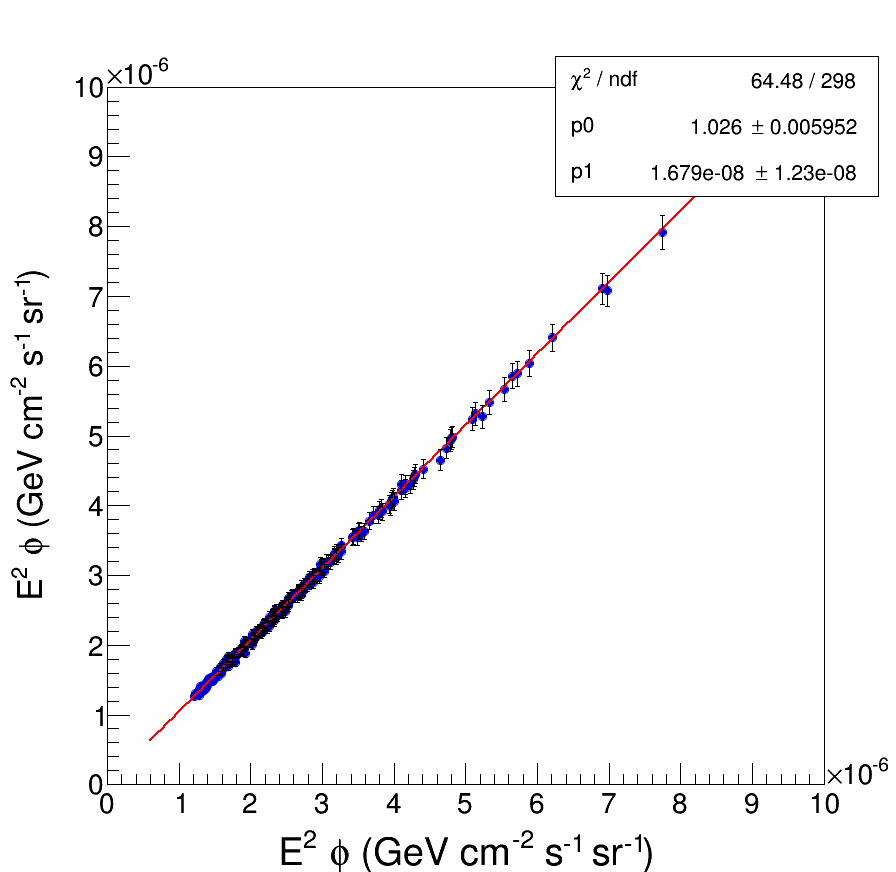
\includegraphics[width=.5\linewidth]{pic/method/iso_calibration.png}
 \caption{The fitted flux versus the observed flux data in every region of the sky for a given energy of 1 GeV. A linear fit is performed to find the offset p1 at the vertical axis. This number represents the amount the isotropic component shifts the data in all cones. Once this is done for every energy bin, the offset is added to the previous isotropic template and the process is repeated until convergence. }
 \label{fig:iso_calibration}
\end{figure}


%%% ARTICLE
The isotropic template represents the contribution from the isotropic extragalactic background and hadron mis-identification. Its spectral shape and absolute normalization are provided within the Fermi software \todo{cite[51]}, but it was redetermined for the analysis as follows.
A first fit of the data in regions outside the bubbles and the galactic disk using the isotropic template from the Fermi software is produced as an initial estimate. This fit takes into account all components of the best fit available.
If one plots the total observed gamma-ray flux versus the fitted flux in the various cones in a certain energy bin, one expects a linear relation crossing the origin if the isotropic flux is estimated correctly (See Fig. \ref{fig:iso_calibration}). However, if the isotropic contribution is either too low or too high, an offset at the origin is introduced in the linear relation. Since the isotropic component is by definition the same for all cones for a given energy, this offset can be subtracted from the Fermi template to improve the fit. 
%An example of such a fit is shown in Figure \ref{fig:iso_calibration} for an energy bin between \todo{3.7-5.2 GeV}. 
Once the offset is determined for each energy bin and subtracted from the original template, the process is repeated until the offset converges to zero.

%The linear relation between data and fit is always supposed to have a slope of one, or the process does not converge.
\todo{maybe add pictures of the iso template through different steps}
%The resulting template in our analysis has deviations from the Fermi template up to $35\%$ above 2 GeV, as shown in the insert of \ref{fig:iso_calibration}.
%%% ARTICLE

\newpage
\section{Fitting method}
%My method:
%	-Spectral templates fitted to the data
%		-independant spatial cones on the entire sky (usually 797 for optimized sizes)
%		-minimum chi2 fit using ROOT for every cone
%		-Benefits
%			-energy related features
%			-only a few degrees of freedom -> Well constrained fit (5(or 6) dof against 21-30 points)
%		-Downside:
%			-No spatial templates. (only the isosky)


The fitted data can be seen as a data cube whose dimension are longitude, latitude and energy. The finest spatial grid is divided in $720 \times 360$ cones of $ 0.5^\circ \times 0.5^\circ $. Every cone contains 30 energy bins. This allows to treat different portions of the sky independently of one another.
(((Since the cones do not have the same solid angle and the statistics in a small binning is low, the grid is more often composed of 797 bins of different sizes, bigger at the poles and smaller near the equator. This allows for higher statistics in lower flux regions and where a high spatial resolution is not needed (i.e. at high latitudes). In the same time, the equator and the GC have a lot more counts and can be treated in a smaller binning. This binning is faster to compute than a regular grid with an good enough output quality to study the results.)))

The fit uses a certain number of components (three at least) each corresponding to a certain phenomenon and described earlier. They all have certain energy spectra that can vary with the position in the sky in the case of IC (See Fig. \ref{fig:norm_spectra}).

The fits are done for every bin independently. After choosing the templates used for the fit, their scaling factor is the only degree of freedom allowed.  Using a ROOT TVirtualFitter object, every template is scaled up or down until its sum comes the closest to the data.
Mathematically, the minimum distance between the model and the data is found when the $\chi^2$ value is lowest. It is calculated as follows:

\begin{equation}
\chi^2 = \sum_{i=1}^{30} \left[ \frac{ \left( D_i - \sum_{j=1}^{n} \left[ (n_jT_{ij})^2 \right] + iso \right) ^2}{\sigma_i^2} \right]
\end{equation}

where:
\begin{itemize}
\item $D_i$ is the data flux in the $i^{th}$ energy bin.
\item $n_j$ is the scaling factor for the $j^{th}$ model component.
\item $T_{ij}$ is the model flux of the $j^{th}$ in the $i^{th}$ energy bin.
\item $\sigma_i$ is the geometric mean of the statistical and systematical error of the Fermi data point $i$.
\end{itemize}

The MCR break position does not vary in a single fit. A fit is done for different values of the MCR break independently, and the one with the smallest $\chi^2$ is kept. This break position is not counted as a degree of freedom in the fit.

The fit is very well constrained with only five or six degrees of freedoms depending on the model against 30 data points. A useful value is the $\chi^2 / d.o.f$ where $d.o.f = \#data\ points - \#free\ parameters - 1$. Thus, if a model describes data completely within its uncertainty, $\chi^2 / d.o.f = 1$, making the comparison between different fits easier. This rescaling will be applied every time when speaking about $\chi^2$ in the rest of the discussion, except if explicitly told. 
The closest a $\chi^2$ value is to one, the better the model follows the data. The higher it gets, the lower the quality of the fit. It can also happen that it gets lower than one. This can happen when the error bars on the data are too big.


Since every bin is fitted independently, it is not possible to implement a spatial template, i.e. where the spatial shape of a component would be fixed in advance. For example a component with a spherical distribution around the GC, as has been done in other works \todo{cite}. It is used to let the fit find reasonable shapes by itself, only using the $\chi^2$ minimization technique.

%\section{Introduction of results}

This fitting method offers many ways to look at the results, depending on the interest. It is possible to produce flux maps of each component to study their spatial shapes at different energies. This can for example show a correlation between a certain template and a galactic feature such as the disk or the bubbles. Another way is to create a spectrum of one cone to look at the relative quantity of every template at different energies. This can put into evidence issues within the models and help improve the spectral shape of the components.

The first step when testing a new model is to see if it can reproduce results of previous studies. Only once it works and can be confidently used, can it produce new results.

%The next chapter will describe these results, first reproducing old studies, and 

%Recreation of previous studies (GC excess, problems).\\
%Introduction of new component to take care of those problems (SCR for high energies, MCR, Dm or MSP for 2GeV excess)


%%	-Weniger plots
%%		-study of spectra slope between 0.3 and 2 GeV
%%	-Specklings
%%		-Study of symmetry
%%	-Comparison with CO map

%% ==================
\chapter{Results}
\label{ch:results}
%% ==================
%
%My results:

\section{Recreating previous results}
\label{sec:results_recreating_prev_res}
%	-Only 3 original components
%		-Spherical excess
%		-very bad chi2 in disk and bubbles

Introduce the weniger plots here (or in the state of the research?) to show excess in GC.
\begin{figure}[h]
  \centering
  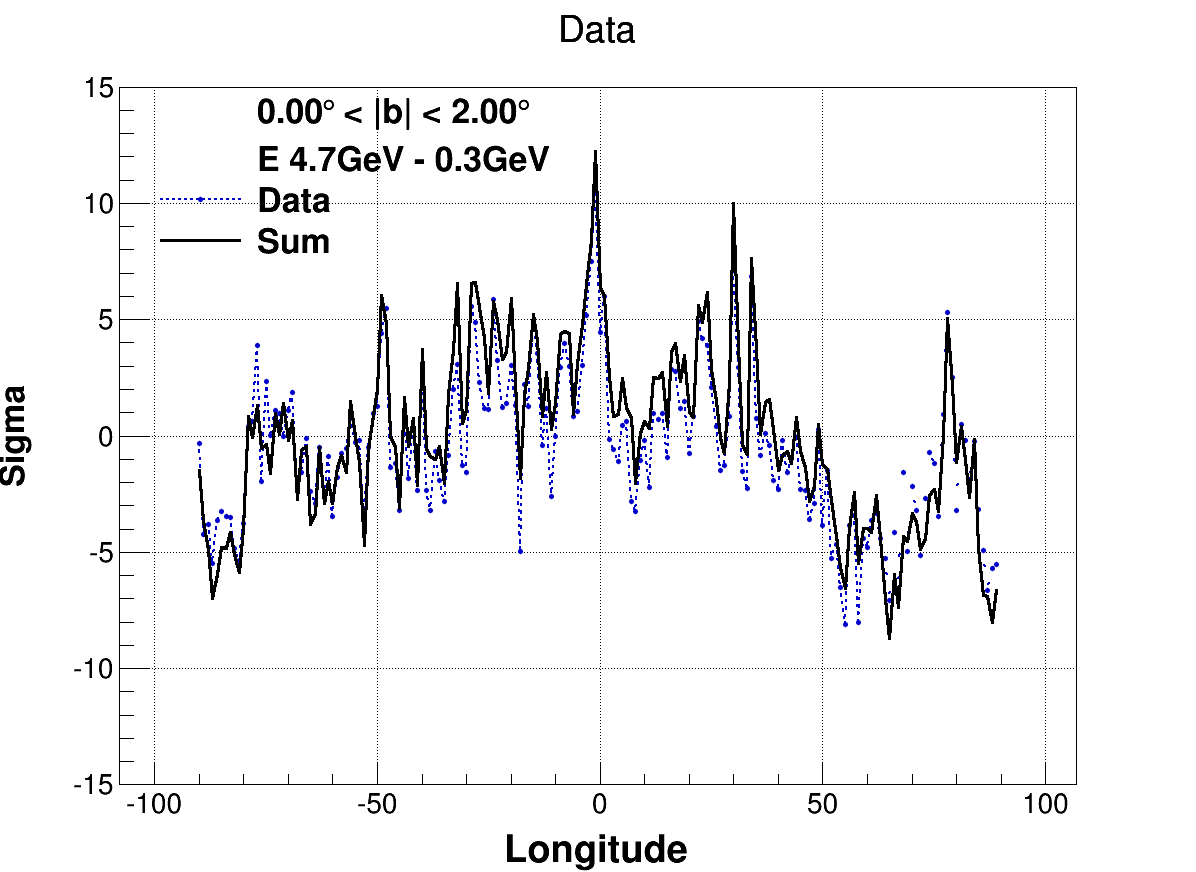
\includegraphics[width=.5\linewidth]{pic/results/Weniger_SUM_b0-2_E4,7-0,31GeV.png}
  \caption{Some weniger plots to show the GC excess}
  \label{fig:weniger_plot}
\end{figure}


\begin{figure}[h]
  \centering
  \begin{minipage}[h]{0.45\textwidth}
  	\centering
	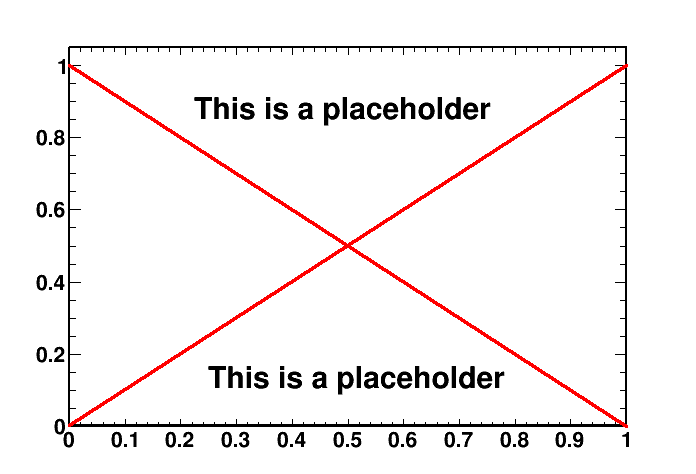
\includegraphics[width=1.\linewidth]{pic/dummy.png}
  	\subcaption{Picture of GC excess as fitted previously (https://arxiv.org/pdf/1110.0006.pdf?)}
  	\label{fig:original_GC_excess}
  \end{minipage}
  \hfill
  \begin{minipage}[h]{0.45\textwidth}
	  \centering
	  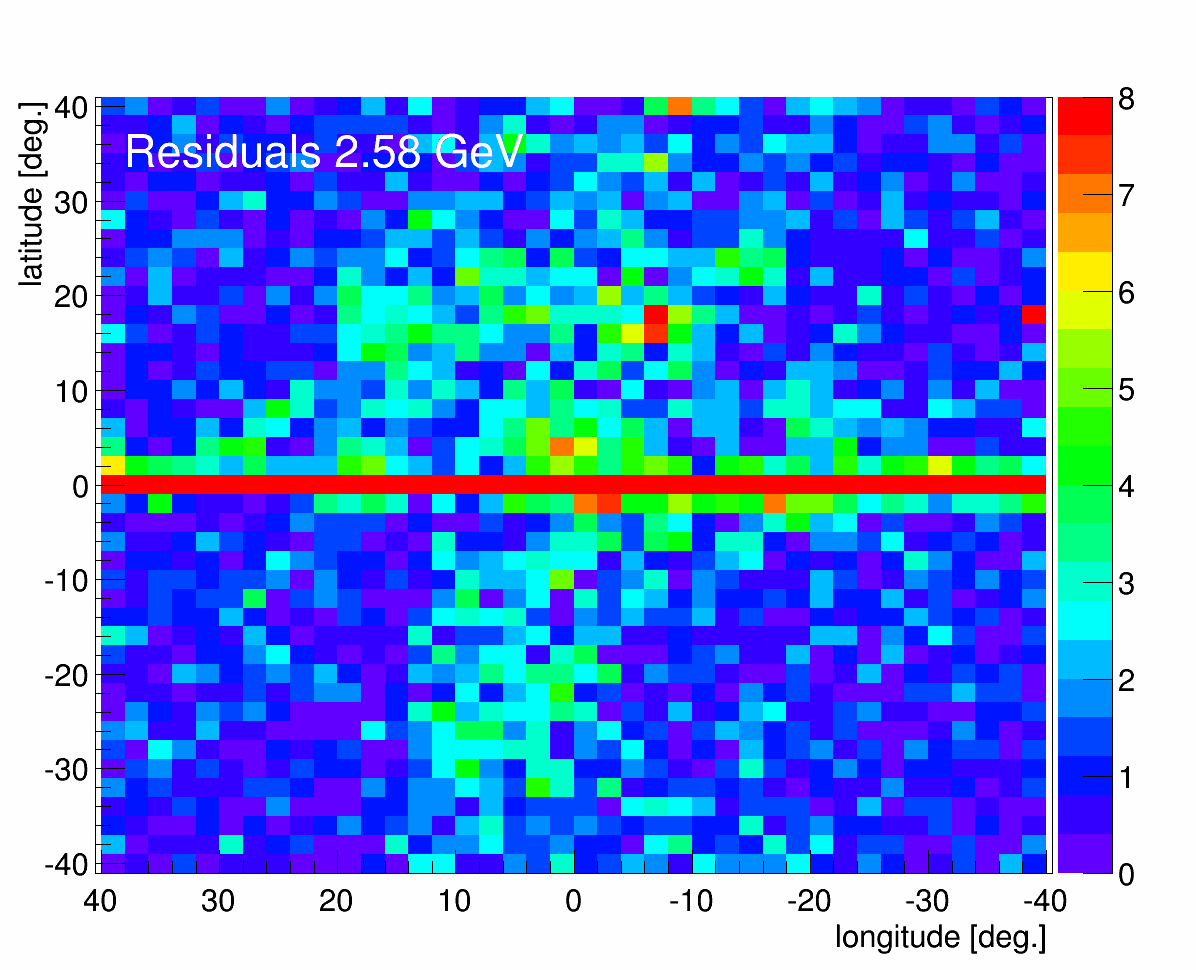
\includegraphics[width=1.\linewidth]{pic/results/BKGonly_halo_residuals.png}
	  \subcaption{Picture of GC excess as fitted by us}
	  \label{fig:our_GC_excess}
  \end{minipage}
  \caption{Picture of the GC excess as obtained previously and with our fit}
  \label{fig:GC_excess}	 
\end{figure}

Before trying to upgrade the current model, it is important to make sure it can be recreated starting from the same parameters. Fig. \ref{fig:original_GC_excess} shows the results of a fit using only the background components (PCR, IC and BR). The shape and intensity of the previously observed excess are found \todo{cite}. Excluding the galactic disk for latitudes below two degrees, the excess extends to $30\circ$ in all directions from the GC.

\begin{figure}[h]
  \centering
  \begin{minipage}[h]{0.45\textwidth}
  	\centering
	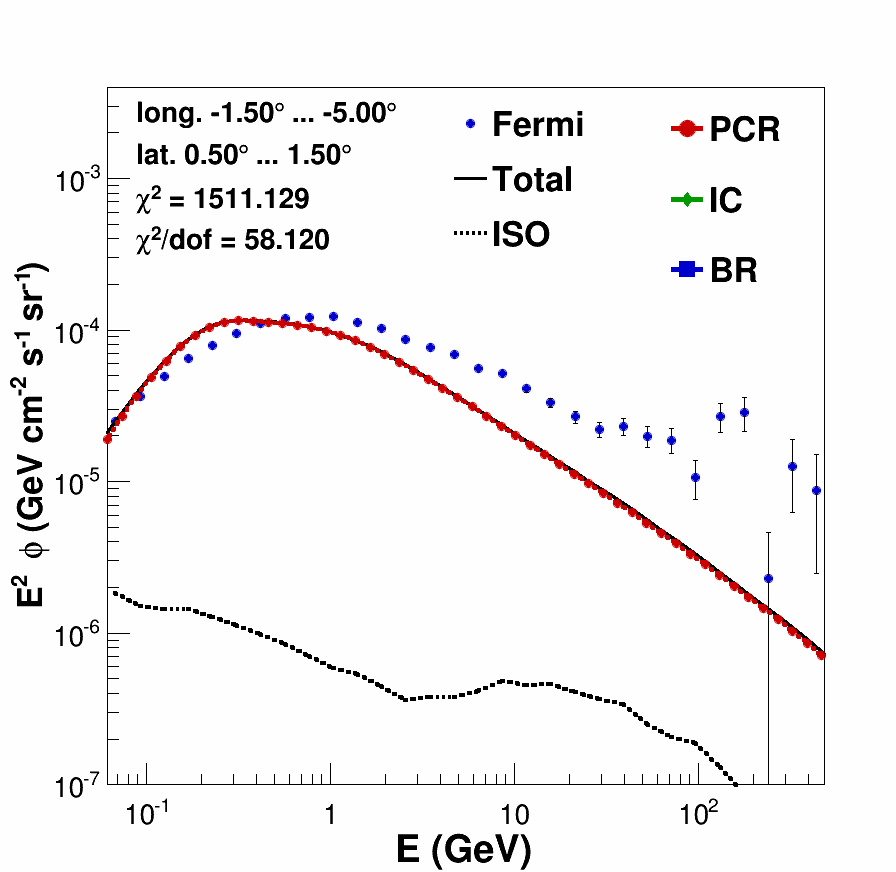
\includegraphics[width=1.\linewidth]{pic/results/BKGonly_CMZ.png}
  	\subcaption{Picture background only spectra with bad fit (high energies too hard)}
  	\label{fig:bkgd_only_spectrum}
  \end{minipage}
  \hfill
  \begin{minipage}[h]{0.45\textwidth}
	  \centering
	  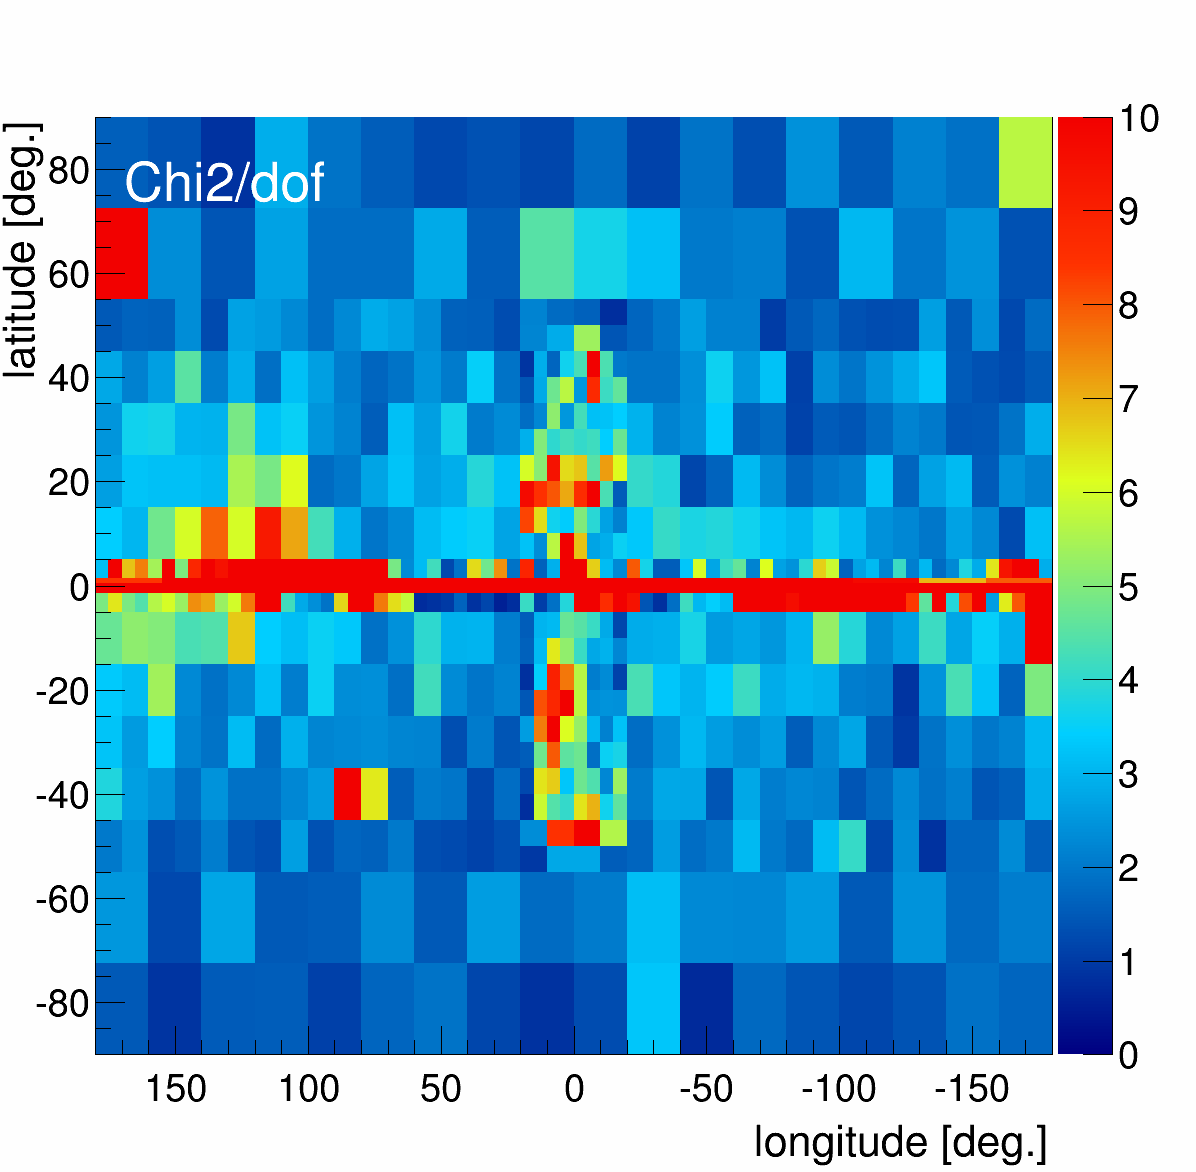
\includegraphics[width=1.\linewidth]{pic/results/chi2_distribution_BKGonly.png}
	  \subcaption{Chi2 Distribution for BKGonly fit}
	  \label{fig:MKGonly_chi2Distribution}
  \end{minipage}
  \caption{Example of fit and chi2 map of BKG only fit}
  \label{}	 
\end{figure}


Looking at the $\chi^2$ skymap (Fig. \ref{fig:original_GC_excess}), the bubbles and the disk appear clearly in red, showing a high $\chi^2$ value. The fit does not give proper results in those regions, with the high energy part of the spectrum not described by the three background templates. On the other hand, outside these regions, the fit is works better with a $\chi^2$ not much higher than three. This is not perfect, but in comparison with the disk, it is undeniably better.
Overall, the results are expected and confirm that the model is incomplete. The introduction of a new template like SCR should help improve the fit.


%where the high energy spectrum is harder (see Fig. \ref{fig:bkgd_only_spectrum}). In this region, the PCR spectrum falls off too quickly, and the IC spectrum which usually takes care of high energies is blocked by the low energy flux drop.


%I was able to recreate a more or less spherical excess in GC around 2GeV.\\
%Bad fit in disk and bubbles as expected.
%Two problems :
%\begin{itemize}
%\item Spectrum too hard at high energies
%\item Excess around 2GeV
%\end{itemize}


\section{Introducing SCR}

\begin{figure}[h]
  \centering
  \begin{minipage}[h]{0.45\textwidth}
  	\centering
	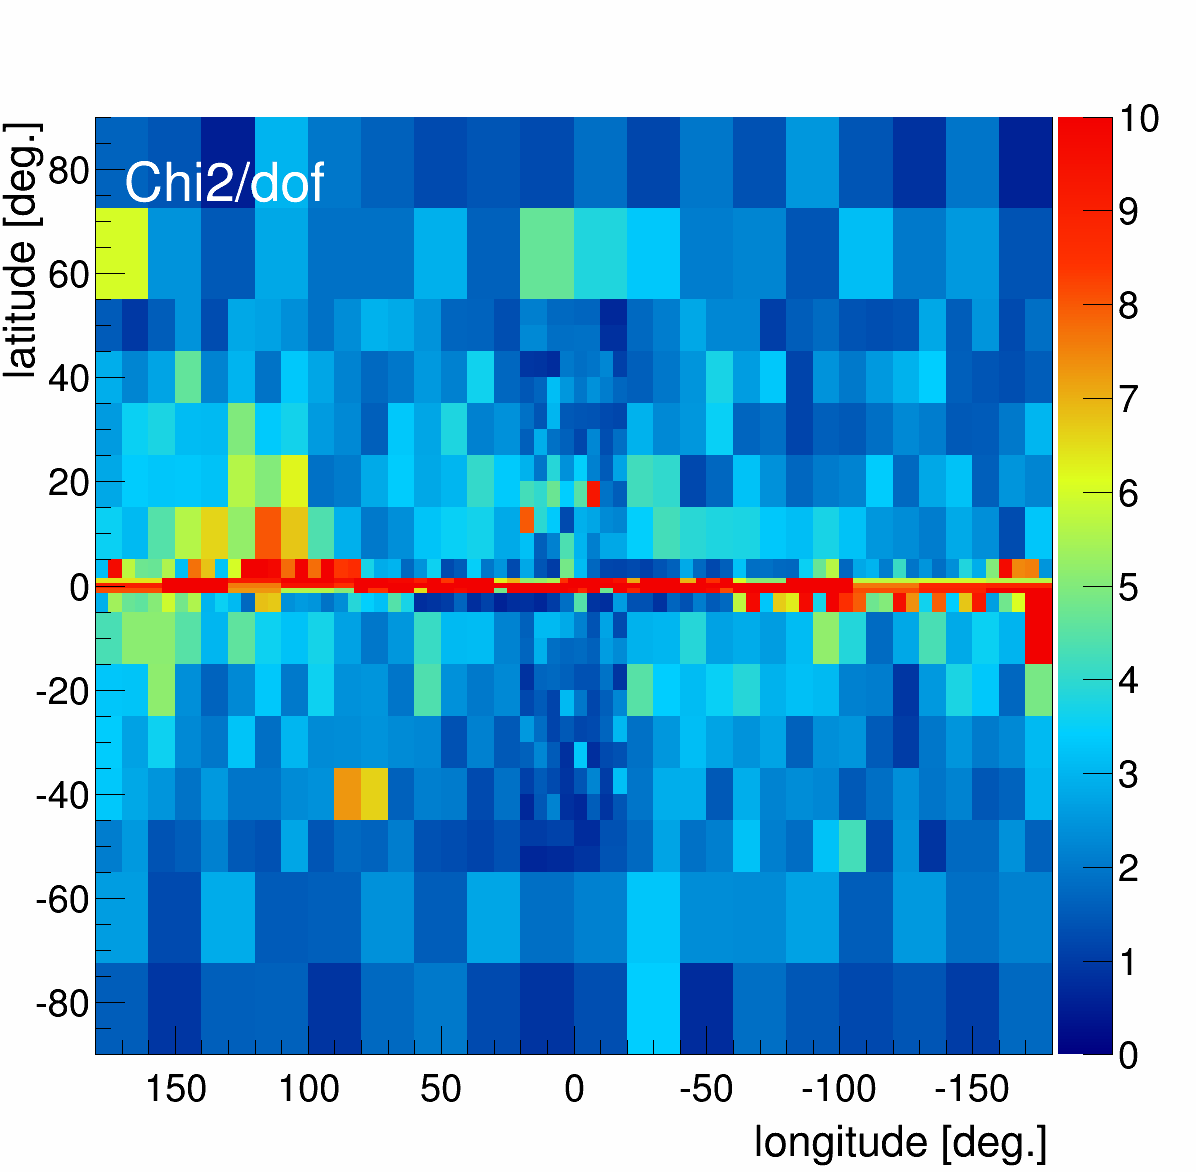
\includegraphics[width=1.\linewidth]{pic/results/SCRonly_Chi2Distribution.png}
  	\subcaption{Chi2 distribution of SCR only fits.}
  	\label{fig:SCRonly_fit}
  \end{minipage}
  \hfill
  \begin{minipage}[h]{0.45\textwidth}
	  \centering
	  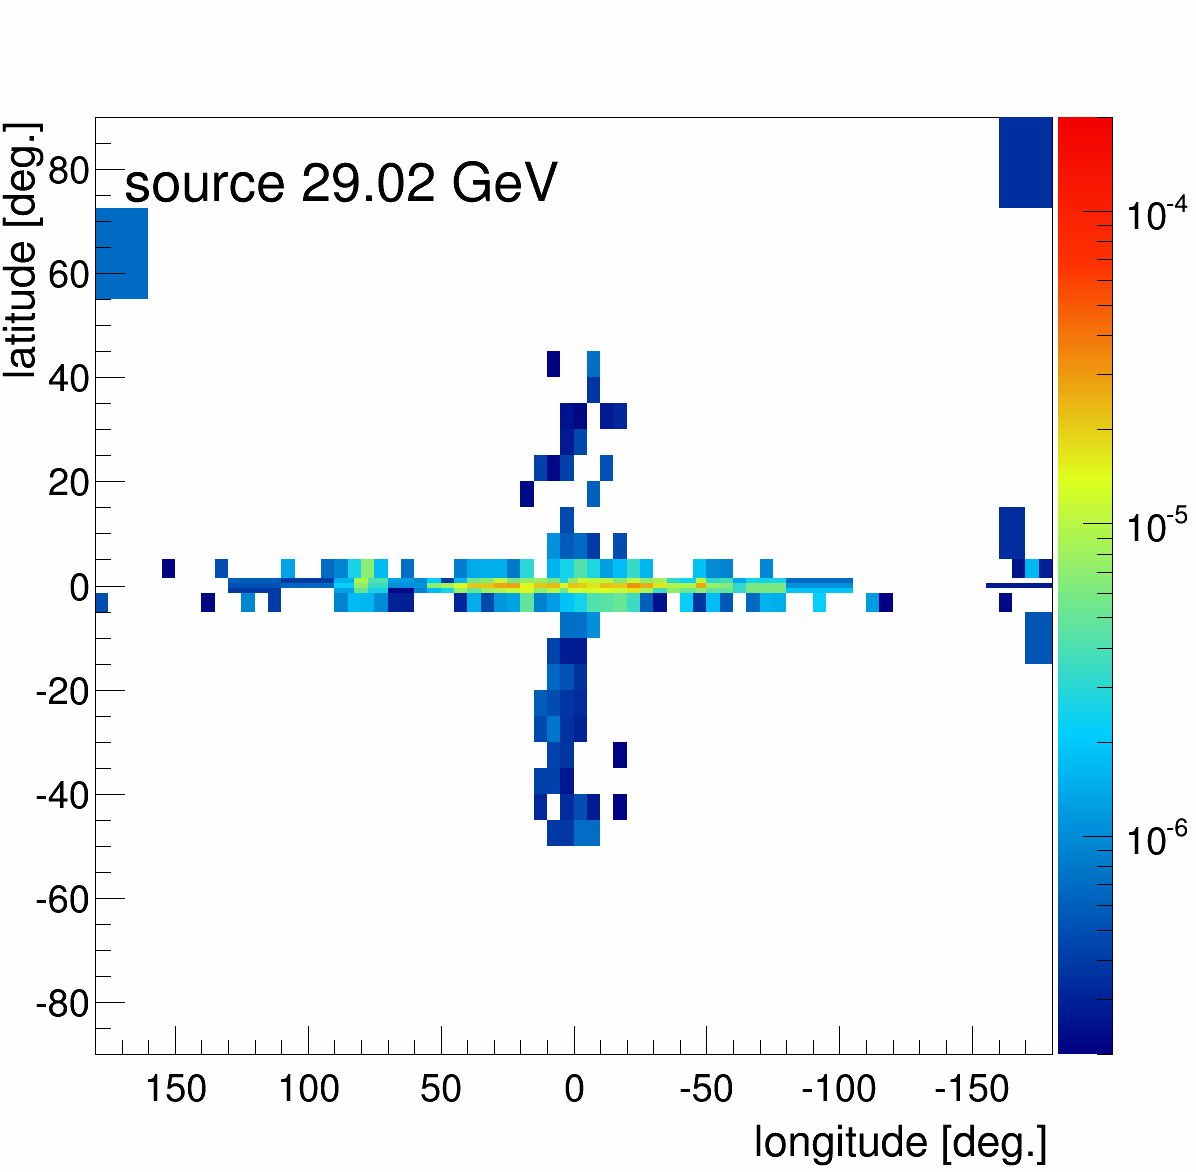
\includegraphics[width=1.\linewidth]{pic/results/SCR_flux_distribution_bin20.png}
	  \subcaption{Flux distribution of SCR only fits.}
	  \label{fig:BKGonly_bubble_spec}
  \end{minipage}
  \subcaption{Source results}
  \label{fig:SCRonly_distributions}
\end{figure}


After introducing the SCR template, a clear improvement can be noted in the $\chi^2$ distribution (see Fig. \ref{fig:SCRonly_fit}). The bubble shape that was delimited before by a bad $\chi^2$ zone has now disappeared. Even if the fit is still not perfect everywhere, the improvement is significant. For example, the disk is still not fitted properly, with very high $\chi^2$ values. Some structures can be seen along the disk for absolute longitudes over $90\circ$

\begin{figure}[h]
  \centering
  \begin{minipage}[h]{0.45\textwidth}
  	\centering
	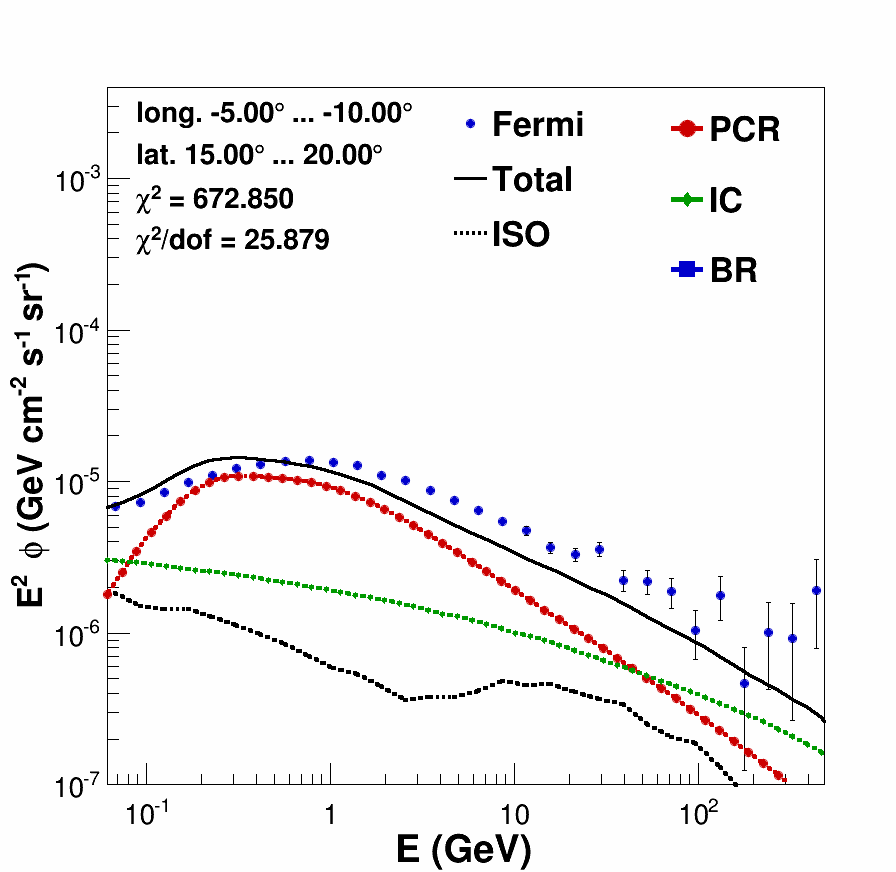
\includegraphics[width=1.\linewidth]{pic/results/bkgdonly_spectra_bubble_example.png}
  	\subcaption{Spectrum from a bubble with SCR only and background only.}
  	\label{fig:SCRonly_bubble_spec}
  \end{minipage}
  \hfill
  \begin{minipage}[h]{0.45\textwidth}
	  \centering
	  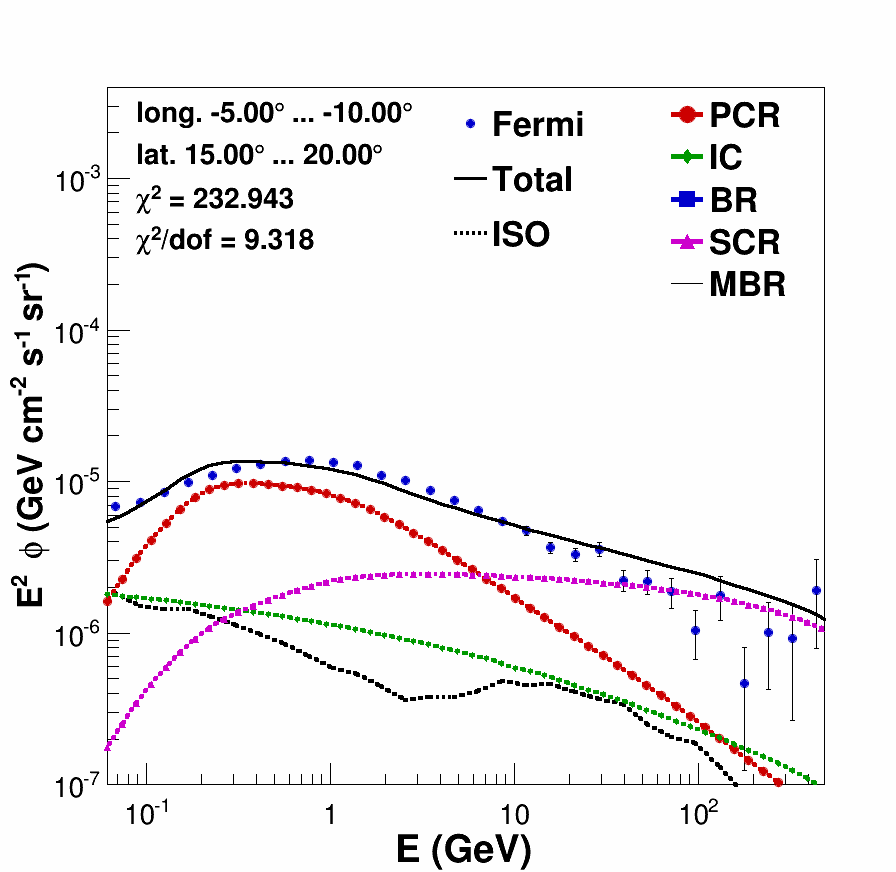
\includegraphics[width=1.\linewidth]{pic/results/SCRonly_spectra_bubble_example.png}
	  \subcaption{Spectrum from a bubble with background models only and background only.}
	  \label{fig:BKGonly_bubble_spec}
  \end{minipage}	 
\end{figure}

The SCR template is present only in the disk and the bubbles \todo{add fig}, as expected since it represents the point sources and CR that did not diffuse in the disk. The high energy parts (above 100 GeV) of the spectra are dominated by SCR.

\todo{chack if the GC excess still exist, if yes, talk about it. Then introduce the excess components}



%From Fig. \ref{fig:SCRonly_bubble_spec} and \ref{fig:SCRonly_bubble_spec} we see the role of the SCR template at high energies, taking care of the high flux. It also permits a better fit of low energies by PCR and IC since they do not have to be everywhere at the same time.

%\todo{Here the bad chi2 comes from 0.1GeV region, where the PCR template does not fit the data. not from the 2GeV excess.}
%A problem still remains in the disk and diffuse regions around the galactic anticenter. 



\section{Introducing SCR and MCR}
%	-Introduction of SCR and MCR
%		-very good chi2 in disk and bubbles
%		-spatial shapes of comps
%			-IC sperical (as expected) but depletion in disk
%			-BR low in bubbles replaces IC in disk
%			-PCR OK but low in disk
%			-MCR follows CO map, take place of PCR in disk
%			-SCR follows bubble structure

\begin{figure}[h]
  \centering
%   \todo{May have to change it if we change the bckground model} 
  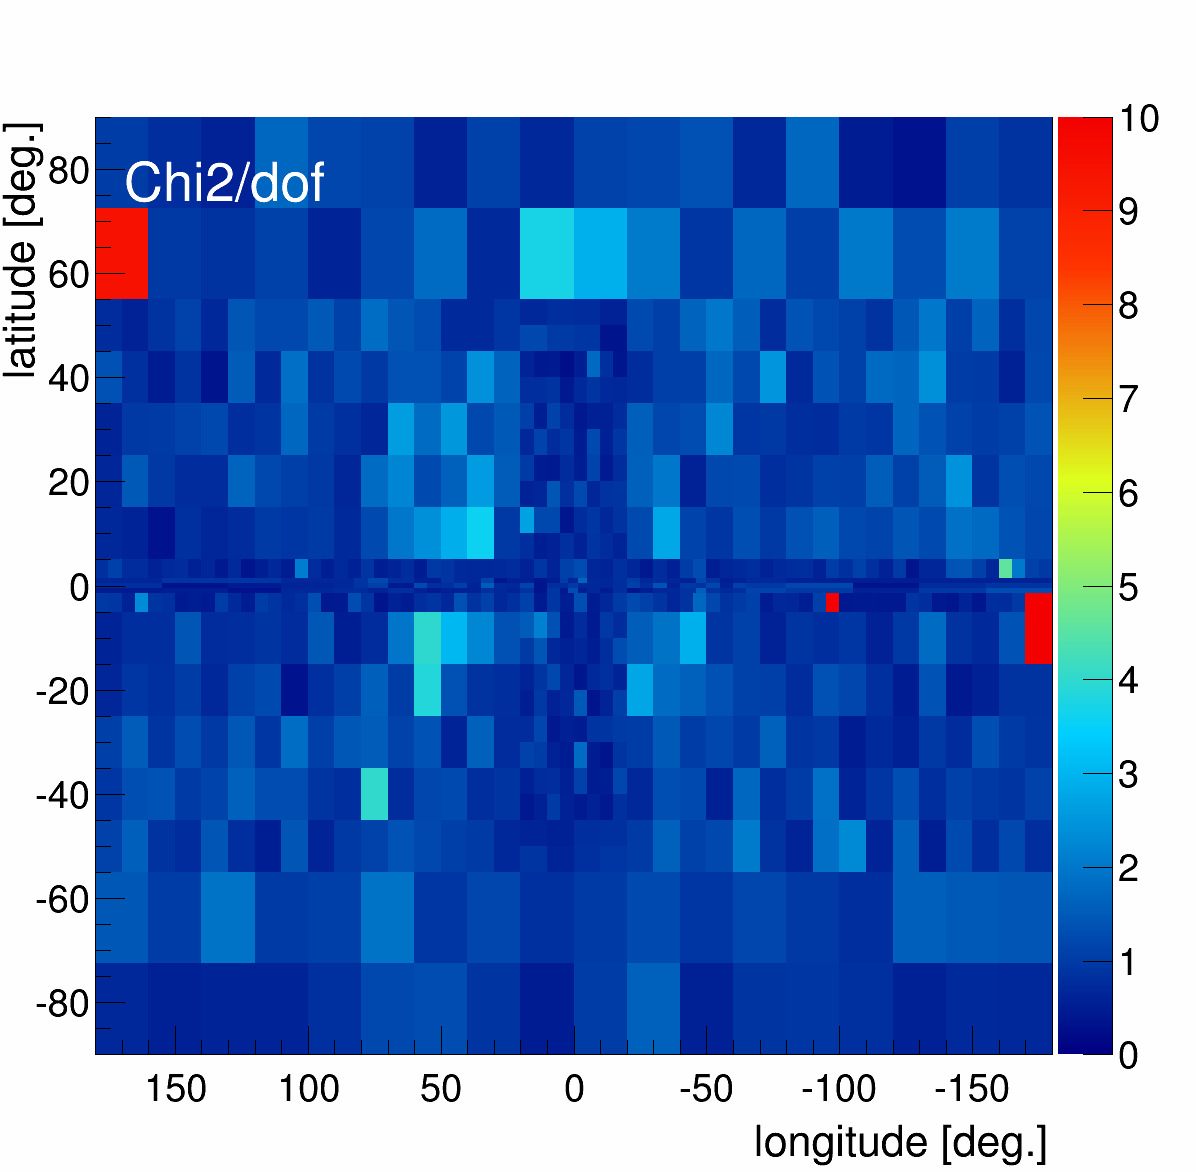
\includegraphics[width=.5\linewidth]{pic/results/MCRonly_chi2Distribution.png}
  \caption{Chi2 maps of MCRonly fits compared to background only}
  \label{fig:MCRonly_chi2Distribution}
\end{figure}
%First obvious thing is the good chi2 in the disk and bubbles.\\

As shown on Fig. \ref{fig:MCRonly_chi2Distribution}, the addition of a new template improve significantly the $\chi^2$ distribution in all directions. The bubbles and the disk structures are not visible anymore.

Three dots appear to have a really high $\chi^2$, but that is only due to the point source subtraction that is not perfect (see Chapter \ref{sec:Data_origin}).

\begin{figure}[h]
  \centering
  
  \begin{minipage}[h]{0.45\textwidth}
	  \centering
	  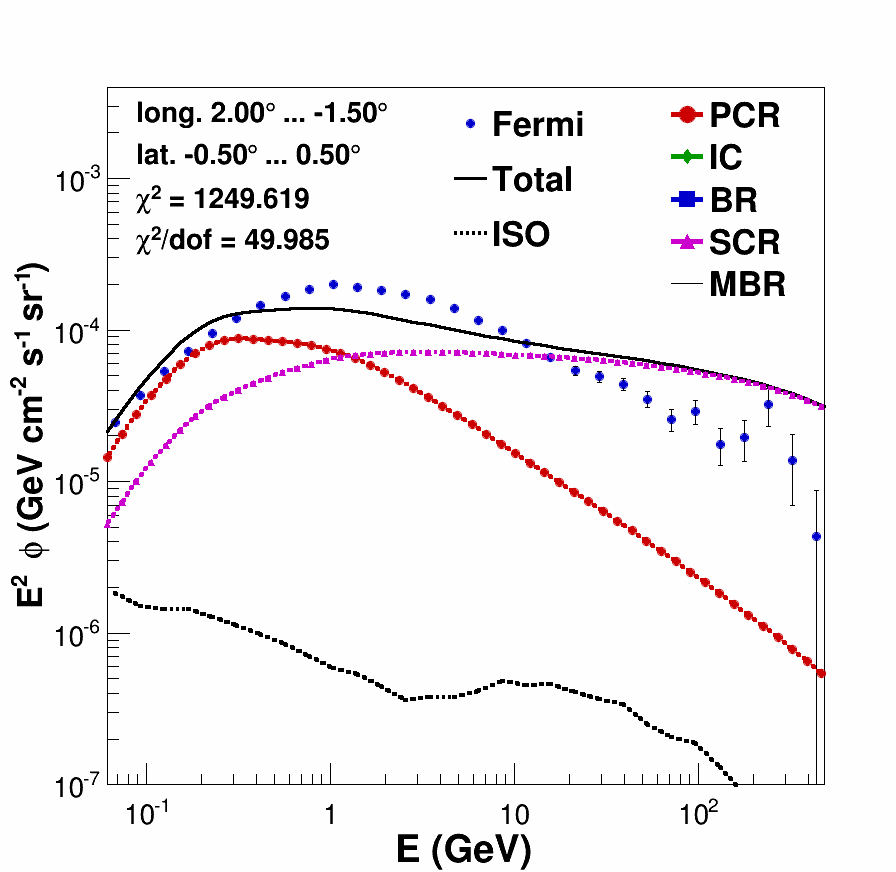
\includegraphics[width=\linewidth]{pic/results/SCRonly_CMZ.png}	  
  	  \subcaption{SCR fit in the CMZ region}
	  \label{fig:SCRonly_CMZ}
  \end{minipage}
  \hfill
  \begin{minipage}[h]{0.45\textwidth}
	  \centering
	  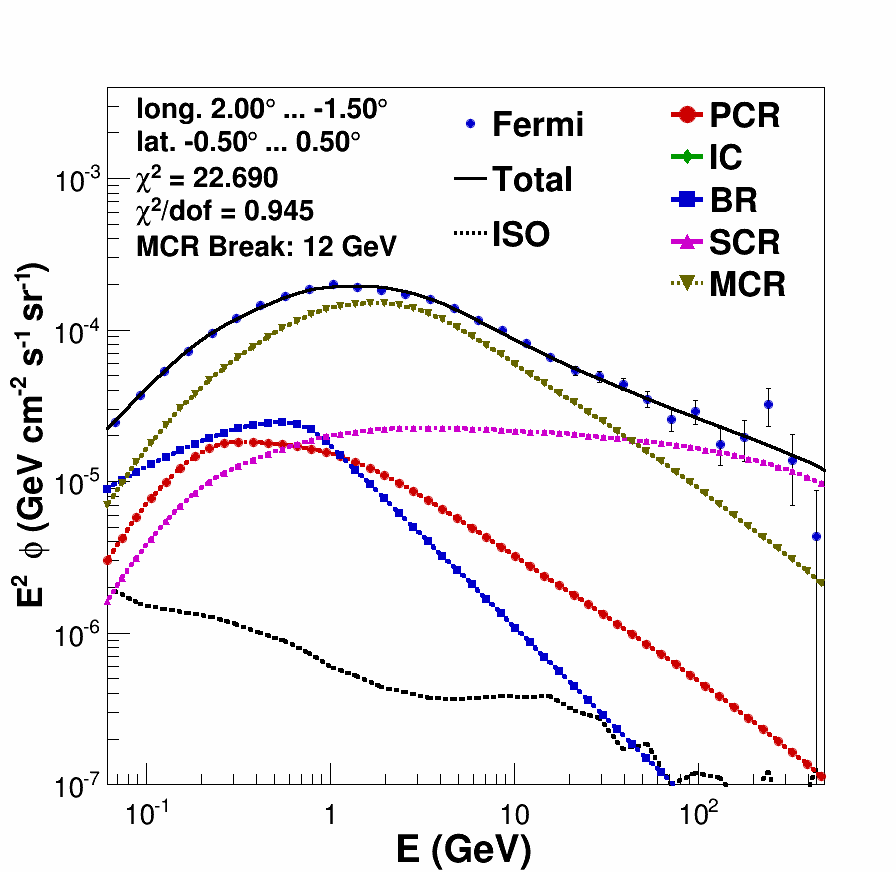
\includegraphics[width=\linewidth]{pic/results/MCRonly_CMZ.png}
	  \subcaption{MCR fit in the CMZ region}
  	  \label{fig:MCRonly_CMZ}
  \end{minipage}
  \label{fig:MCR_vs_SCRonly_CMZ}
\end{figure}

Fig. \ref{fig:MCR_vs_SCRonly_CMZ} shows the central molecular zone (CMZ) fitted with and without the MCR component. The gas density is very high in this region, hence it is the first region where we would expect the MCR emission to be present, if not dominant compared to PCR. Indeed the fit chooses this configuration, with the MCR template dominating all the others and we can directly see the improvement in the MCR fit. The energies around 2GeV had a clear excess that the four components of the SCR fit could not account for. The MCR template peaking in this region, it comes in very handy and fill this gap, leaving the SCR template taking care of the high energies and PCR and BR for the low energies. \todo{Why isn't there IC? -> Wait to see if we change the models}

\newpage
\begin{figure}[h]
  \centering
  \begin{minipage}[h]{0.45\textwidth}
  	\centering
	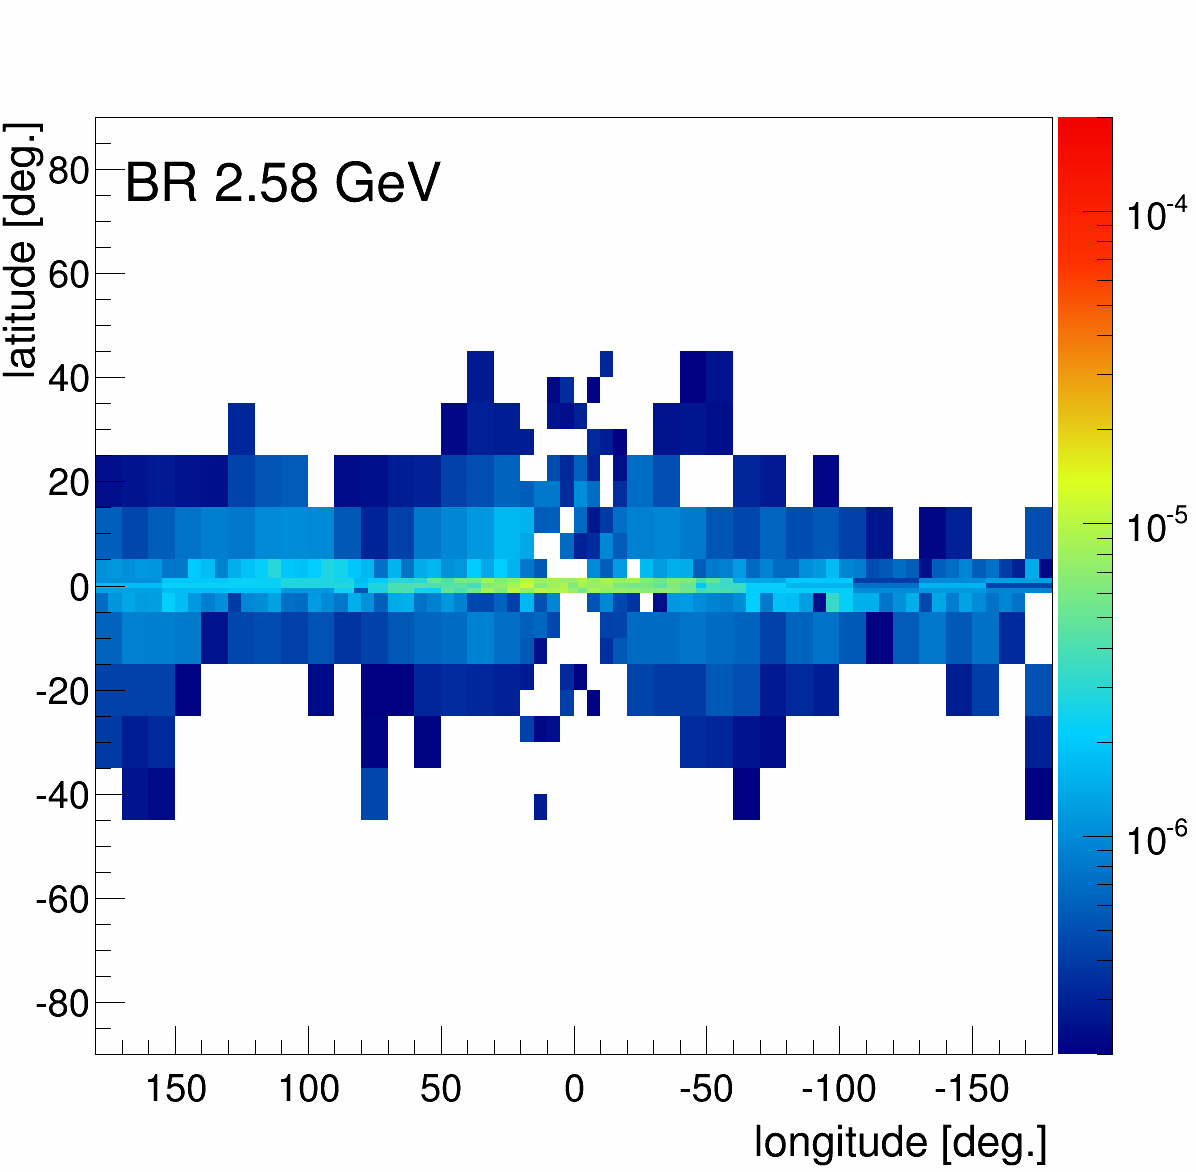
\includegraphics[width=1.\linewidth]{pic/results/MCRonly_BR_fluxE12_skymap.png}
  	\subcaption{Flux distribution of bremstrahlung (BR)}
  	\label{fig:MCRonly_skymap_BR}
  \end{minipage}
  \hfill
  \begin{minipage}[h]{0.45\textwidth}
  	\centering
	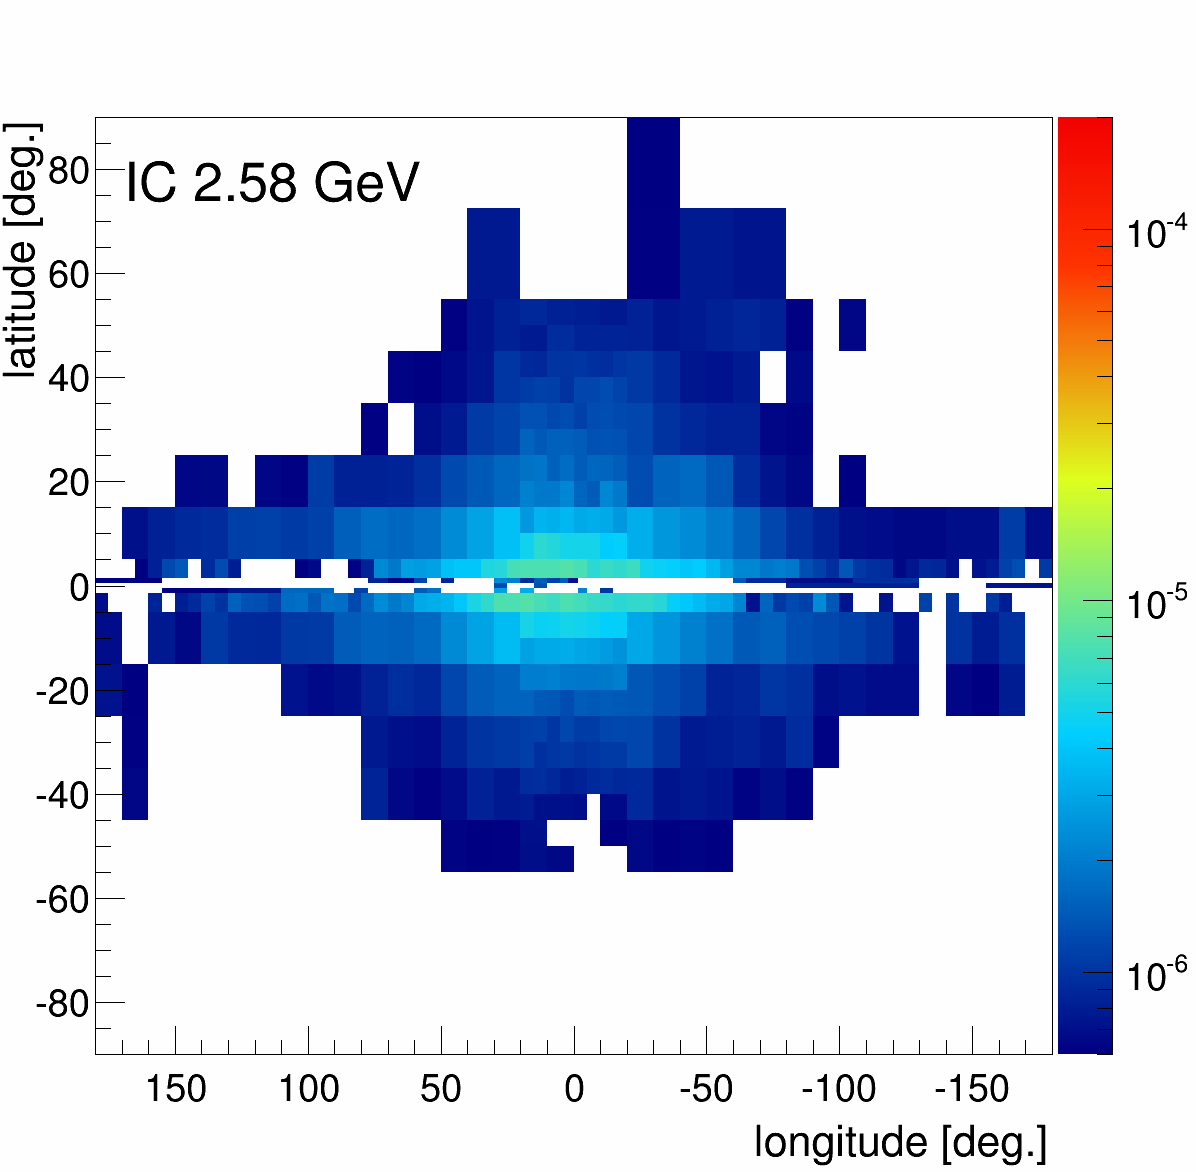
\includegraphics[width=1.\linewidth]{pic/results/MCRonly_IC_fluxE12_skymap.png}
  	\subcaption{Flux distribution of inverse compton (IC)}
  	\label{fig:MCRonly_skymap_IC}
  \end{minipage}
  \hfill
  \begin{minipage}[h]{0.45\textwidth}
  	\centering
	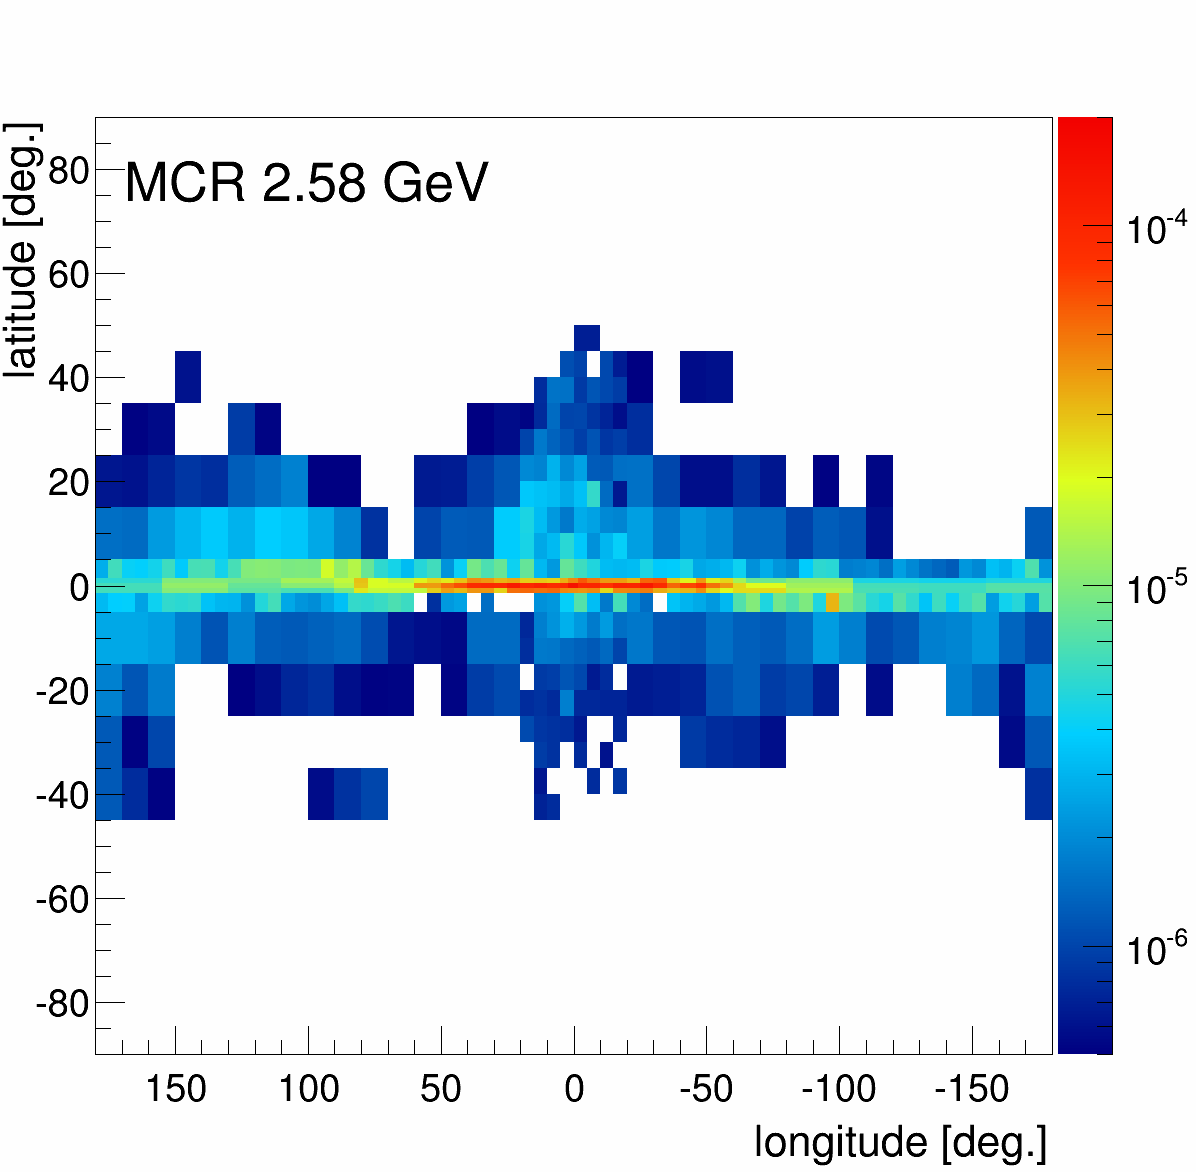
\includegraphics[width=1.\linewidth]{pic/results/MCRonly_MCR_fluxE12_skymap.png}
  	\subcaption{Flux distribution of MCR}
  	\label{fig:MCRonly_skymap_MCR}
  \end{minipage}
  \hfill
  \begin{minipage}[h]{0.45\textwidth}
  	\centering
	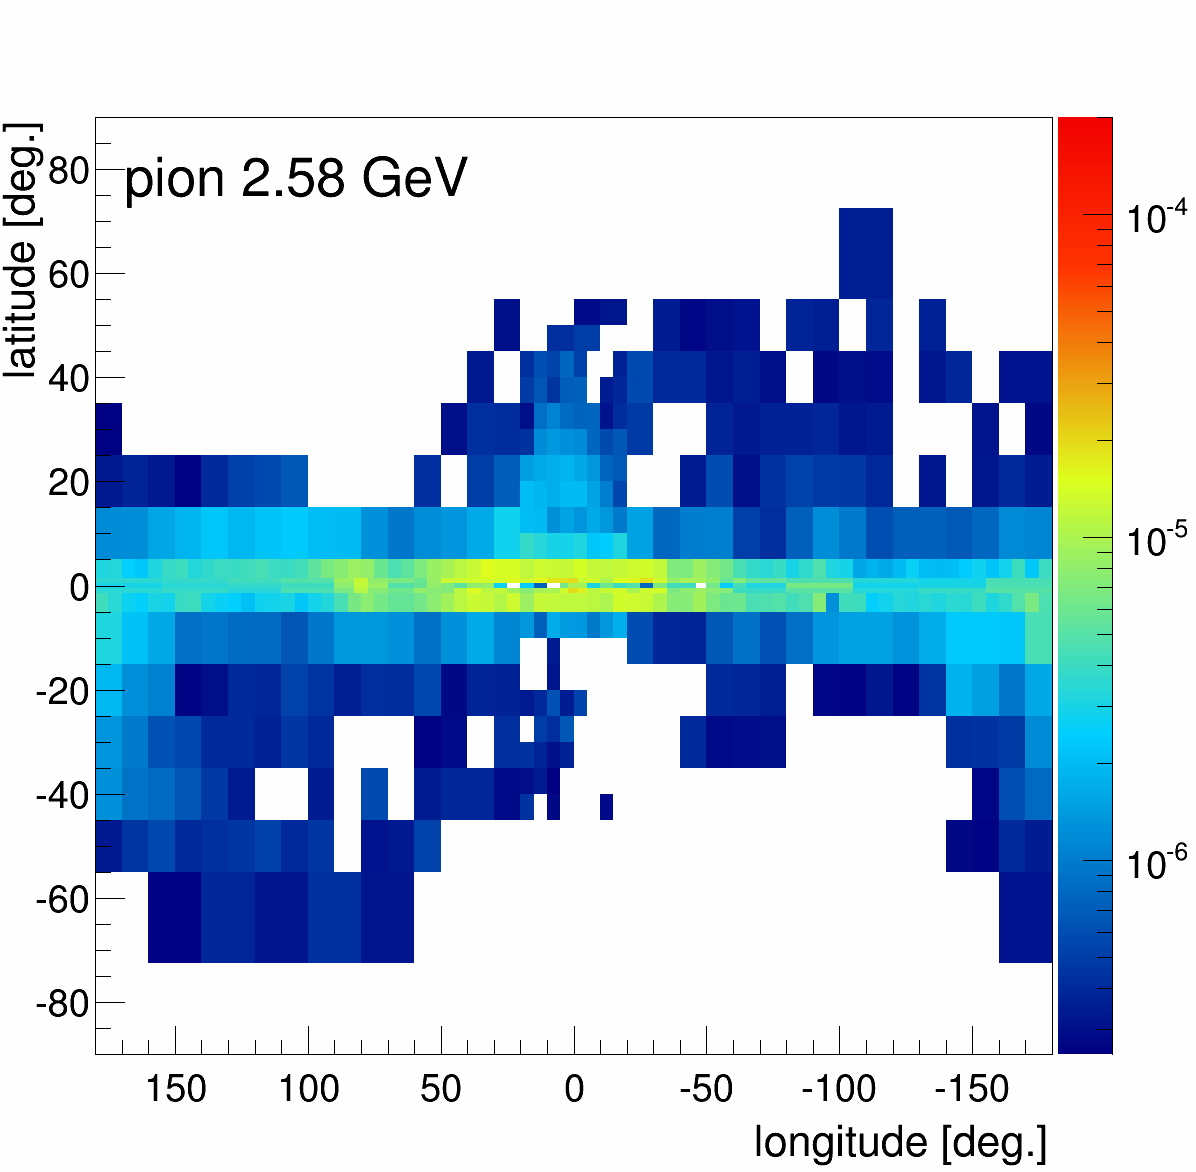
\includegraphics[width=1.\linewidth]{pic/results/MCRonly_PCR_fluxE12_skymap.png}
  	\subcaption{Flux distribution of PCR}
  	\label{fig:MCRonly_skymap_PCR}
  \end{minipage}
  \hfill
  \begin{minipage}[h]{0.45\textwidth}
  	\centering
	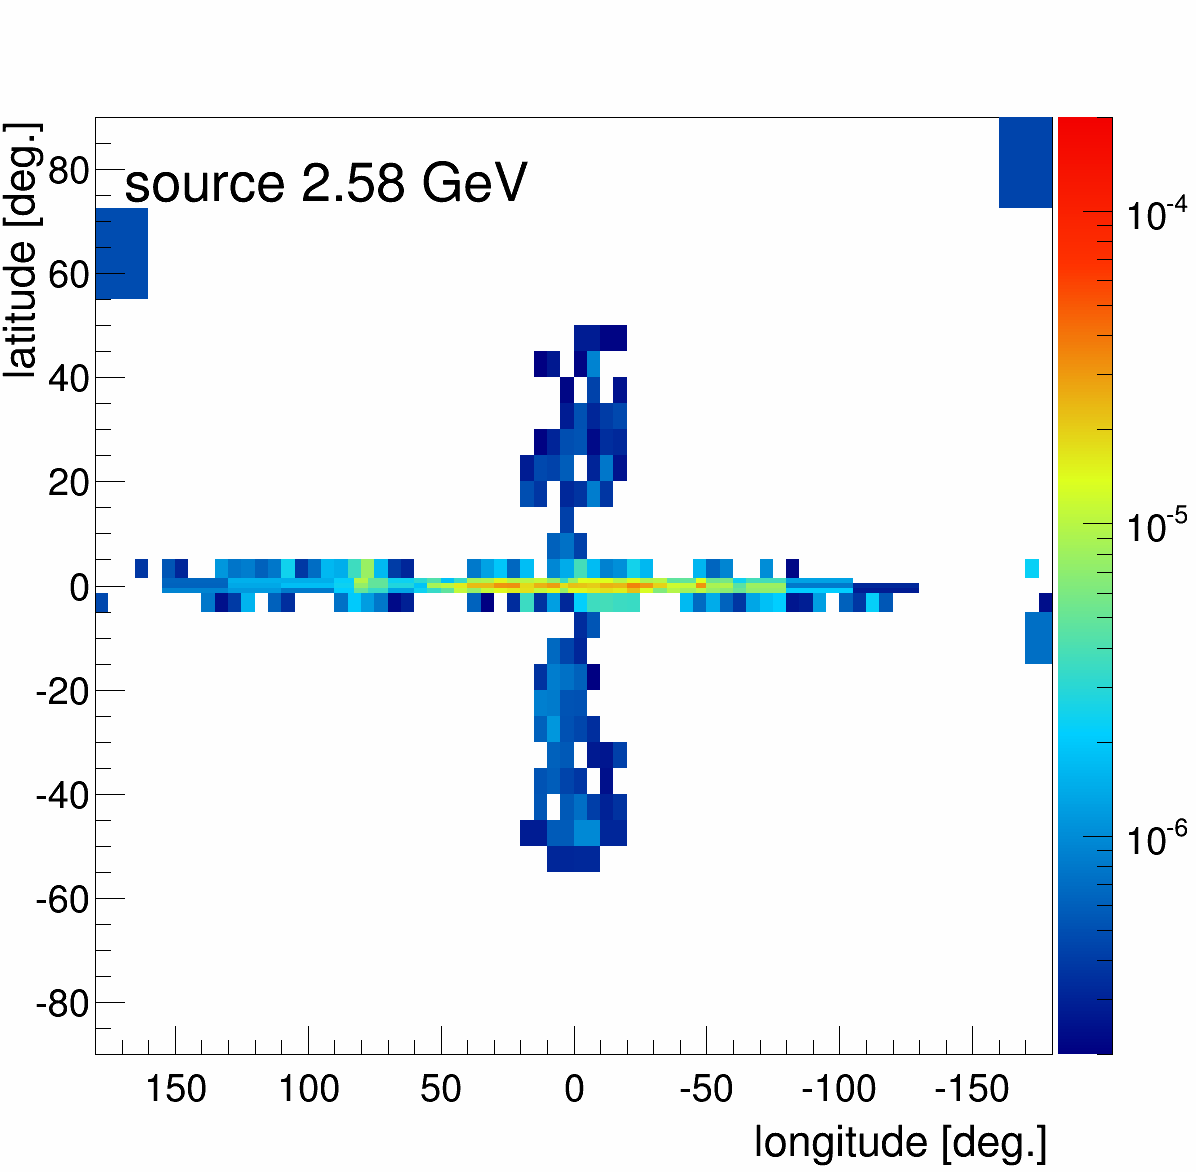
\includegraphics[width=1.\linewidth]{pic/results/MCRonly_SCR_fluxE12_skymap.png}
  	\subcaption{Flux distribution of SCR}
  	\label{fig:MCRonly_skymap_SCR}
  \end{minipage}
  \hfill
  \begin{minipage}[h]{0.45\textwidth}
  	\centering
	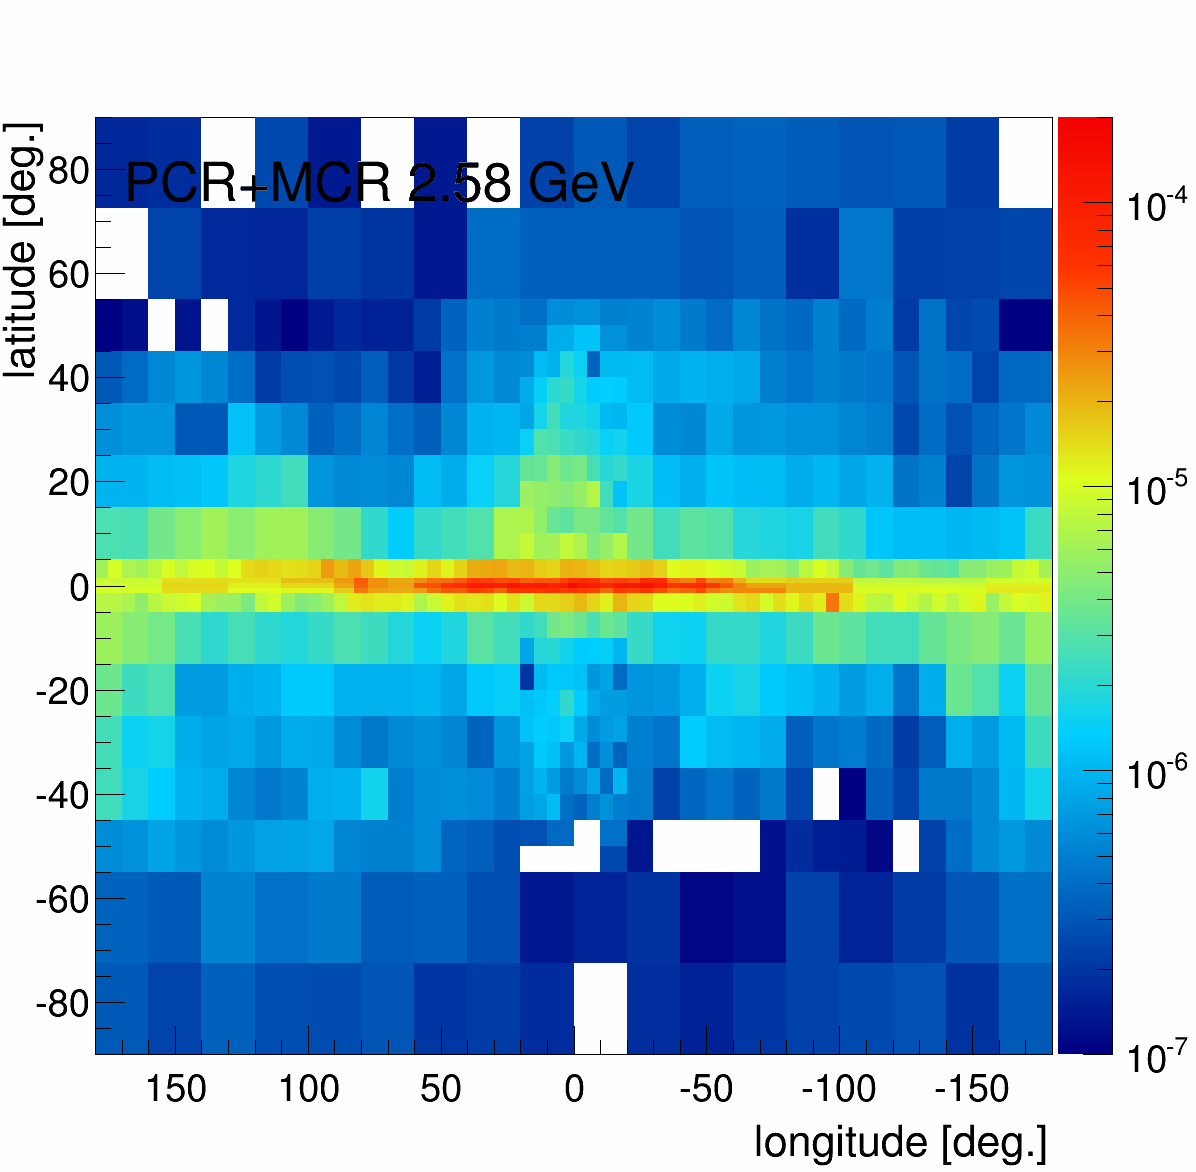
\includegraphics[width=1.\linewidth]{pic/results/MCRonly_PCR+MCR_fluxE12_skymap.png}
  	\subcaption{Flux distribution of PCR + MCR}
  	\label{fig:MCRonly_skymap_PCR+MCR}
  \end{minipage}
  \label{fig:MCRonly_skymaps}
\end{figure}

\subsection{Discussion on spatial shapes}

Fig. \ref{fig:MCRonly_skymaps} shows the spatial distribution of the flux of each component around 2 GeV, as returned by the fit.

The bremsstrahlung component is consistent with the the expectations. Present everywhere, it is strong in the disk, and decrease a little in the bubbles.

\todo{Though the general shape is spherical, the IC component has an unexpected feature in the form of a strong depletion in the disk, like a "sandwich" structure. This is surprising in the sense that this is where the interstellar radiation field (ISRF) and electron density are supposed to be maximal, creating a higher IC flux. A possible explanation could be coming from the dust distribution, screening the starlight component of the ISRF. Thus depriving the ISRF of its main component and leaving only the dust infra red emission and the CMB to interact with the electrons. This could result in a lower IC gamma-ray flux in the disk.}

The SCR component is playing his role, filling the bubbles and the disk, where the high energy portion of the spectra needs a harder spectrum. It traces the sources distribution in the disk and the outflow of high energy protons in the bubbles.

The general shape of PCR looks coherent with he shape of the galaxy, with a strong flux in the bar and the galactic disk in general. When looking closely, one can see the same kind of depletion in the disk than for IC, even if the effect is less remarkable. This finds its cause in the MCR distribution with a very high flux in the disk. The sum of both templates (MCR + PCR) shows no sign of such a feature, which tends to show that some of the PCR photons are absorbed by the MCR template. But the total is coherent, with no unexplainable central gap.

The MCR template also follows the spatial distribution of molecular clouds in our galaxy. It is a good sign since it is supposed to come from those regions.
It is not spherical at all. That could have happened if the excess component has a DM origin, since it is supposed to be spherically distributed.

\newpage

\section{Introducing SCR and DM}
%	-Introduction of SCR + DM
%		-chi2
%		-spatial shapes	
%		-Weniger plots
%		-Specklings

\begin{figure}[h]
  \centering
  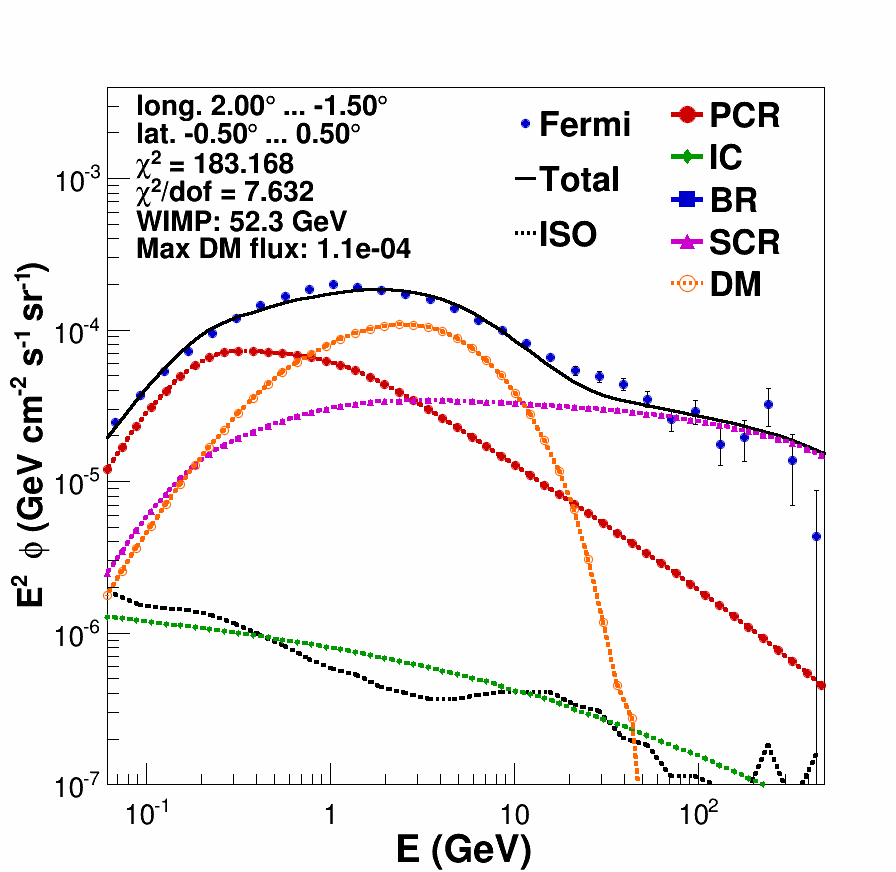
\includegraphics[width=.5\linewidth]{pic/results/DMonly_CMZ.png}
  \caption{spectrum of best mass DM fitted in CMZ. Also pictures of DM distribution compared to gas map.}
  \label{fig:DMonly_CMZ}
\end{figure}

\begin{figure}[h]
  \centering
  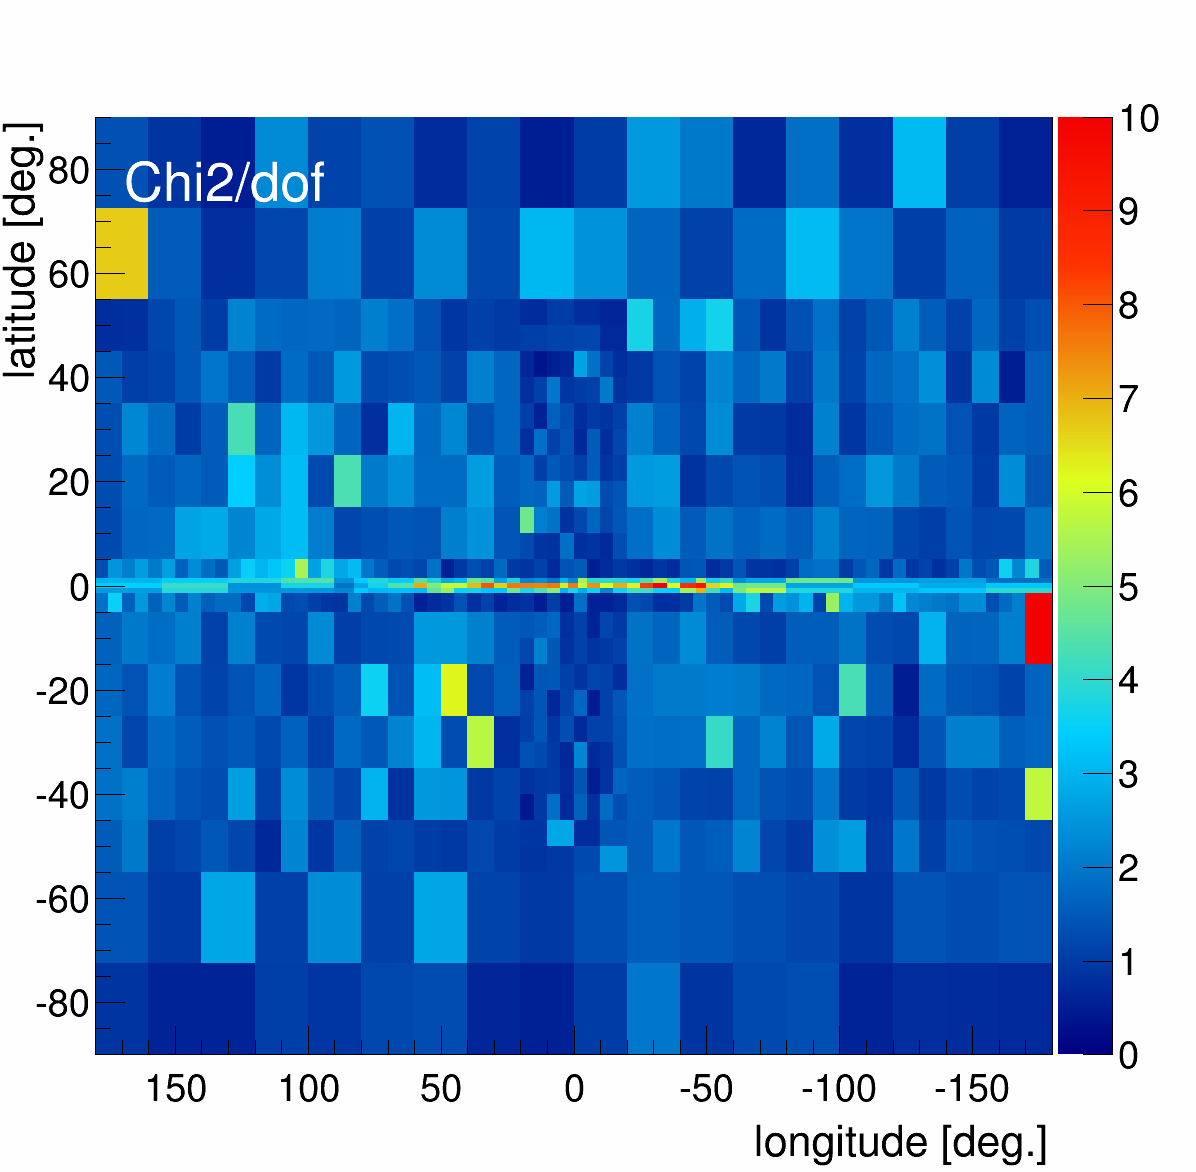
\includegraphics[width=.5\linewidth]{pic/results/DMonly_chi2Distribution.png}
  \caption{DM fit chi2 distribution}
  \label{fig:DMonly_chi2Distribution}
\end{figure}

\begin{figure}[h]
  \centering
  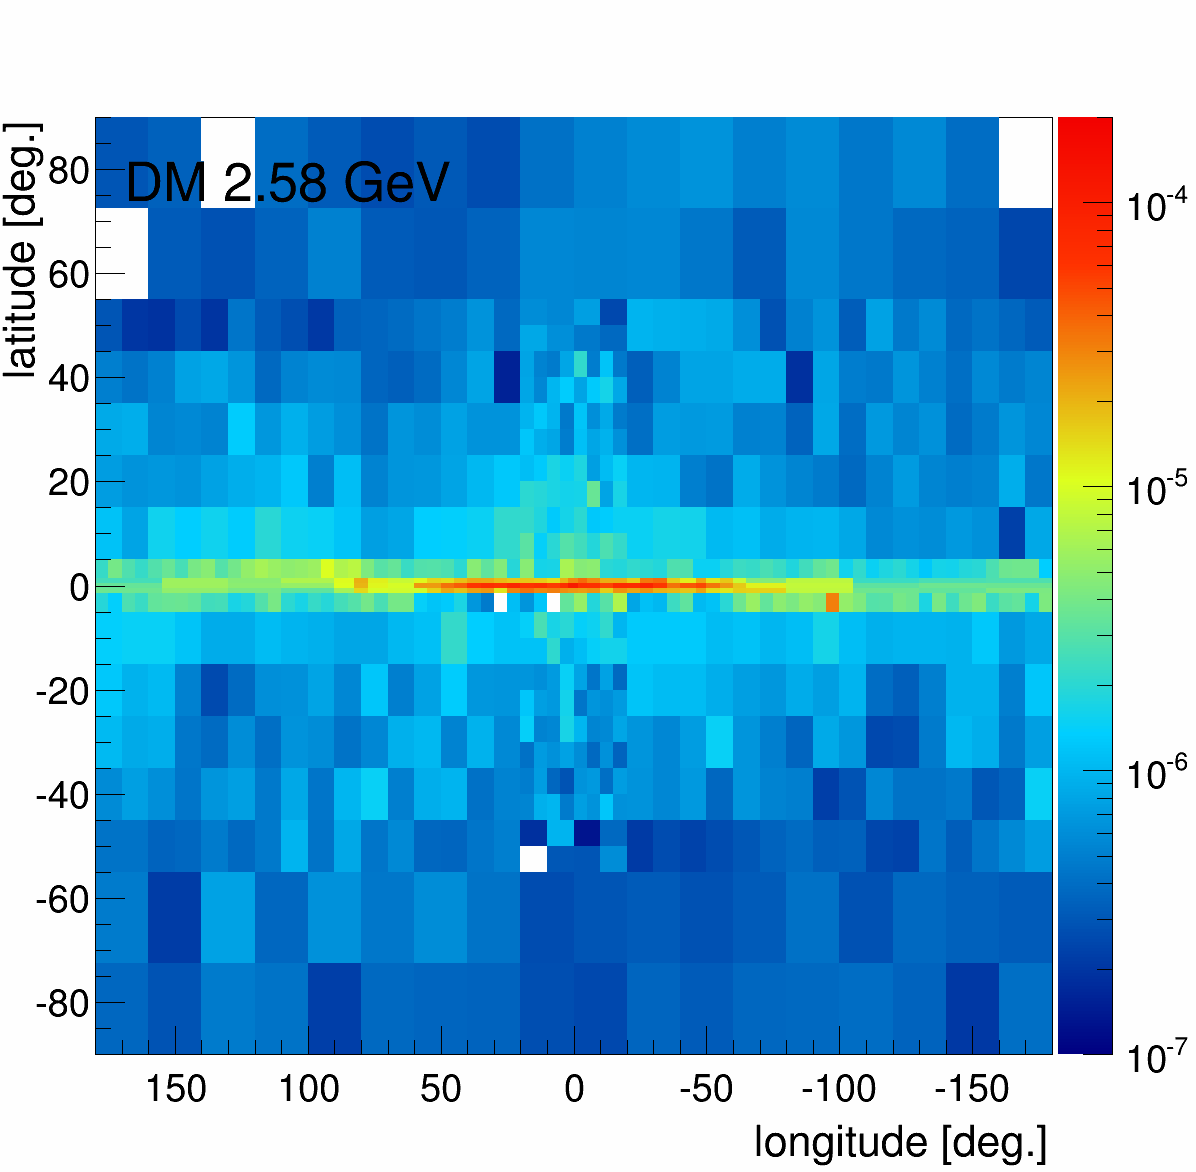
\includegraphics[width=.5\linewidth]{pic/results/DMonly_DM_fluxE12_skymap.png}
  \caption{DM distribution compared to gas map.}
  \label{fig:DMonly_skymap_DM}
\end{figure}


The first step is to determine which mass for the WIMP particles would produce the best spectrum for our fit. Fig. \ref{fig:DMonly_CMZ} shows the best fit for the CMZ region, with the WIMP mass as a free parameter. It chooses a mass of 52.3 GeV, peaking around a few GeV, as expected in \todo{ref theory section}. Since the excess is the most significant in this region, it is also the best place to define our mass for the rest of the sky. This is what is done in the following section.


Once the mass is determined for the entire sky, the fit gives the following results. The $\chi^2$ distribution (Fig. \ref{fig:DMonly_chi2Distribution} is comparable to the MCR fit for the major part but is significantly worst in the disk.


As seen on Fig. \ref{fig:DMonly_skymap_DM}, the DM distribution of the fit traces closely the distribution of molecular gas distribution (as traced by CO).

\newpage


\section{Introducing SCR and MSP}
%	-Introduction of SCR + MSP:
%		-chi2
%		-spatial shapes
%		-Weniger plots
%		-Specklings

\begin{figure}[h]
  \centering
  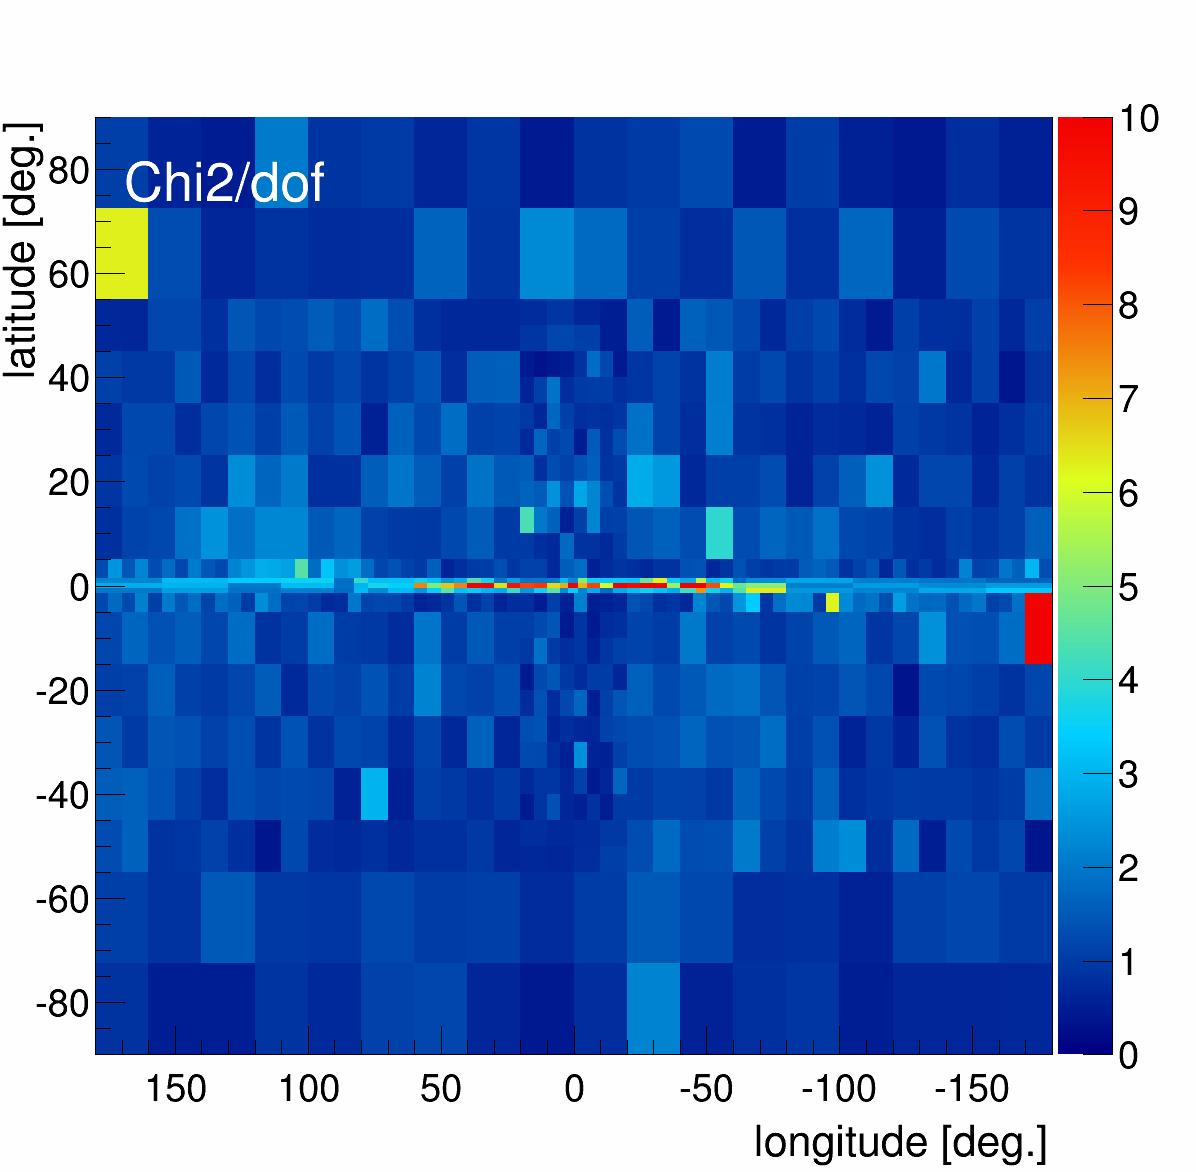
\includegraphics[width=.5\linewidth]{pic/results/MSPonly_chi2Distribution.png}
  \caption{Chi2 distribution of MSP only fit}
  \label{fig:MSPonly_chi2Distribution}
\end{figure}

The first thing that can be noticed when seeing the $\chi^2$ distribution of the MSP only fit (Fig \ref{fig:MSPonly_chi2Distribution}) is the similitudes with the DM only fit (Fig. \ref{fig:DMonly_chi2Distribution}). The fit succeeds pretty well outside the disk, but gets significantly worst when $|b| < 2°$.

\begin{figure}[h]
  \centering
  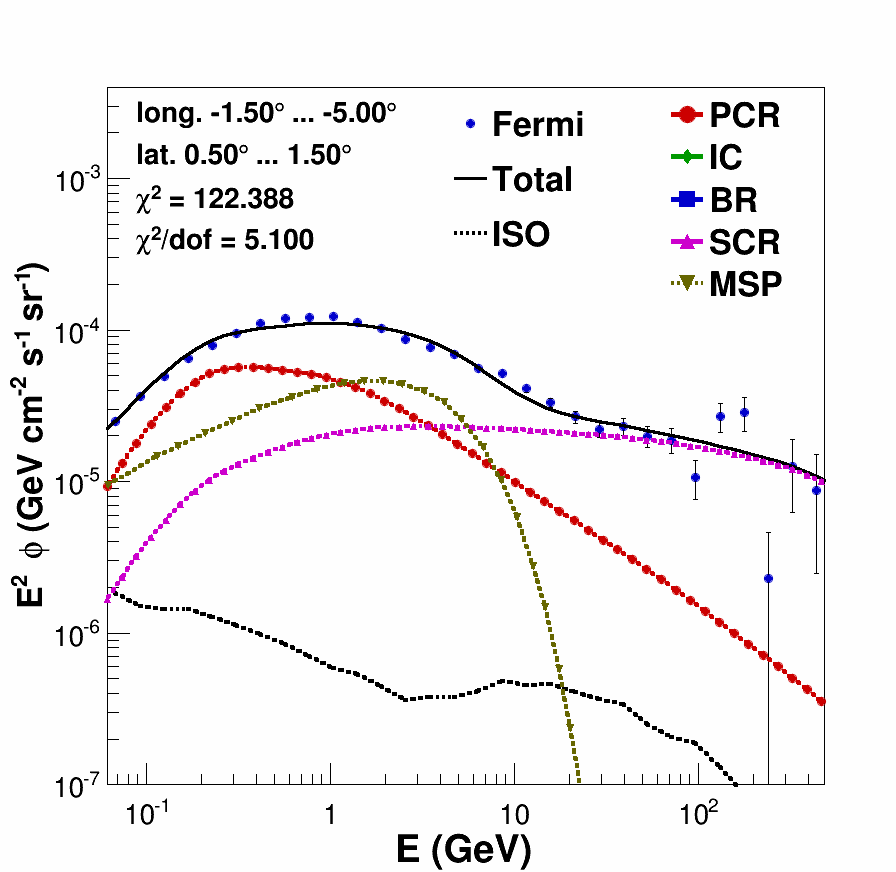
\includegraphics[width=.5\linewidth]{pic/results/MSPonly_CMZ.png}
  \caption{Fit with SCR and MSP spectrum in the CMZ region.}
  \label{fig:MSP_only_CMZ}
\end{figure}


Using the MSP spectrum predicted by fermi \todo{cite}  to fit the CMZ region does not give entire satisfaction. The CMZ is in the disk, where the $\chi^2$ is generally worst.



\begin{figure}[h]
  \centering
  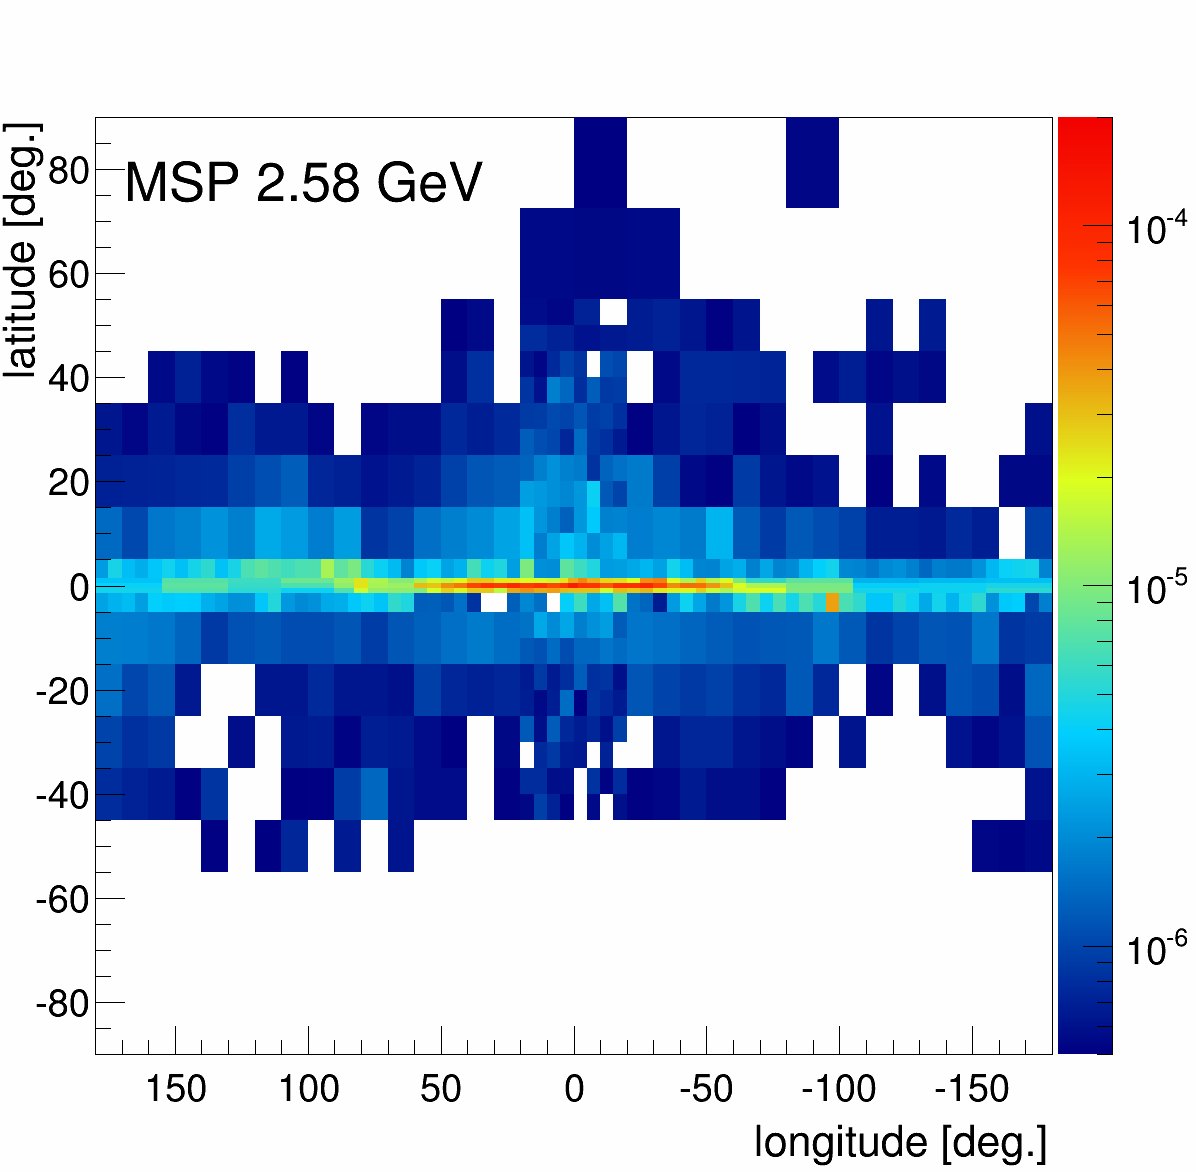
\includegraphics[width=.5\linewidth]{pic/results/MSPonly_MSP_fluxE12_skymap.png}
  \caption{Flux distribution of MSP around 2.5GeV.}
  \label{fig:MSP_only_CMZ}
\end{figure}

The distribution of MSP in the sky resembles the distribution of MCR and DM obtained in previous sections. Present everywhere in the disk, with a higher flux in GC and the bubbles.



\todo{add picture of residuals at low energy maybe?}

%Bad chi2 compared to MCR. The low energy spectrum is too hard.


















%% ==================
\chapter{To go further: How to improve the model}
\label{ch:discussion}
%% ==================
%This chapter is dedicated to a discussion of the results obtained in the previous Chapter \ref{ch:results}.
%Discussions what do they mean?:


%%%FOLLOWING SECTION IS DONE IN RESULT CHAPTER AS WE PRESENT THE MCR, DM AND MSP RESULTS
%\section{Comparison of all 3 excess templates}
%	-Comparison of all 3 templates -> best is MCR from the chi2 maps
%		-Comparison MCR vs DM
%		-Comparison MCR vs MSP
%		-Weniger plots
%		-Specklings
%	

%\section{Interpretation of spatial shapes}
%	-Interpretation of spatial shapes
%		-Expected features
%			-PCR			
%			-IC spherical
%			-BR a little everywhere, less in bubbles			
%			-SCR in disk + bubbles
%		-Sandwich in IC and PCR
%			-MCR replaces PCR -> There is more MCs in disk. Blocks PCR
%			-IC in disk mostly due to Dust and starlight is blocked by it. Dust is only a small portion compared to starlight -> decrease
%		
%		-Shape of the excess component		
%			-Shape of MCR, DM, MSP -> traces the CO map
%			-Only make sense with MCR
%			-DM and MSP have no reason to do that


\section{Discussion on the spatial distributions of the other components.}

The spatial distribution of a component can teach a lot about the fit. Every component is closely linked to a known physical process taking place in the Milky way. So even if the components contributions to a single cone can not be predicted, large scale structures  should emerge and coincide with the predictions. Using this, it is possible to verify the proper functioning of the fit by comparing the fitted spatial distribution of the different templates and the predicted one.
For example, the distribution of the ISRF is expected to be spherical around the GC in the UV range, where most of the starlight is emitted. It can also follow the dust distribution in the disk in the infra-red range. This can be used to check if the IC component is coherent in the fit and follows, to some extent, the ISRF distribution. Hopefully, the results show a spherical IC component centred on the GC.
The different distributions of each component will be discussed in the following section.

\subsection{PCR flux distribution}
The PCR component is produced by diffuse CR protons which collide with other hadrons and form a neutral pion, which in turn decays into two photons. So the PCR flux is directly proportional to diffuse CR, gas and dust density in the galaxy along the line of sight. It is expected to be present in every direction, with a stronger flux coming from the disc, and less from high latitudes.
The bubbles have a harder CR proton spectrum, but composed of source protons. This could imply that more high energy pion are created in those regions, and so the PCR flux should be more important. But this is not true since the presence of the SCR component. The latter was created specifically for such regions with a hard CR spectrum and should take care of that instead of PCR. This way, PCR should not mark too much the bubbles shape.

The results are very similar for the three fits, with MCR, DM or MSP. The galactic disk is clearly visible at all longitudes, up to twenty degrees in latitude. Some structures from the gamma ray sky are also here, with the bulge around the GC and diffuse shapes at the anti-center.
Looking carefully at the disk below two degrees in latitude near the GC, the flux decreases a little, when it is supposed to be the highest. Indeed, the GC is were the density of matter along the line of sight is the most important, and so PCR should follow it. This structure could be interpreted as the result of a higher concentration of molecular clouds in this area, cutting off low energy CR, as modelled by MCR. This effect could affect the proportion of PCR gamma-rays in favour of MCR and reverse the relative contributions. Thus MCR should replace PCR, but the sum of both component should still show an increase in flux toward the GC. Indeed, the sum skymaps is coherent (see appendix \ref{app:PCR+MCR_integral_distribution}). Like for the bubbles, the propagated proton CR spectrum changes too much to be described by a single power law. If this interpretation is correct and it is not just a fitting mistake, it is an other argument that can easily be explained by the MCR hypothesis, but not by DM or MSP.


\begin{figure}[h]
  \centering
  \begin{minipage}[h]{0.45\textwidth}
  	\centering
	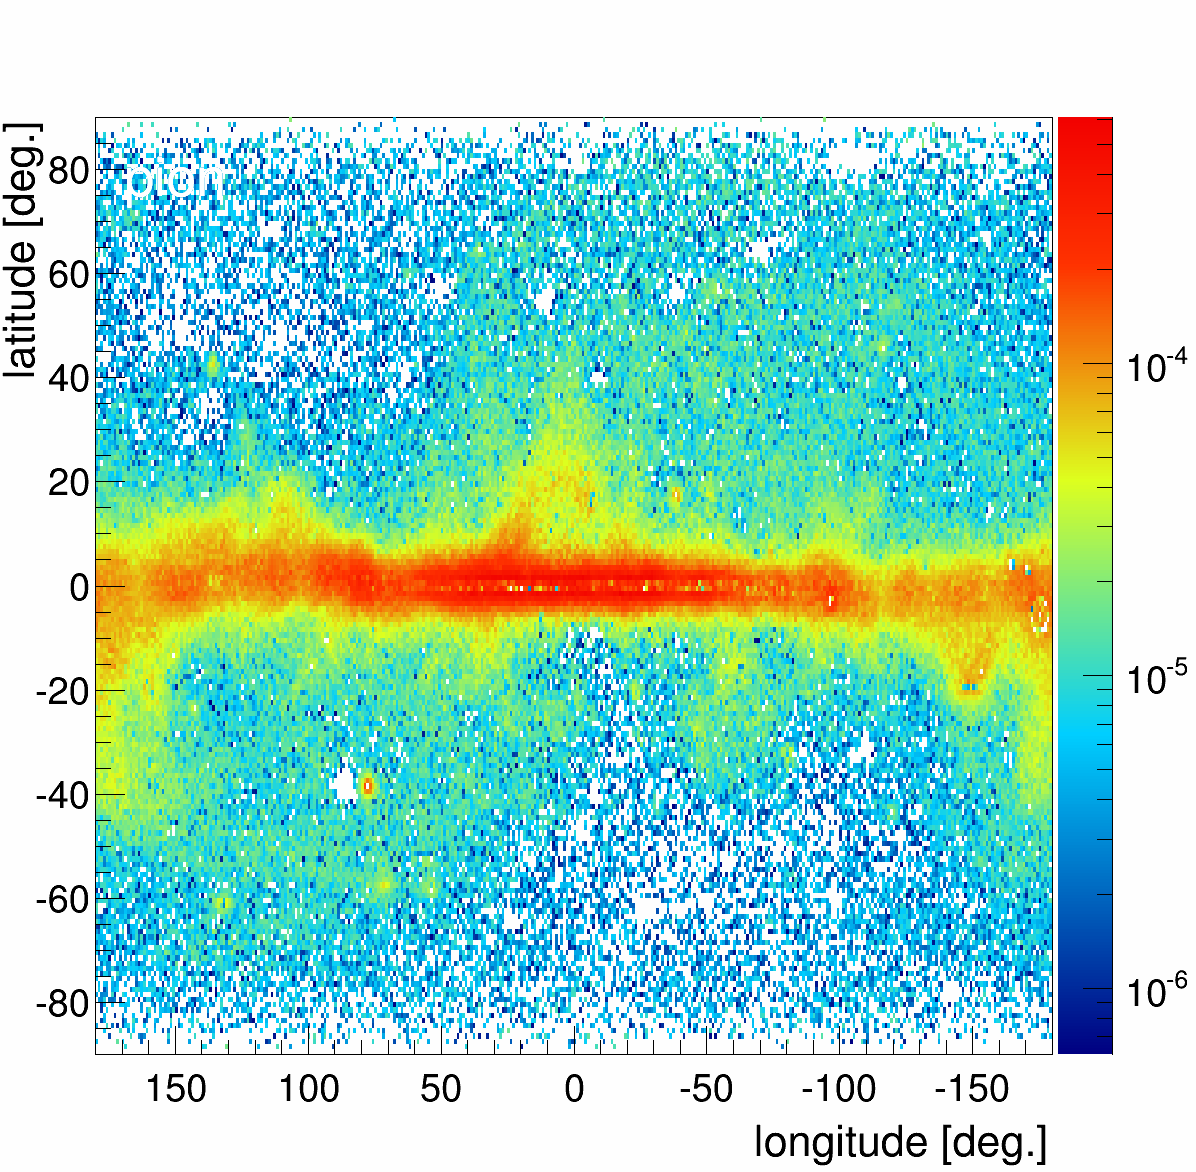
\includegraphics[width=1.\linewidth]{pic/discussion/MCRonly_fine_PCR_integral_distribution.png}
  	\subcaption{MCR}
  	\label{}
  \end{minipage}
  \hfill
  \begin{minipage}[h]{0.45\textwidth}
	  \centering
	  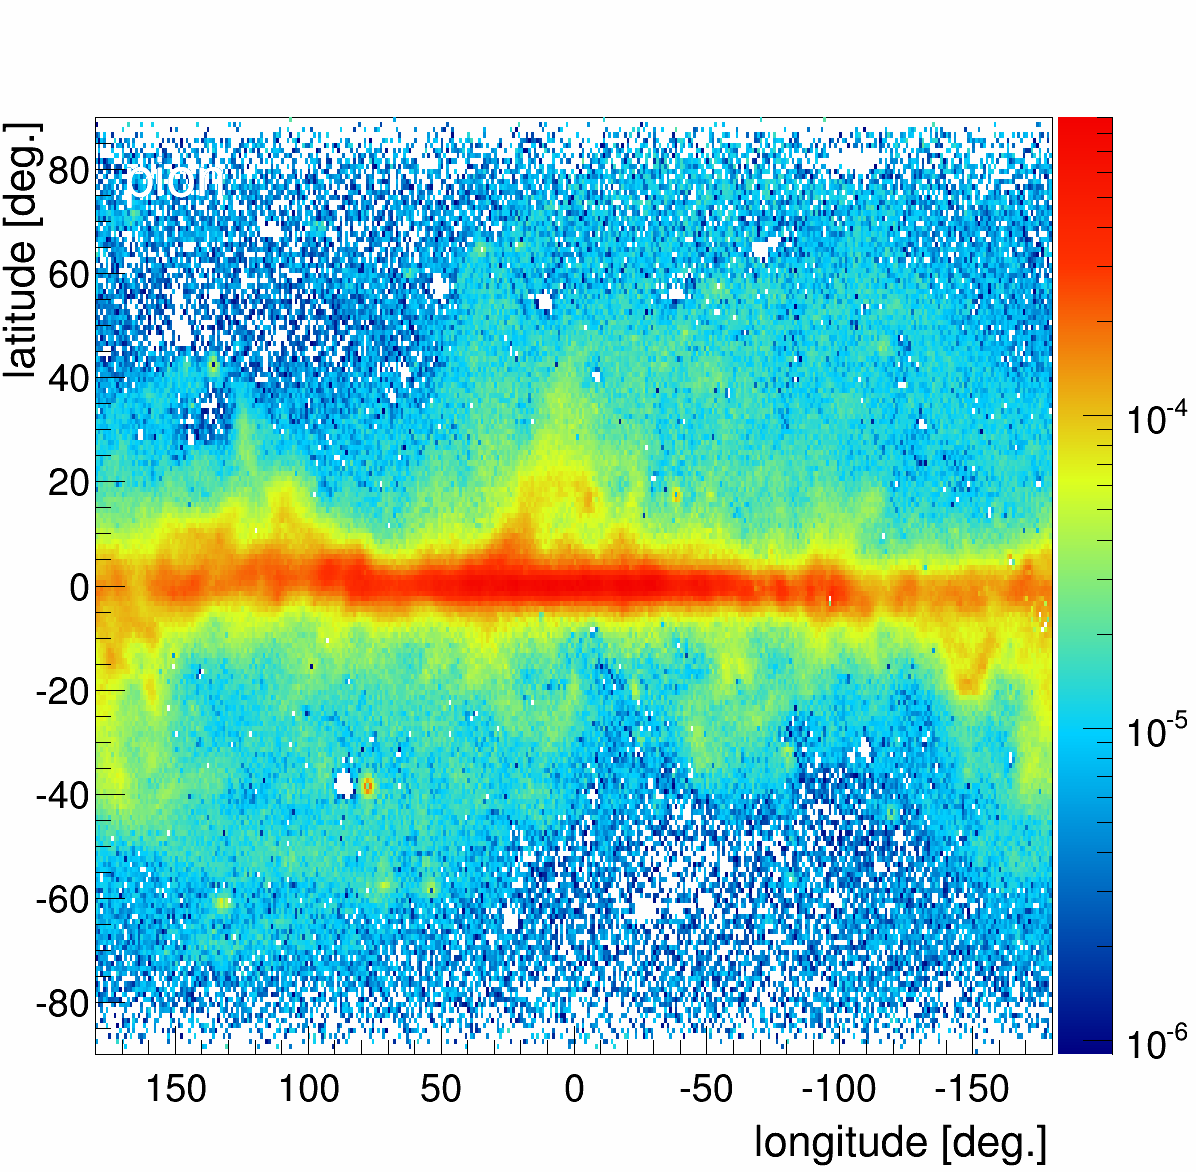
\includegraphics[width=1.\linewidth]{pic/discussion/DMonly_fine_PCR_integral_distribution.png}
	  \subcaption{DM}
	  \label{}
  \end{minipage}
  \hfill
  \begin{minipage}[h]{0.45\textwidth}
	  \centering
	  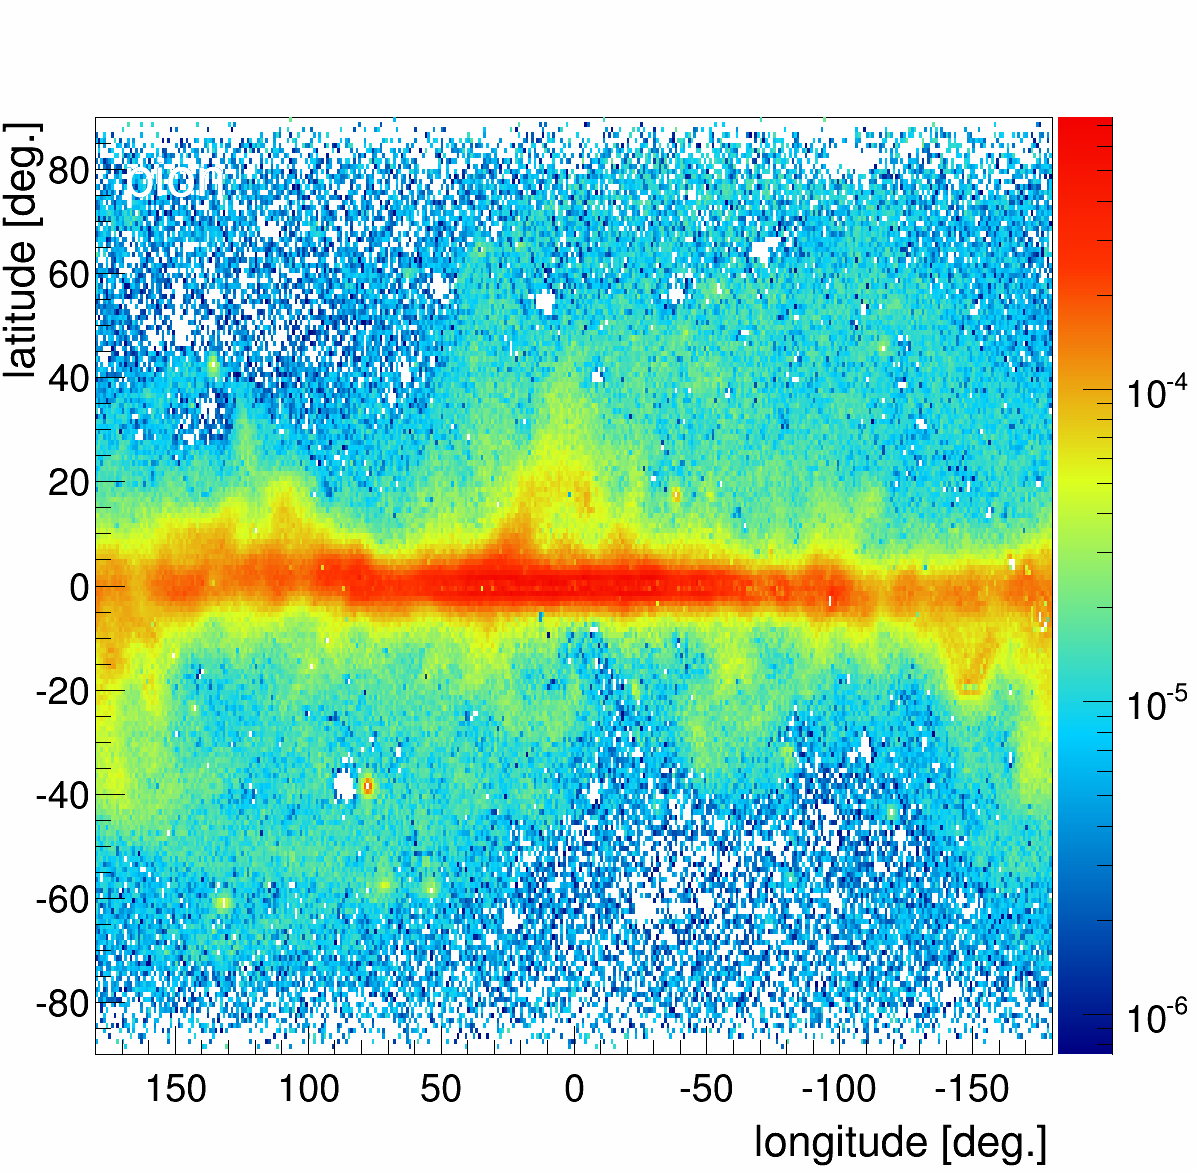
\includegraphics[width=1.\linewidth]{pic/discussion/MSPonly_fine_PCR_integral_distribution.png}
	  \subcaption{MSP}
	  \label{}
  \end{minipage}
  \caption[PCR spatial distributions.]{PCR spatial distribution with a MCR (a), a DM (b) and a MSP (c) fit. The galaxy disk and matter distribution is clearly visible. With MCR and to a lesser extend MSP, a drop in flux can be observed in the disk, below two degrees in latitude. This could be the excess component tracing MCs that take other PCR, tracing the propagated CRs.}
  \label{fig:PCR_flux_distrib_excess_comp}	 
\end{figure}


\newpage
\subsection{IC flux distribution}
The inverse compton scattering component is directly proportional to the ISRF and the electrons CR. Electrons are present everywhere in the galaxy, and the ISRF is dominant in the GC for the UV range, but follows the dust in the IR range and is isotropic in the radio. This distribution should be visible in the IC component of the fit.
Indeed, a spherical distribution can clearly be identified for the three different fits with DM, MCR and MSP. Nonetheless, there is a noticeable difference in the disk between the IC distribution for the MCR and DM fits and the MSP fit. In the MCR and DM fit, the disk presents a high IC flux when and MSP does not. On the contrary, the MSP fit presents a clear dip in the galactic disk. This gap is unexpected, since the ISRF is supposed to be the strongest in the disk, and the diffuse electrons are also produced mainly here. This effect could come from the shape of the MSP spectrum at low energies. Indeed, being softer than MCR and DM, and having a higher contribution in the disk where the excess is present, the fit overshoot the low energies under 1 GeV. This does not leave any space for an IC component that is also very soft. This is sown in figure \ref{fig:Excess_comp_comparison} where the only fit that does not need IC in the CMZ is the MSP fit.

\begin{figure}[h]
  \centering
  \begin{minipage}[h]{0.45\textwidth}
  	\centering
	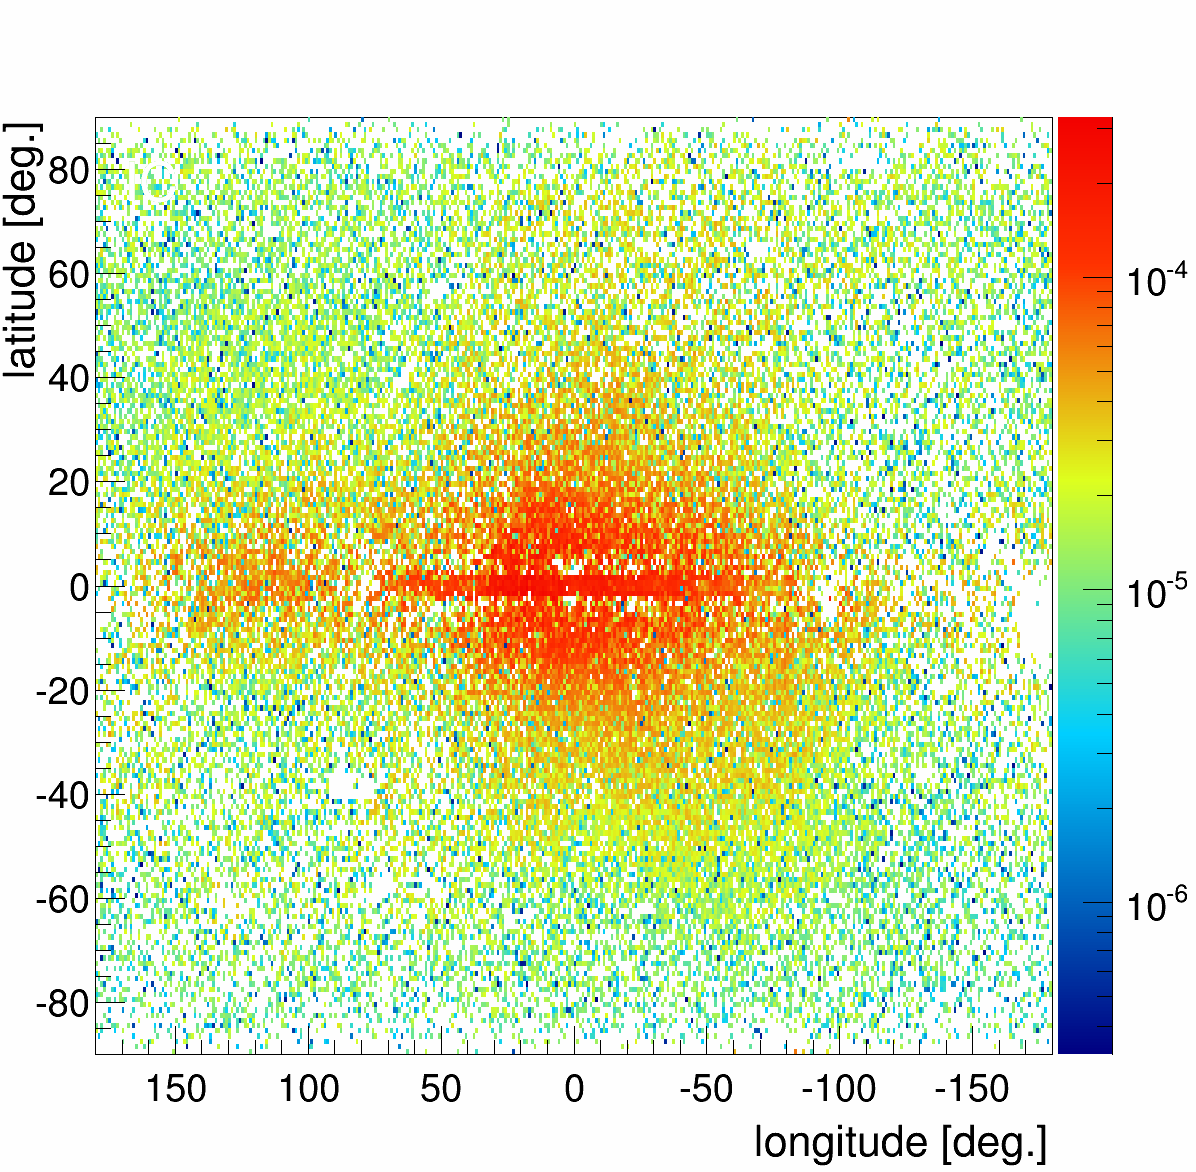
\includegraphics[width=1.\linewidth]{pic/discussion/MCRonly_fine_IC_integral_distribution.png}
  	\subcaption{MCR}
  	\label{}
  \end{minipage}
  \hfill
  \begin{minipage}[h]{0.45\textwidth}
	  \centering
	  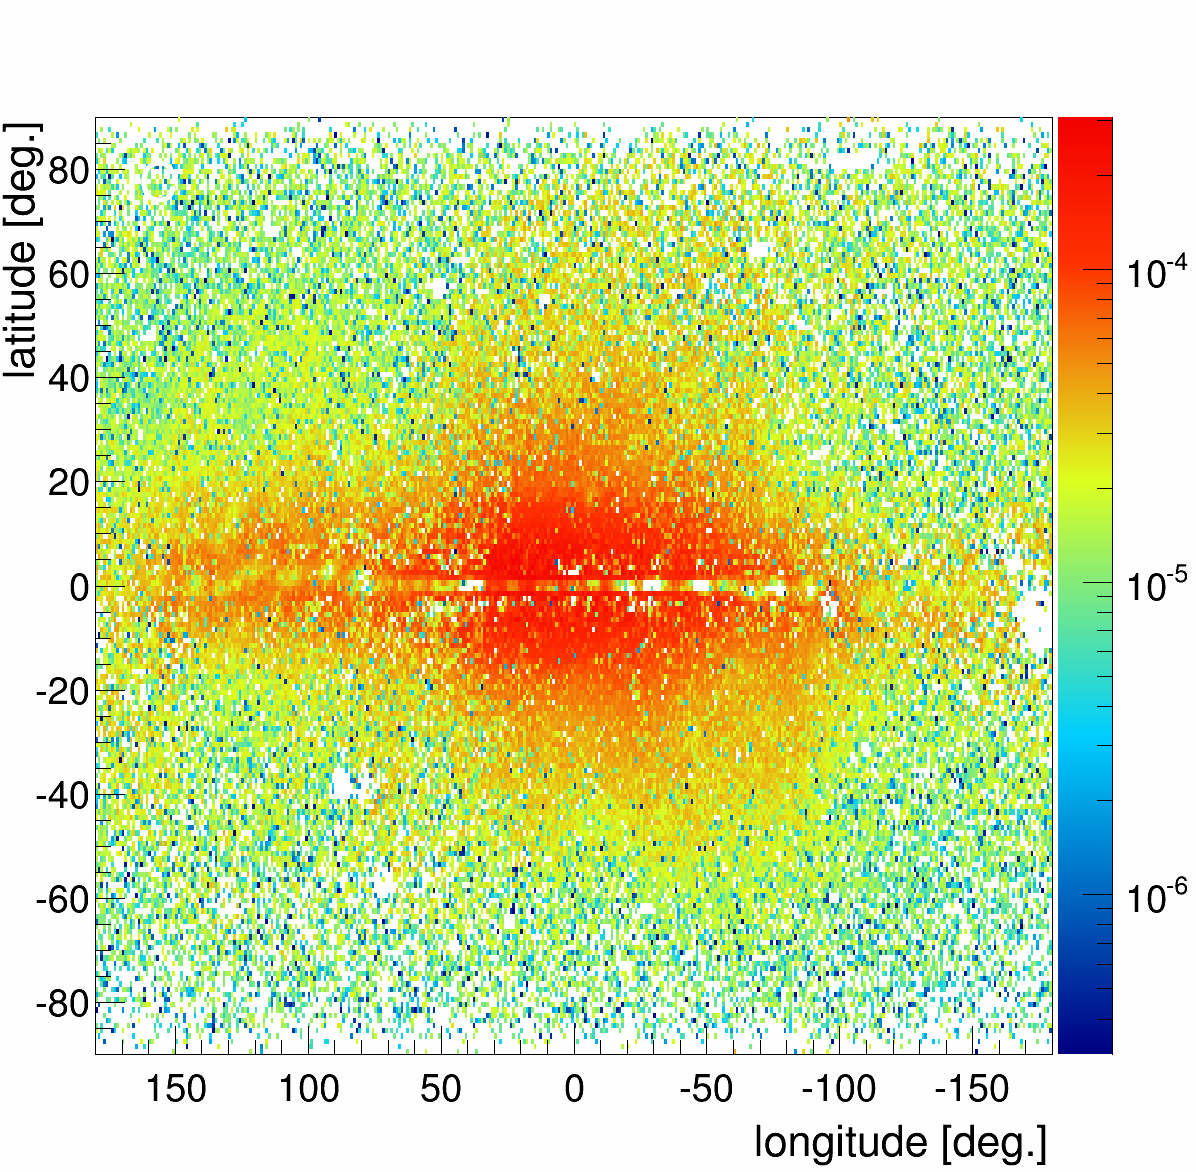
\includegraphics[width=1.\linewidth]{pic/discussion/DMonly_fine_IC_integral_distribution.png}
	  \subcaption{DM}
	  \label{}
  \end{minipage}
  \hfill
  \begin{minipage}[h]{0.45\textwidth}
	  \centering
	  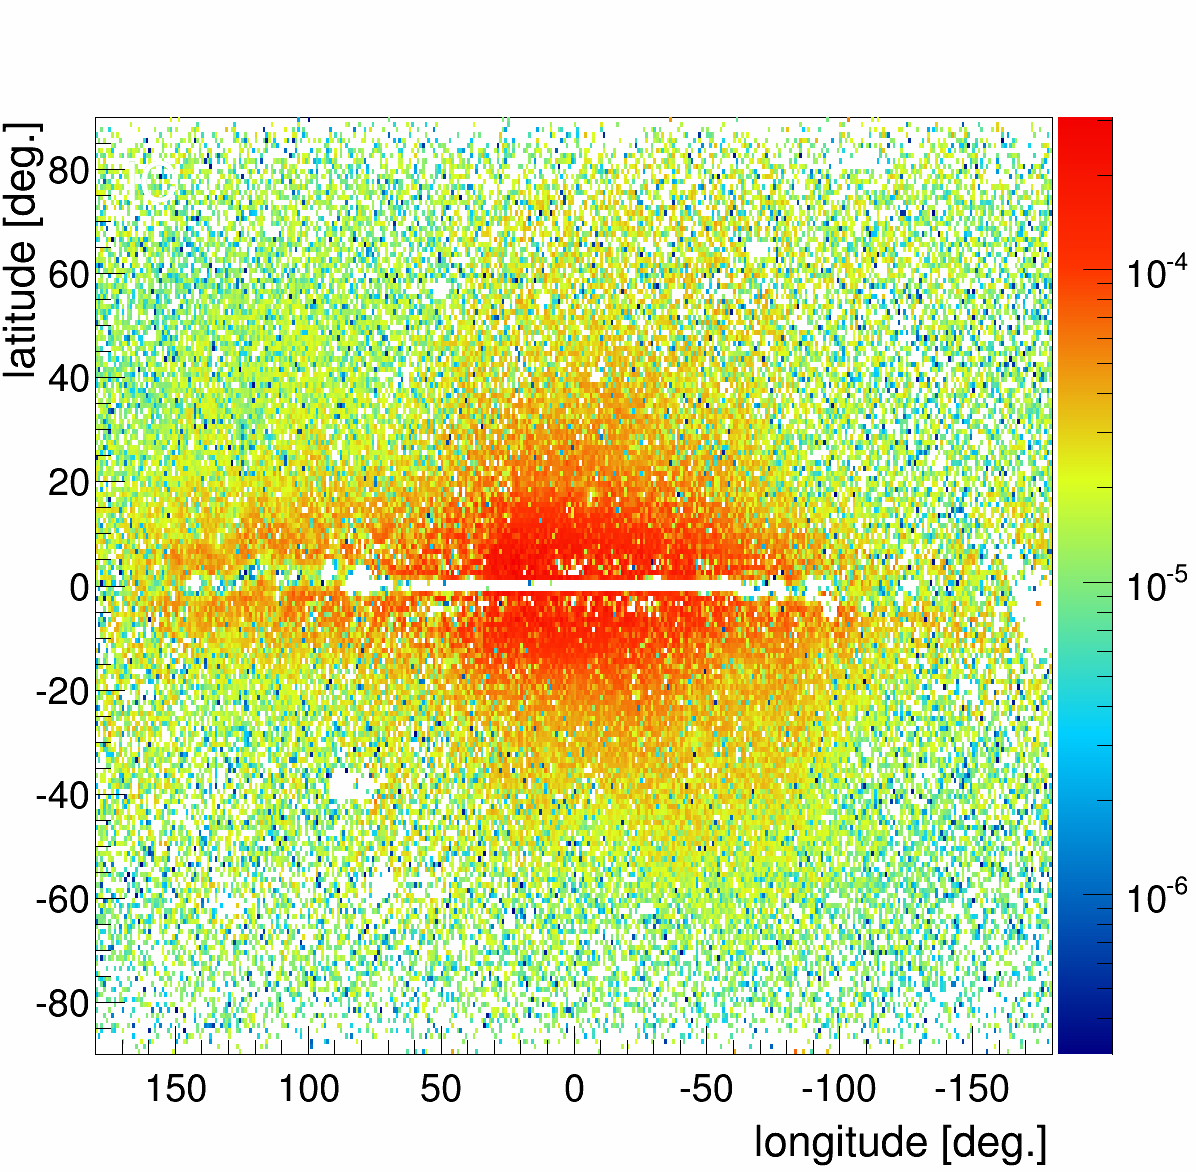
\includegraphics[width=1.\linewidth]{pic/discussion/MSPonly_fine_IC_integral_distribution.png}
	  \subcaption{MSP}
	  \label{}
  \end{minipage}
  \caption[IC spatial distributions.]{IC spatial distribution with a MCR (a), a DM (b) and a MSP (c) fit.}
  \label{fig:IC_flux_distrib_excess_comp}	 
\end{figure}

\newpage
\subsection{BR flux distribution}
The BR component is linked to the CR electron density along the line of sight and the electromagnetic fields in the galaxy. It should then be present everywhere. It is what can be observed in Fig. \ref{fig:BR_flux_distrib_excess_comp}, but some features are remarkable. Mainly the decrease of the flux in the disk and the bubbles.
Depending on the fit, the average flux is also changing. The BR component is a lot more present with the MCR fit than with DM, which in turn presents more BR than the MSP fit. The fact that the MSP fit does not use a lot of BR is consistent with the fact that the MSP spectrum is very soft at low energies. Since BR is also dominant at these energies, both can not have a high flux at the same time. The fit must do concession in order to use them both.

\begin{figure}[h]
  \centering
  \begin{minipage}[h]{0.45\textwidth}
  	\centering
	\includegraphics[width=1.\linewidth]{pic/discussion/MCRonly_fine_BR_integral_distribution.png}
  	\subcaption{MCR}
  	\label{}
  \end{minipage}
  \hfill
  \begin{minipage}[h]{0.45\textwidth}
	  \centering
	  \includegraphics[width=1.\linewidth]{pic/discussion/DMonly_fine_BR_integral_distribution.png}
	  \subcaption{DM}
	  \label{}
  \end{minipage}
  \hfill
  \begin{minipage}[h]{0.45\textwidth}
	  \centering
	  \includegraphics[width=1.\linewidth]{pic/discussion/MSPonly_fine_BR_integral_distribution.png}
	  \subcaption{MSP}
	  \label{}
  \end{minipage}
  \caption[BR spatial distributions.]{BR spatial distribution with a MCR (a), a DM (b) and a MSP (c) fit.}
  \label{fig:BR_flux_distrib_excess_comp}	 
\end{figure}
\newpage
\subsection{SCR flux distribution}
The SCR distribution is expected to follow the disc, where point sources can still remain, and the bubbles, where the proton CR spectra is harder. And indeed, the spatial distribution obtained in the three  different fits are similar and correspond perfectly to the expectations.


\begin{figure}[h]
  \centering
  \begin{minipage}[h]{0.45\textwidth}
  	\centering
	\includegraphics[width=1.\linewidth]{pic/discussion/MCRonly_fine_SCR_integral_distribution.png}
  	\subcaption{MCR}
  	\label{}
  \end{minipage}
  \hfill
  \begin{minipage}[h]{0.45\textwidth}
	  \centering
	  \includegraphics[width=1.\linewidth]{pic/discussion/DMonly_fine_SCR_integral_distribution.png}
	  \subcaption{DM}
	  \label{}
  \end{minipage}
  \hfill
  \begin{minipage}[h]{0.45\textwidth}
	  \centering
	  \includegraphics[width=1.\linewidth]{pic/discussion/MSPonly_fine_SCR_integral_distribution.png}
	  \subcaption{MSP}
	  \label{}
  \end{minipage}
  \caption[SCR spatial distributions.]{SCR spatial distribution with a MCR (a), a DM (b) and a MSP (c) fit.}
  \label{fig:SCR_flux_distrib_excess_comp}	 
\end{figure}



\newpage
\section{Adding the MBR component}

\subsection{MBR fixed to MCR, magnetic cut-off}
\todo{add pictures of graph and skymaps}

The theory behind the MCR component involves a magnetic cut-off for low rigidity CR protons, that changes the gamma-ray spectrum at low energies. Such a cut-off only depends on the rigidity of the CR and the intensity of the electromagnetic field. So there is no reason for it to be only applied to protons, and not to electrons. This is the reasoning that led to the introduction of a new template, called MBR in the fit, equivalent to the BR template, but calculated from a different electron CR spectrum.
This new CR spectrum is composed of two different power laws for high and low energies, joigning at the break position. It has the exact same spectral indexes than the CR spectrum used for IC and BR, but the break is moved up, between 6 and 14 GeV, to stay consistent with the MCR break. The fit method is the same, and the MBR break is fixed to the MCR brake in a given region. This way, the magnetic cut-off is applied the same way to the electrons and protons CR. Once again, this component is expected to follow the MCs distribution.

A MIC component was tested as well, but it was not kept for physical reasons. First, the ISRF is not dependent of the electromagnetic field, photons do not carry any electric charge. It is also present in MC, where stars are formed and evolve.


\newpage
\section{Add DM late}

\todo{difference with DM+MCR. Results and discussion.}

Now the results are clear. MCR is a good solution to the gamma-ray GeV excess in the GC, and could replace the first hypothesis of the DM halo or hidden MSPs. Yet, the DM theory is strongly supported by other measurements \todo{cite}, for example the rotation curves of galaxies, and is one of the most important question of modern physics. And the fact that it is not the primary cause of the effect observed here does not mean it does not exist. On the contrary, under the hypothesis that MCR is really the cause of the excess, the fit could put strong limits on the DM models.

This section will present a few ways to study the current DM WIMP model using the fit method of this thesis.

\subsection{DM and MCR}

\todo{add figure}
A first idea is to let the fit choose for every cone the template that offers the best $\chi^2$ value. Taking a 52.3 GeV WIMP mass and the MCR template with free breaks, the fit has the choice between the two. The results are without much surprise in favor of MCR. Indeed, the previous comparisons of the $\chi^2$ distribution for a MCR or a DM fit showed a clear preference toward MCR. The $\chi^2$ map of a MCR fit is flat around one, even in the disk, whereas a DM fit does not work well for small latitudes. It is then only expected that the fit chooses MCR when it has the choice.

\subsection{DMlate}

This method can not say much else than what was already showed in the previous sections. The second idea that comes to mind is to take the MCR template for granted, and see if their is space to add DM contribution at the end of the fit. In other words, a first fit is performed with the classical templates (PCR, IC, BR), the source (SCR) and the MCR templates. Once the best relative contributions are found, the fit tries to add a DM template to improve the $\chi^2$.
Following the Ockham's razor principle, the least amount of contributions are accepted as true, and any additional component must be treated carefully. This way, the necessity of a DM template is checked, and it contribution can not be mistaken for a classical one.
\todo{add pic}
Such a fit was performed and the results will be discussed in this section. First of all, the DM flux distribution  is very sparse and degrees of magnitude below the other components. This was expected since the $\chi^2$ of the MCR only fit was already good. Only very small changes could improve it without changing the classical contributions. Using the same CMZ region in the GC, the optimal mass was determined to be \todo{mass DM late}.

Further studies of this kind could help to determine limits on the DM particle mass and cross-section.

\newpage
\section{How do these results fit in context}
%How do they fit in context:
%	-DM explanation
%		-Best mass around 50 GeV
%		-Increase goodness of fit
%		-Not spherical at all
%		-Follows CO map when there is no reason to do it
%	-MSP explanation
%		-Spectra too soft at low energies.
%		-Same problem than with DM.
%		
%	-What's new?







%% ==================
\chapter{Conclusion}
\label{ch:conclusion}
%% ==================

%
%Conclusion
%
%Resume what I did
%	-> fit
%	-> method
%
%Results
%	-> MCR is the fit winner
%	-> DM and MSP also work, but do not follow their predictions
%
%Opening
%	-> Put limit on DM mass and cross-section
%	-> Find other ways to study DM
%

Using a simple, well constrained, fitting method, the entire gamma-sky was modeled in a wide energy range. This allowed a spatial as well as a spectral study to be developed around the GC gamma-ray excess. High spatial resolution up to one by one degree bins were achieved, allowing a very detailed study of the excess distribution.

Three main hypothesis for the GC gamma-ray excess were tested and compared, namely the dark matter (DM), milli-second pulsars (MSP) and molecular clouds cut-offs (MCR). The results makes the MCR hypothesis stand out from DM and MSP. First, the spectral shape of the MCR component is more adapted to the excess spectral shape, making it easier for the fit to use. High energies as well as low energies can be fitted properly for any given region of the sky. On the contrary, MSP and DM have spectral features that do not allow a proper fit everywhere, especially the very soft spectrum above 10 GeV, making them insignificant for higher energies. Second, comes the general spatial distribution of the excess component in the fits. All three looks alike, following the disk and galaxy general shape, but only MCR is supposed to do so. Indeed, DM and MSP are expected to be distributed spherically around the GC, and they have no reasons to follow the galactic matter distribution. And finally, when looking at the details of the GC, and in particular the CO distribution, one can see a correlation between the excess component flux and the CO emission. This last result gives again a clear indication in favor of MCR, since it is the only component directly linked with molecular clouds. Overall, MCR was preferred by the fit and gives a explanation for the GC excess while staying in the standard model of physics.

Several path were followed to try and improve the model, taking MCR as the excess component. A new component (MBR) was introduce, following the same reasoning than MCR, but with the electron CR. Since their proportion is smaller, the effect of this new template is expected to be smaller.




%% --------------------
%% |   Bibliography   |
%% --------------------
\cleardoublepage
\phantomsection
\addcontentsline{toc}{chapter}{\bibname}

\bibliographystyle{achemso}
%\bibliographystyle{abbrv}
												  
% Use IEEEtran for numeric references
%\bibliographystyle{IEEEtranSA})

\bibliography{thesis}
%\nocite {*}	%Cite every citation in the bib file, even if they are not cited in the text

%% -----------------------
%% |   List Of Figures   |
%% -----------------------
%\cleardoublepage
%\phantomsection
\listoffigures

%% ----------------
%% |   Appendix   |
%% ----------------
\cleardoublepage
%% ==============================
%\chapter{Appendix}
%\label{ch:Appendix}
%% ==============================

\appendix
\addchap{Appendix}

\section{Some appendix section}
\label{app:fitresults}
This appendix chapter contains ...

%% ------------------------
%% |   Acknowledgements   |
%% ------------------------
\cleardoublepage

%\include{acknowledgements}

\end{document}
